\chapter{Results and Discussion}
In this section, the results of the path-following and position controller agents are used to compare the stochastic training and deterministic training agents. First, the results of both agents training in a small state environment are shown. Then, the results of increasing this state space are shown with each agent being tested outside their training data. Next, the stochastic agent was used to develop a position controllers for the quadcopter. Stabilizing and trajectory tracking results are shown. The controller was then tested against external disturbances. Finally, the controller was proven through simulation to be compatible with different quadcopters..

\section{Path-following Agent Training Results}
\subsection{Small State Space Training}
The objective of this training was for the agent to stabilize the quadcopter at a fixed point of [0,0,1] starting from a random position in each episode. Both the stochastic and deterministic training ran for a total of 3,600,500 steps. Fig. \ref{SvT0.5} shows the mean reward obtained by each agent. The stochastic training had a faster learning time with the model reaching its maximum reward of 264,370 at the time step of 2,629,500, while the deterministic training had a slower learning time with the model reaching its maximum reward of 244,510 at the time step of 3,582,440. Although the difference in the maximum reward is not large, the deterministic training took about 1,000,000 fewer steps to reach the maximum reward.
\begin{figure}[H]
\centerline{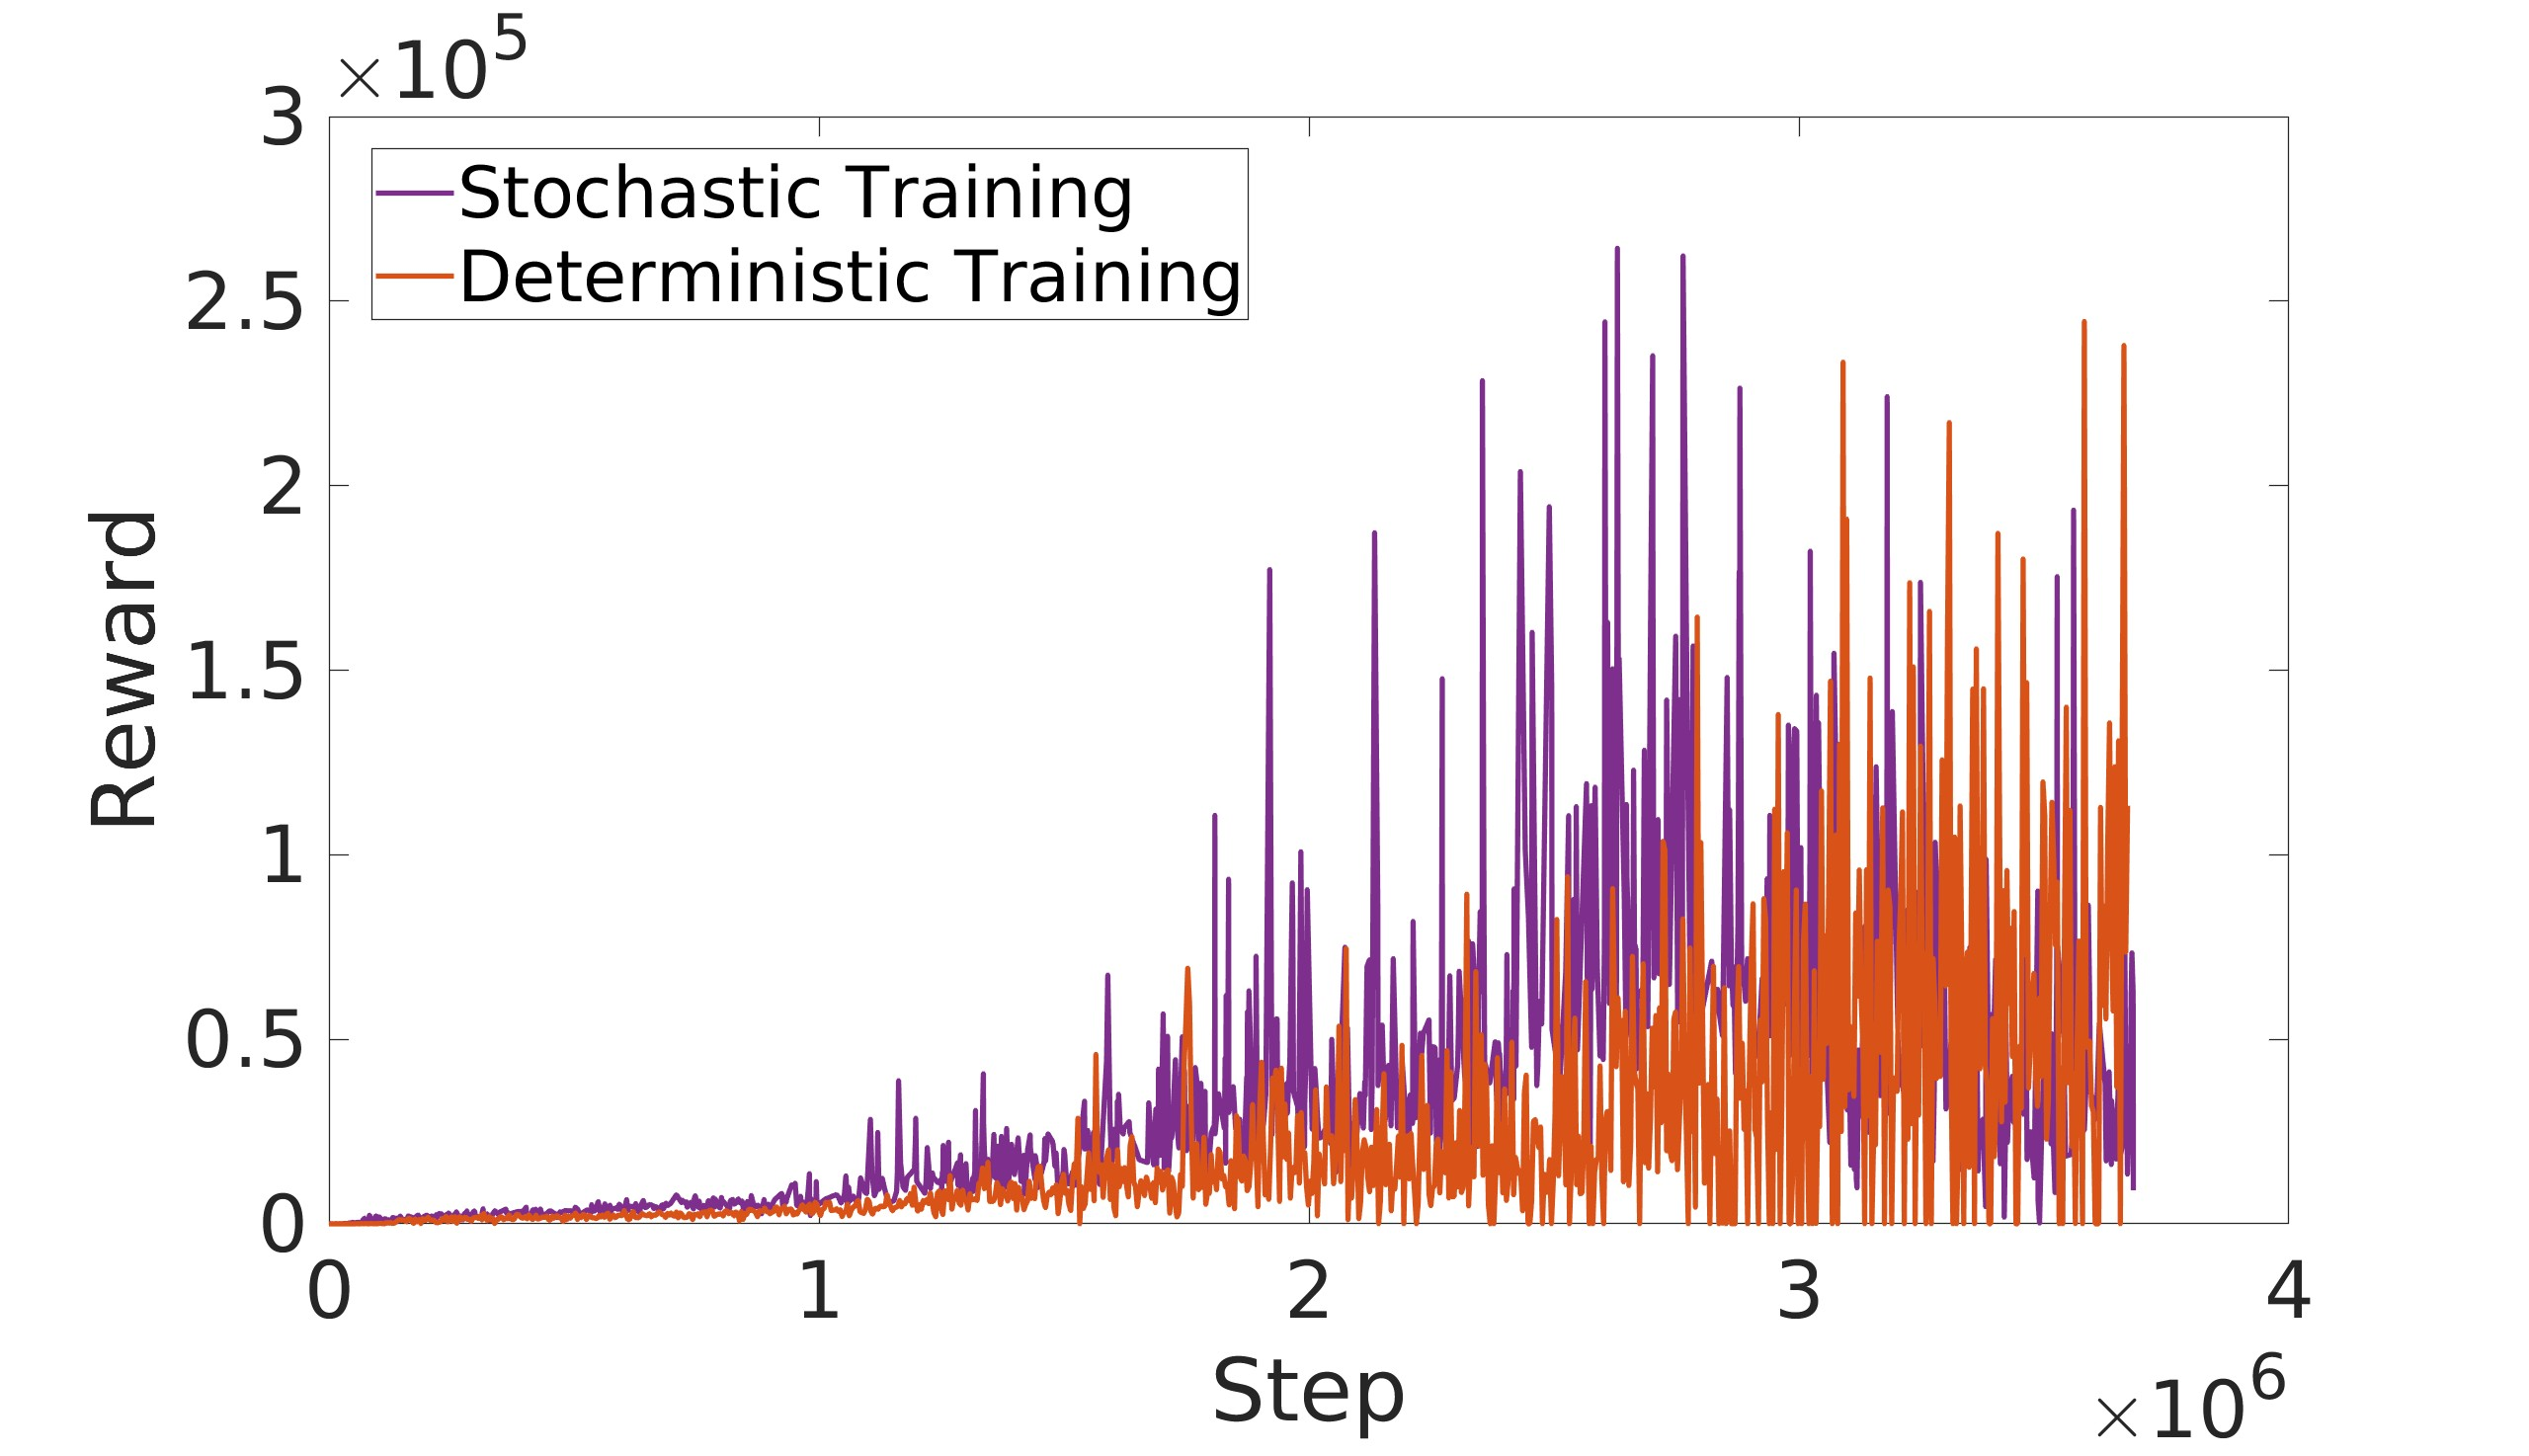
\includegraphics[width=0.8\textwidth]{plots/SACvsTD30_5.jpg}}
\caption{Average Mean Reward of Small State Space Training for Stochastic and Deterministic Training}
\label{SvT0.5}
\end{figure}
Fig. \ref{x0.5} shows the stochastic agent response when starting from an initial position of [-0.5, 0.5, 1.5] compared to the deterministic agent response. This point was chosen as the most extreme position the agents were trained on. Both agents stabilized with zero steady-state errors. As shown the performance of both agents is almost identical with negligible differences between the two algorithms.
\begin{figure}[H]
            \centerline{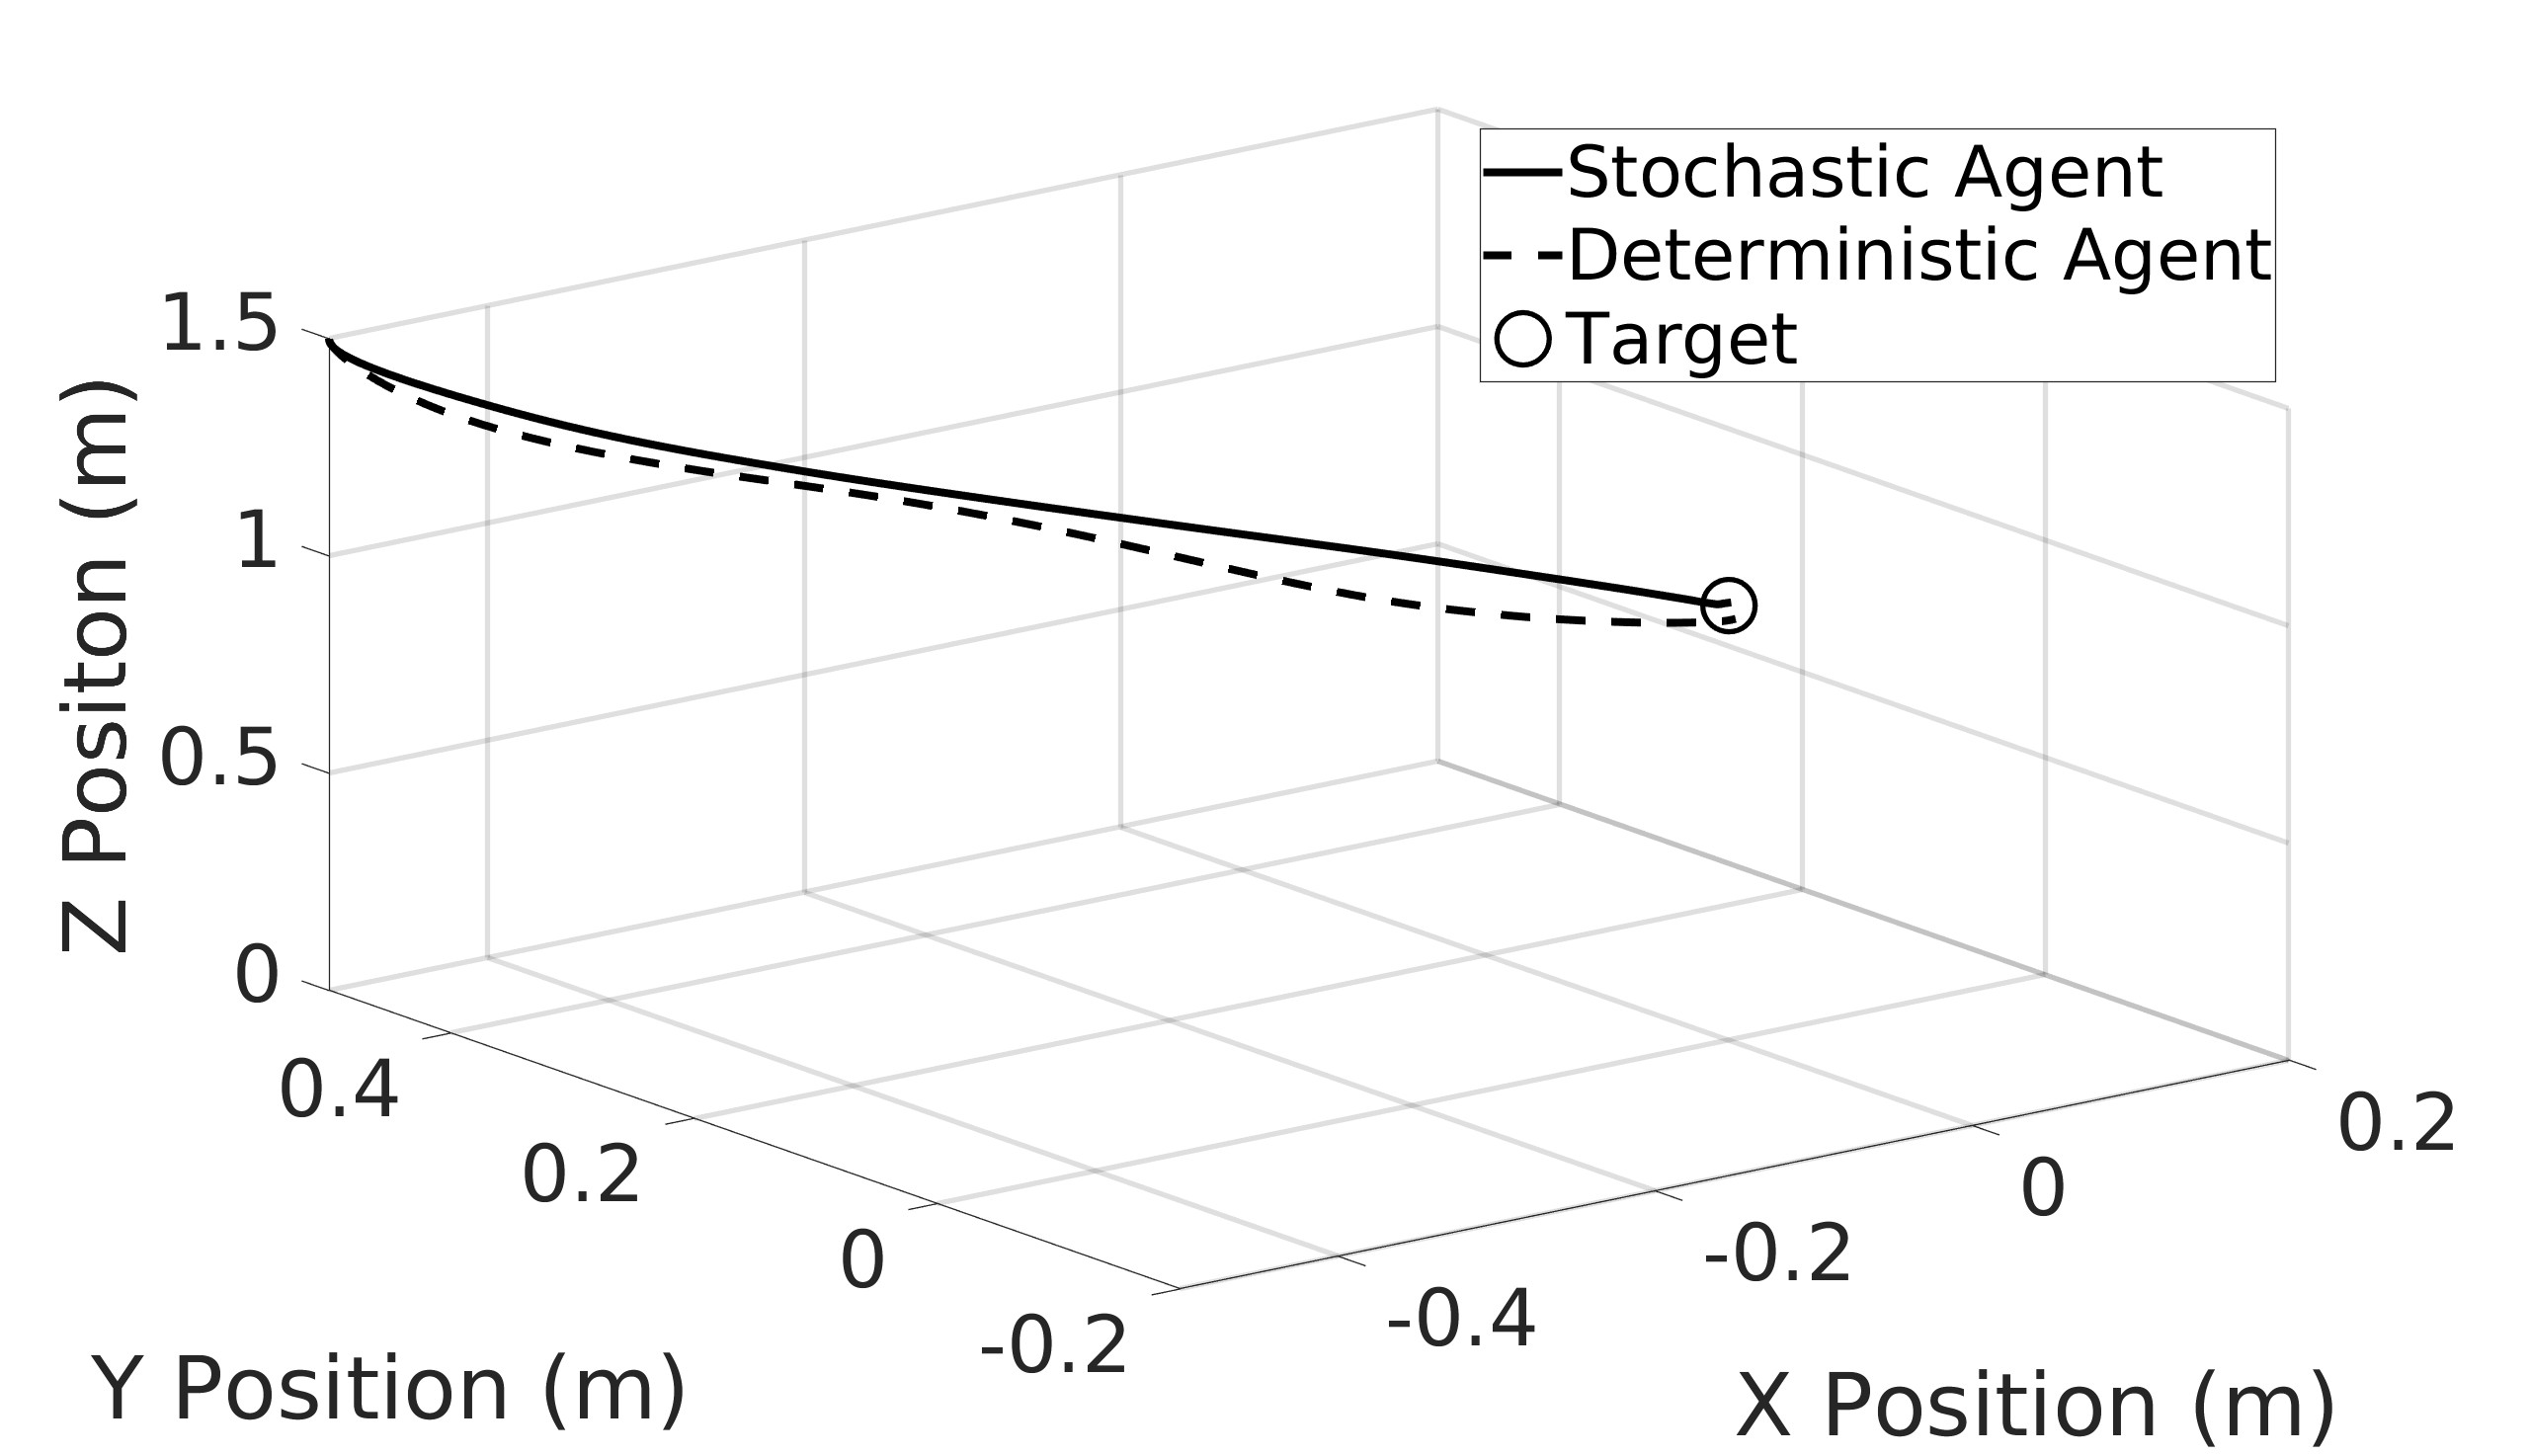
\includegraphics[width=0.735\textwidth]{plots/0_5_1.jpg}}
            \caption{Small State Space Response of an Initial Position of [-0.5, 0.5, 1.5] for Deterministic and Stochastic Agents}
            \label{x0.5}
    \end{figure}\clearpage
        The real difference between the two algorithms starts to appear when passing initial positions to the agent outside the trained state space. For the deterministic agent, it failed to stabilize and crashed almost immediately when starting with an initial position of [-0.8, 0.8, 1.4] as shown in Fig. \ref{offT0.5}. 
    \begin{figure}[H]
            \centering
            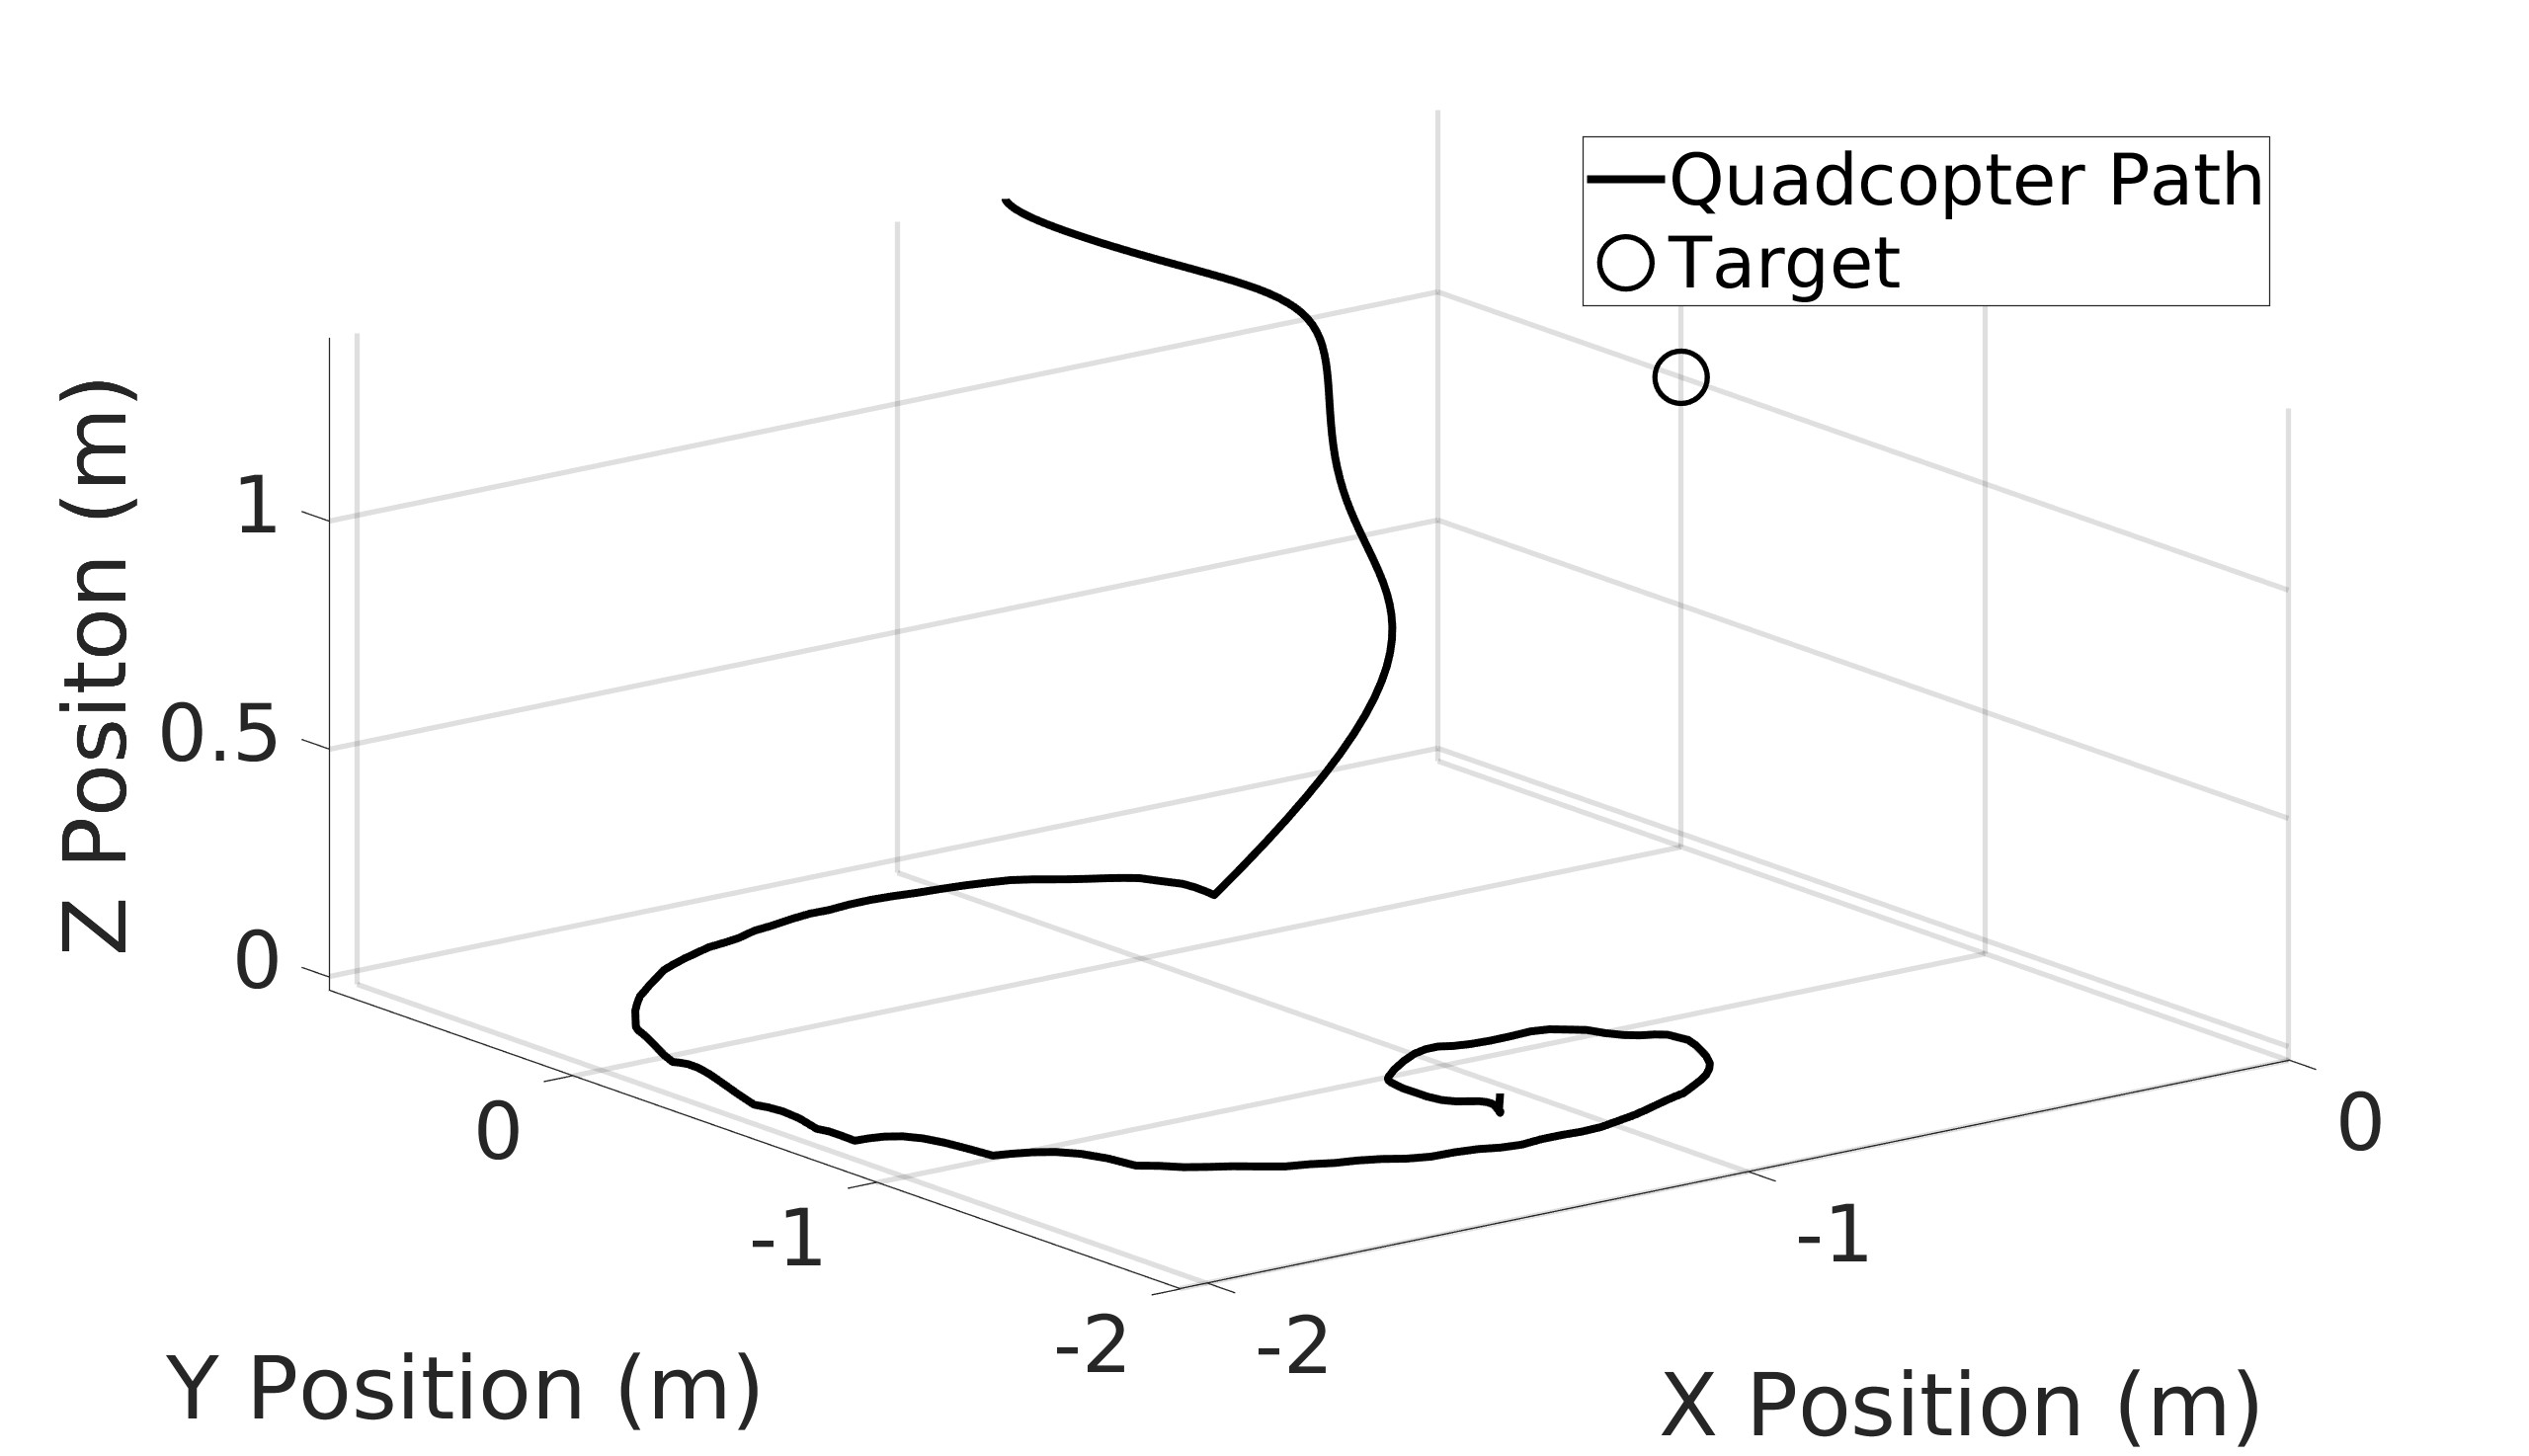
\includegraphics[width=0.735\textwidth]{plots/off_td3_0_5.jpg}
            \caption{Deterministic Path-following Agent Response in Small State Space with the Initial Position of [-0.8, 0.8, 1.4]}
            \label{offT0.5}
    \end{figure}
    Fig. \ref{offS0.5} shows the response of the stochastic agent when starting with an initial position of [-1.5, 1.5, 2]. The stochastic agent successfully stabilized at the target position as shown although the agent was never trained on this point at all. The $x$ and $y$ components are further than the trained state space by 1m and the $z$ component is further by 0.5m.  
    \begin{figure}[H]
            \centering
            \includegraphics[width=0.735\textwidth]{plots/off_SAC_0_5.jpg}
            \caption{Stochastic Path-following Agent Response in Small State Space with the Initial Position of [-1.5, 1.5, 2]}
            \label{offS0.5}
    \end{figure}
Deterministic algorithms train a sample-efficient policy where each state has a single deterministic action. Exploration is done off-policy by adding external noise to the actions. This approach is wasteful and leads to unstable behavior since some regions in the action space close to the current policy are likely to have already been explored by past policies leading to sub-optimal policies \cite{NEURIPS2019_a34bacf8}.
    
 \subsection{Large State Space Training}
In this training, the agents were trained with a larger state space with the same goal to test the ability of each algorithm to learn the entirety of the state space. Both the stochastic training and deterministic training ran for a total of 3,000,000 steps. Fig. \ref{SvT2.5} shows the mean reward obtained by each agent. Both agents obtained the maximum reward at almost the same number of time steps.
\begin{figure}[H]
            \centering
            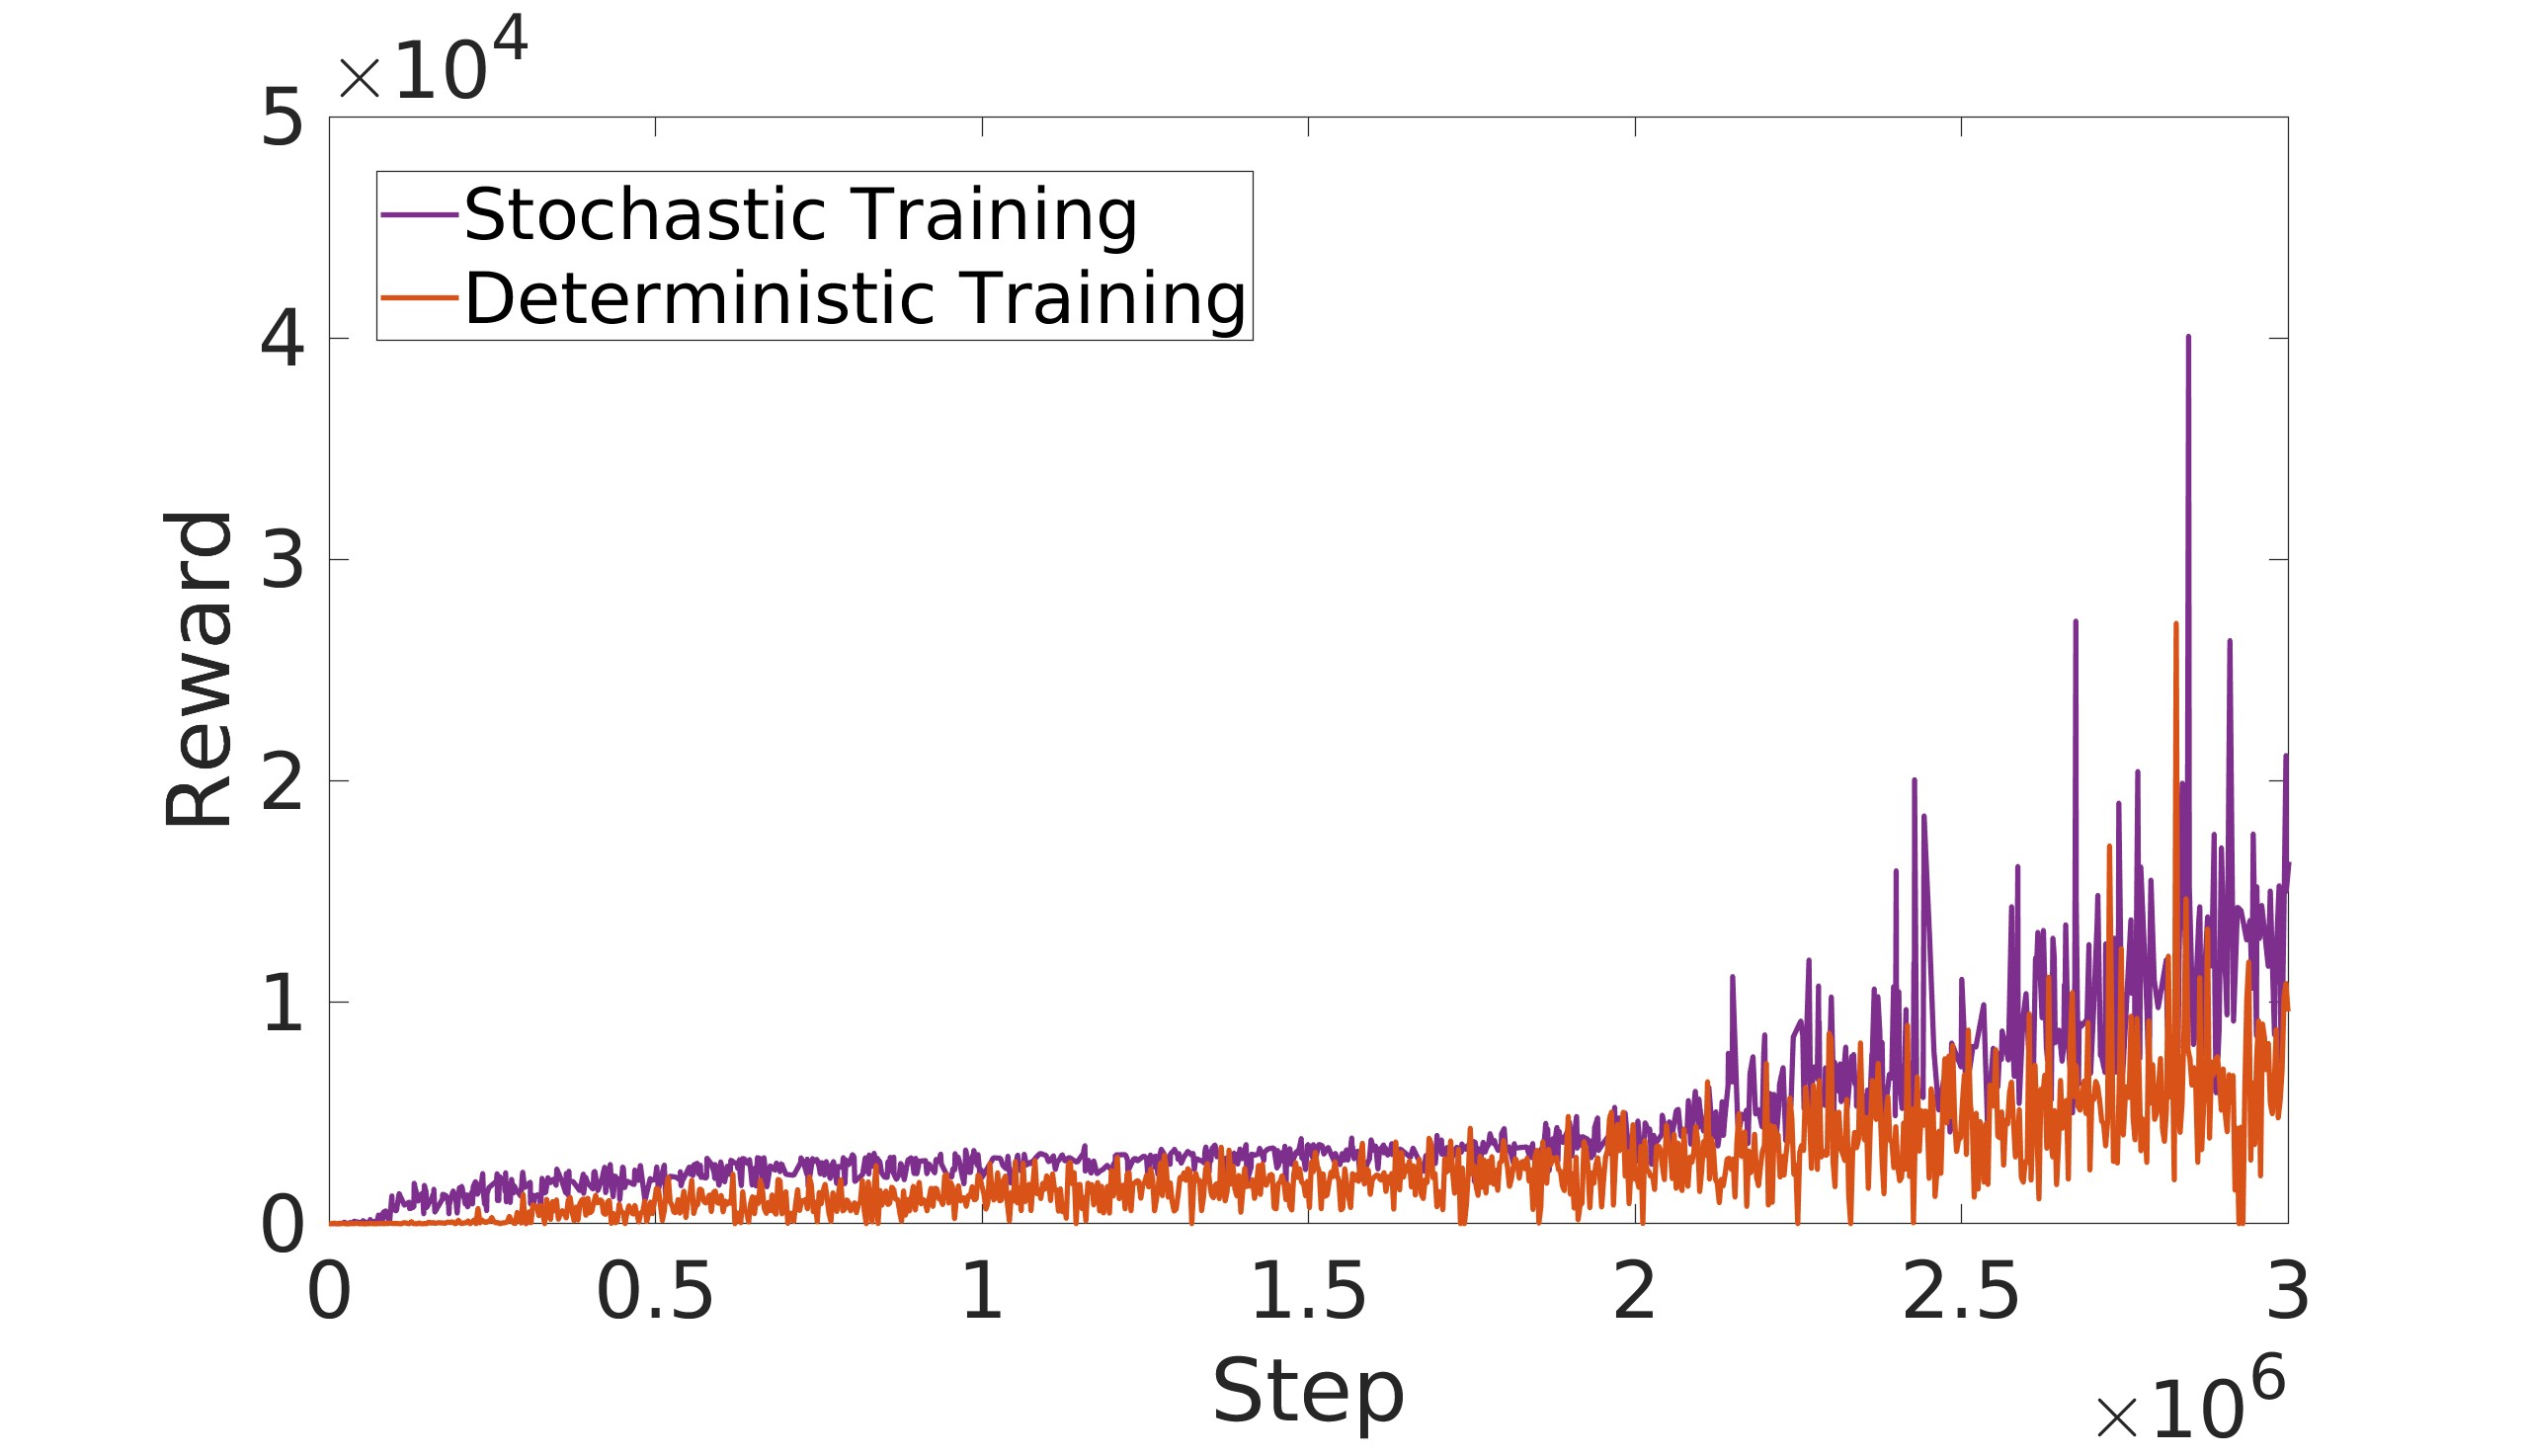
\includegraphics[width=0.8\textwidth]{plots/SACvsTD3_2_5.jpg}
            \caption{Average Mean Reward of Large State Space Training for Deterministic Training and Stochastic Training Algorithms}
            \label{SvT2.5}
    \end{figure}\clearpage

Fig. \ref{x2.5} shows the stochastic agent response when starting from an initial position of [-1.5, 1.5, 1.5] compared to the deterministic agent response. This point was chosen as a close position to the target. Both agents stabilized with zero steady-state errors. As shown the performance of both agents again is almost identical with negligible differences between the two algorithms.
\begin{figure}[H]
            \centering
            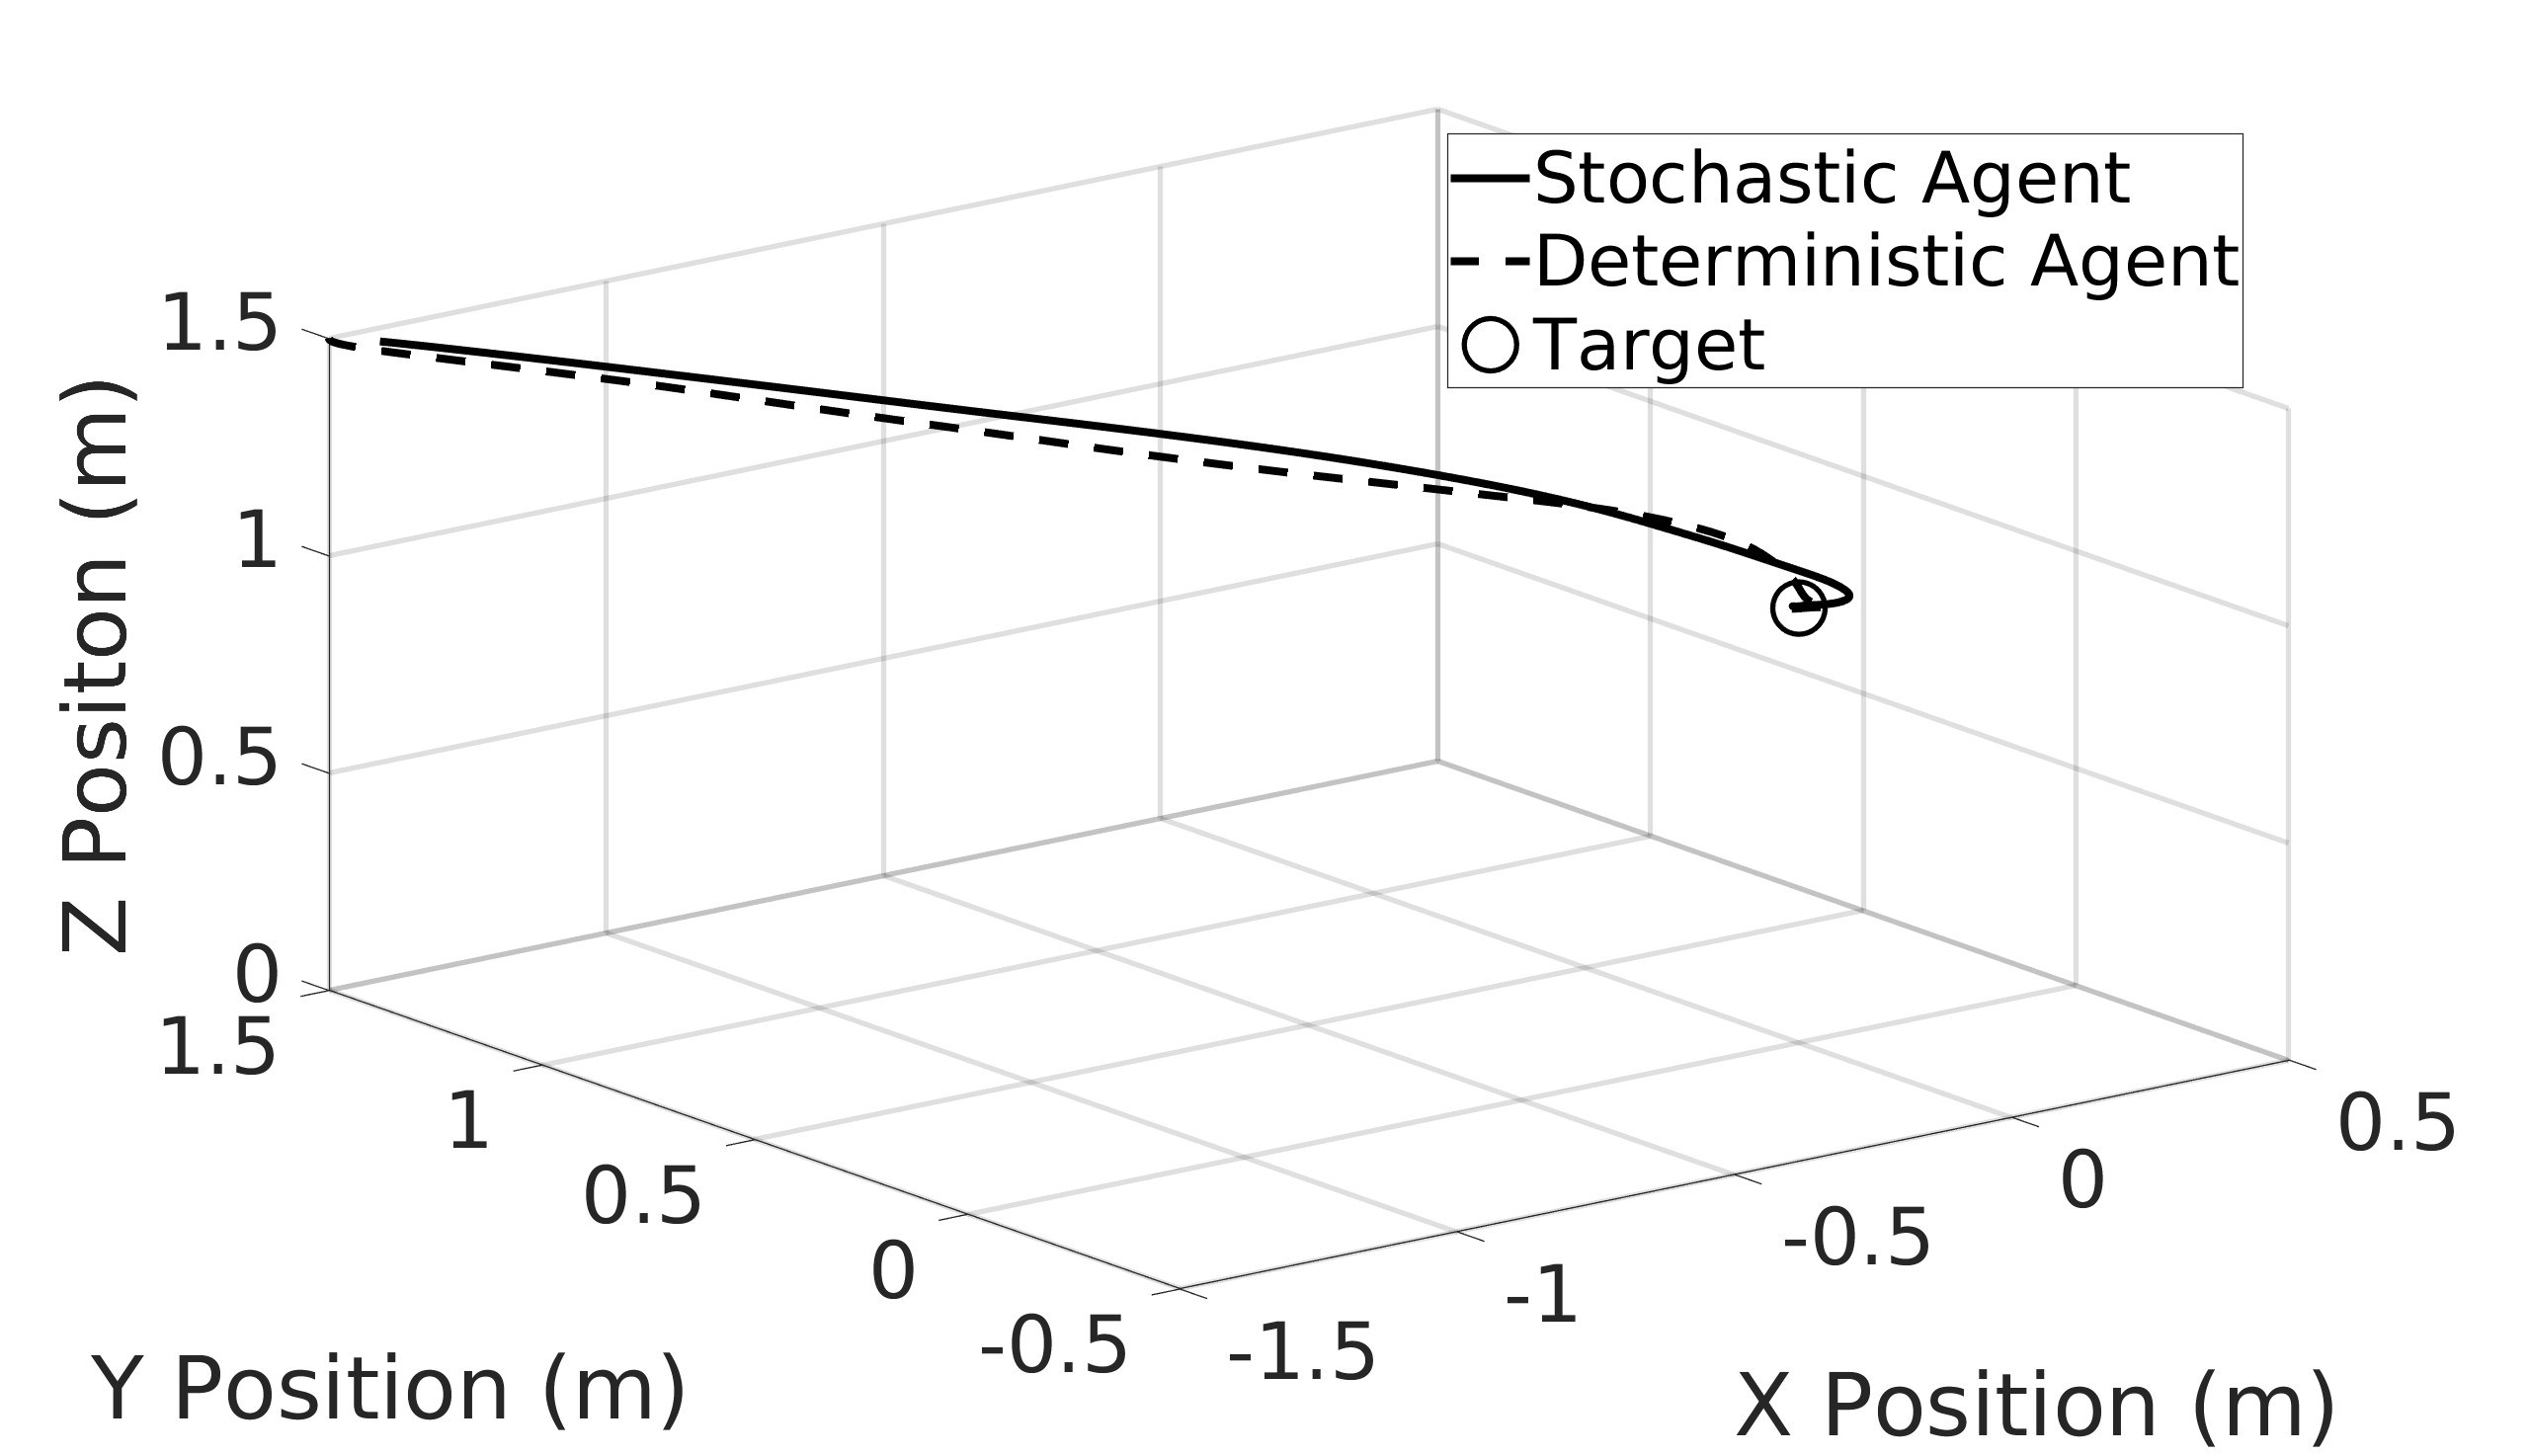
\includegraphics[width=0.695\textwidth]{plots/1_5_1.jpg}
            \caption{Large State Space Response of an Initial Position of [-1.5, 1.5, 1.5] for Deterministic and Stochastic Agents}
            \label{x2.5}
    \end{figure}
    However, when passing the most extreme point both agents were trained on, point [-2.5, 2.5, 2.5], the deterministic agent crashes and fails to reach the target as shown in Fig. \ref{T2.5}. This shows that the deterministic agent failed to learn the entirety of the state space in time. 
    \begin{figure}[H]
            \centering
            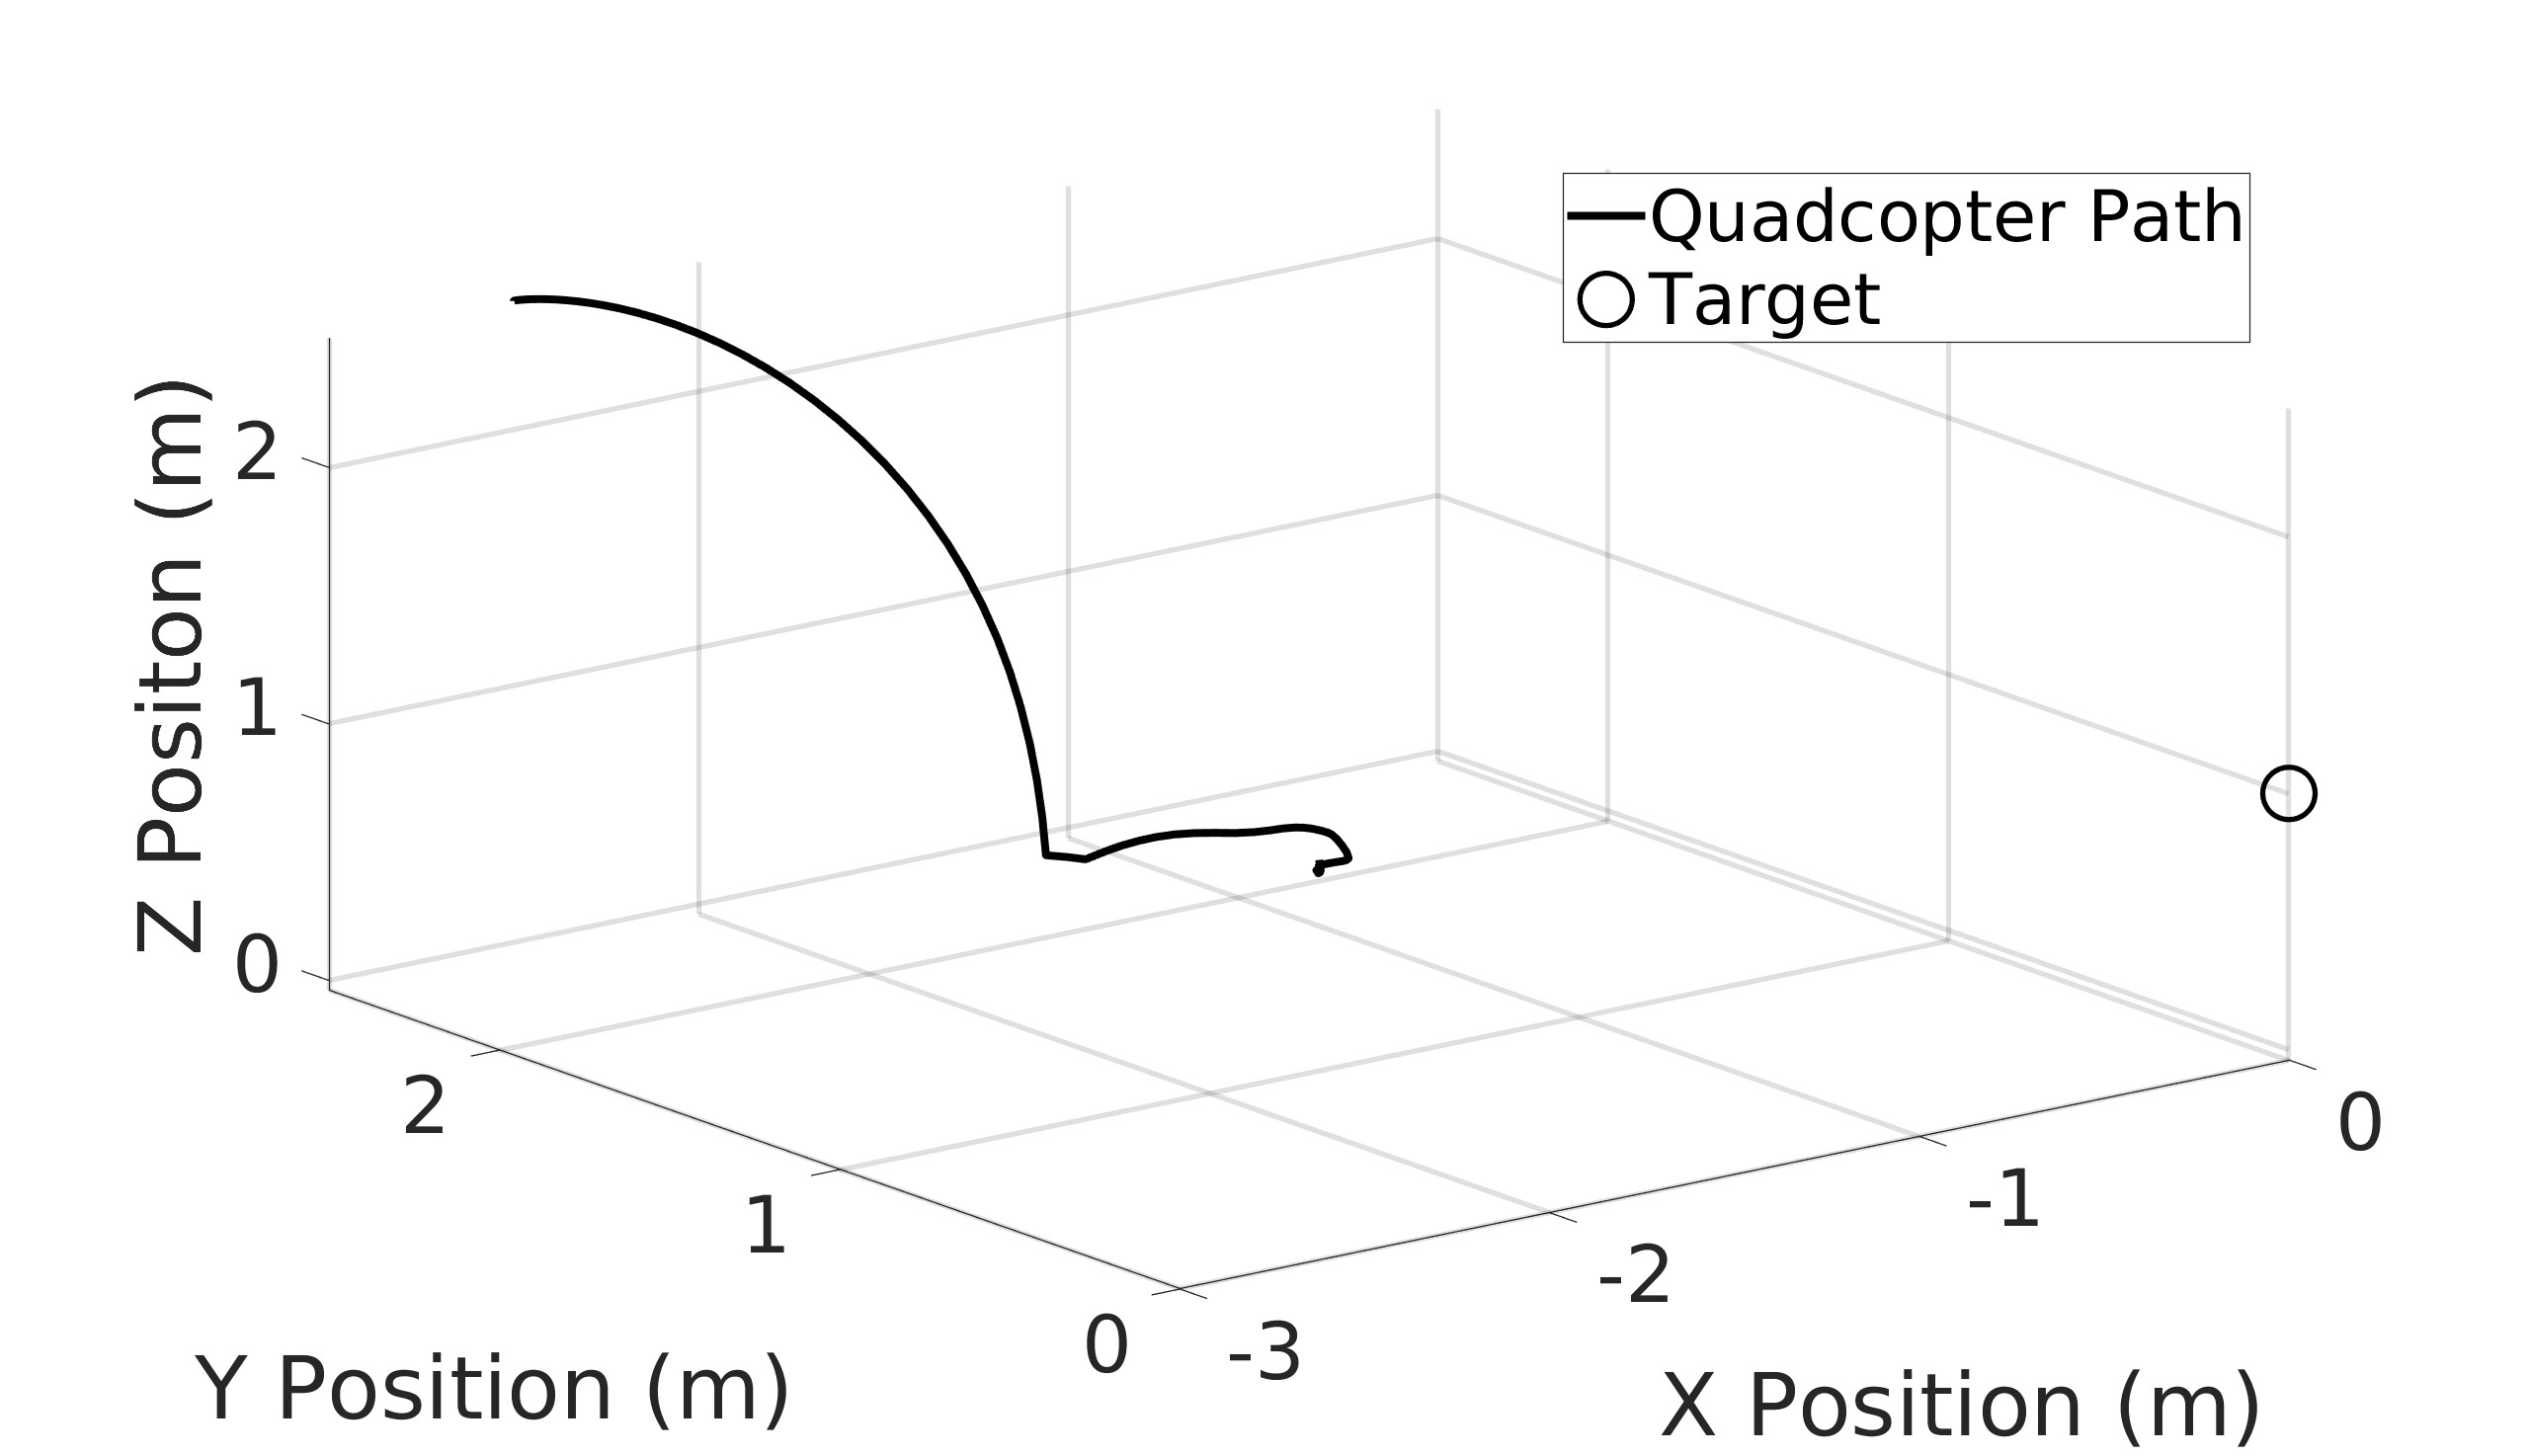
\includegraphics[width=0.695\textwidth]{plots/2_5_crash.jpg}
            \caption{Path-following Response of Deterministic Agent in Large State Space for an Initial Position of [-2.5, 2.5, 2.5]}
            \label{T2.5}
    \end{figure}
    Fig. \ref{S2.5} shows the response of the stochastic training agent when starting with an initial position of [-2.5, 2.5, 2.5]. The stochastic training agent successfully stabilized at the target position as shown. This shows that the stochastic training agent was able to learn the entirety of the state space. 
    \begin{figure}[H]
            \centering
            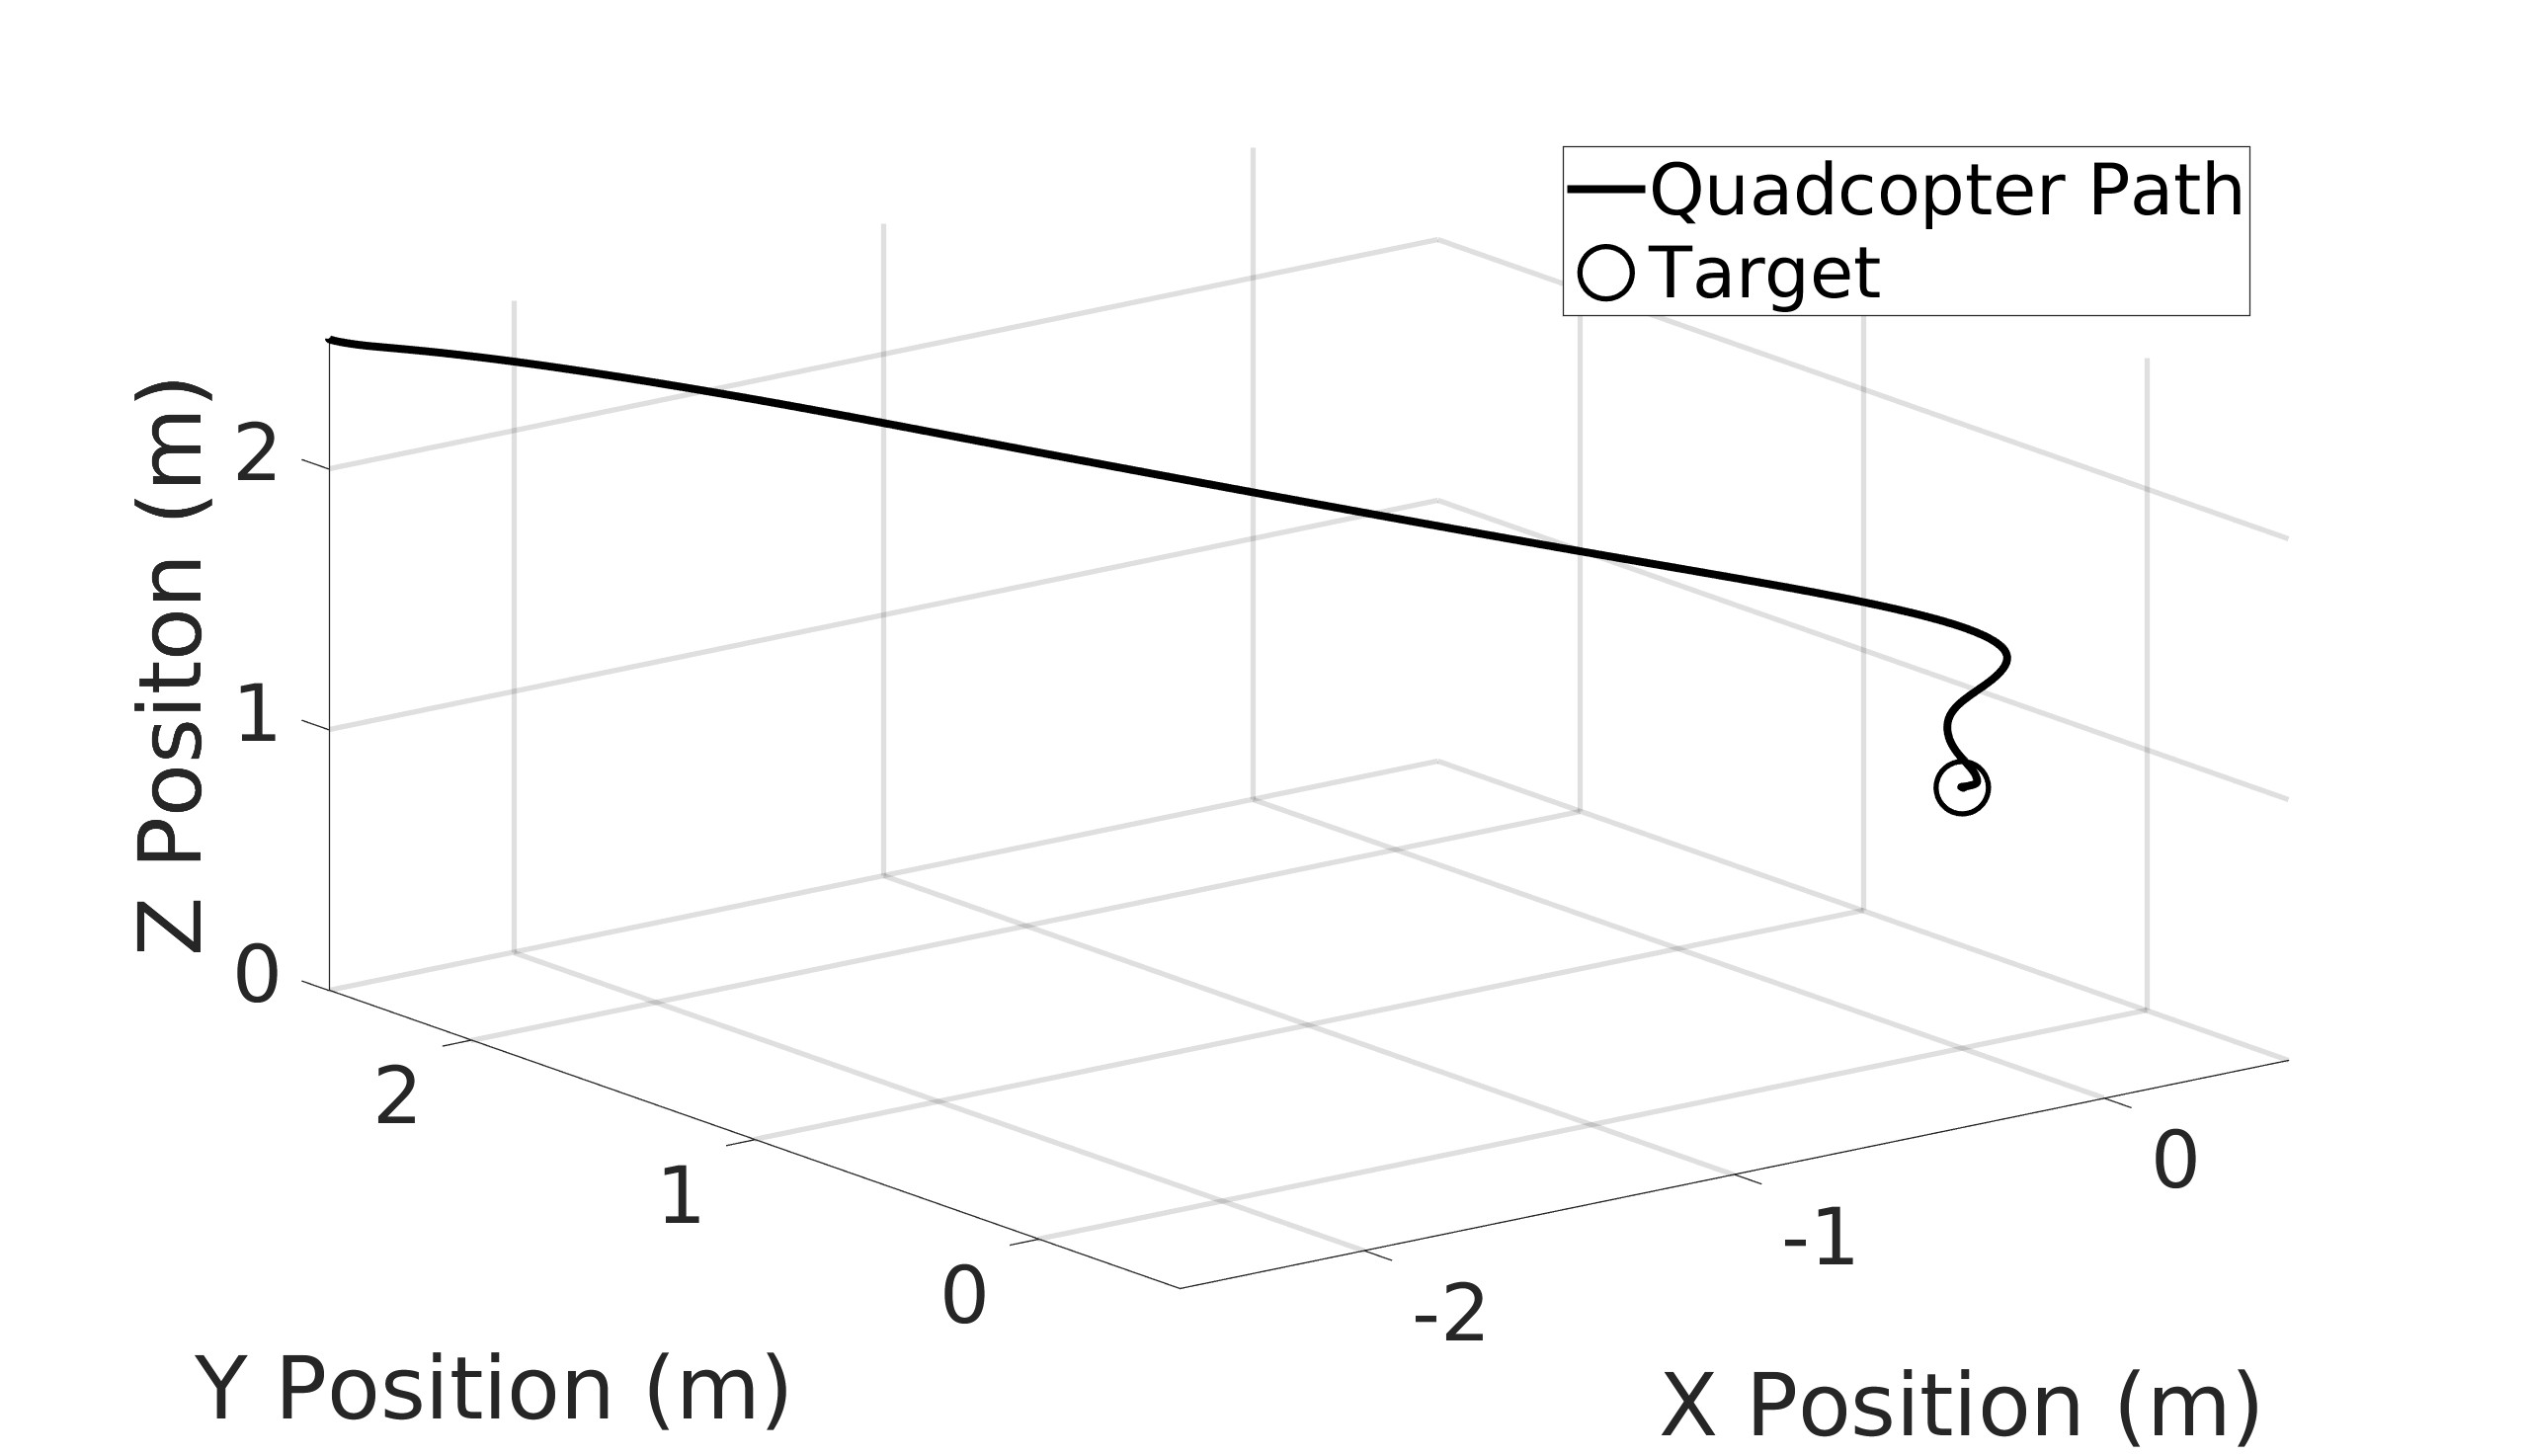
\includegraphics[width=0.735\textwidth]{plots/2_5_1.jpg}
            \caption{Path-following Response of Stochastic Agent in Large State Space for an Initial Position of [-2.5, 2.5, 2.5]}
            \label{S2.5}
    \end{figure}
    In contrast to deterministic algorithms, stochastic algorithms train a sample-efficient policy where each observation has a probability distribution over actions to maximize the potential reward. By adding an entropy term to the policy parameters along with the reward, stochastic algorithms encourage exploration while maximizing the rewards promoting a balance between exploration and exploitation leading to a more stable algorithm \cite{haarnoja2018soft}. Higher entropy results in more stochasticity, preventing the policy from collapsing into determinism. This explains the ability of the stochastic algorithm to learn the entirety of the state space faster than the deterministic algorithm.
    \clearpage
   Fig. \ref{offS4.5} shows the response of the stochastic training agent when starting with an initial position of [3.5, 3.5, 3]. The stochastic training agent successfully stabilized at the target position as shown although the agent was never trained on this point previously. 
    \begin{figure}[H]
            \centering
            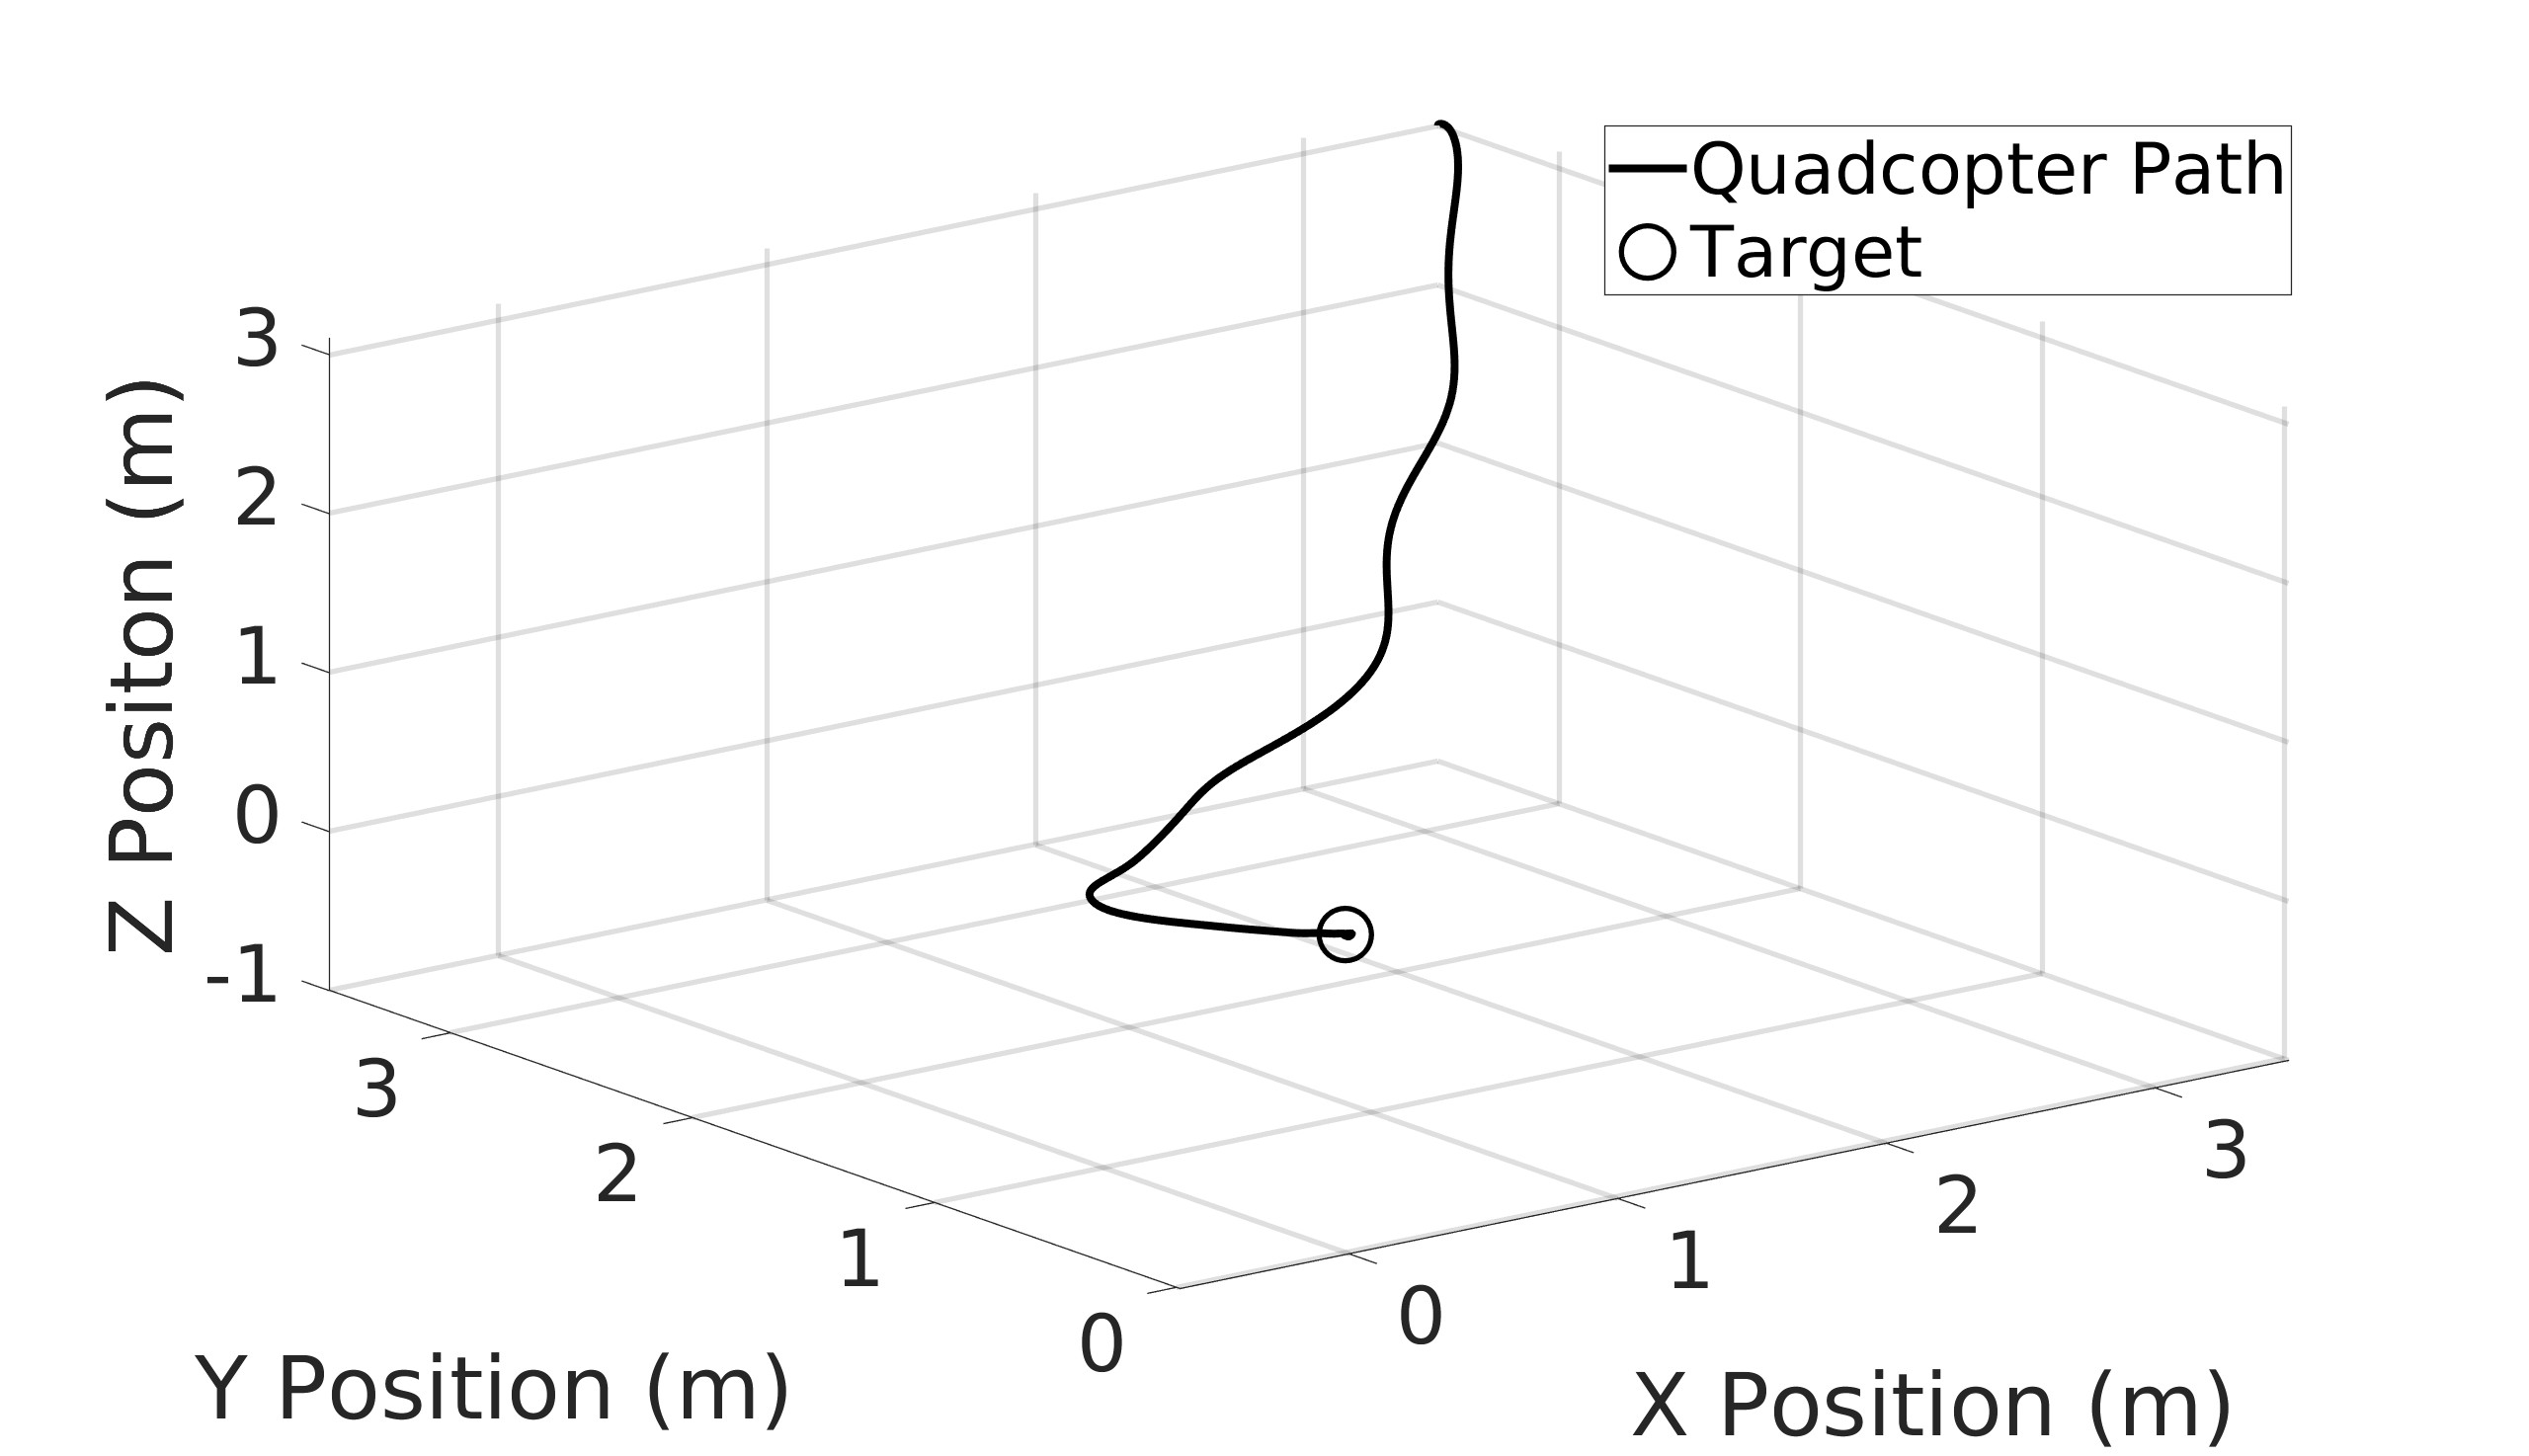
\includegraphics[width=0.735\textwidth]{plots/off_sac_2_5.jpg}
            \caption{Path-following Response of Stochastic Agent in Large State Space for an Initial Position of [3.5, 3.5, 3]}
            \label{offS4.5}
    \end{figure}
    Not only did the stochastic agent learn the entirety of the state space, but also the stochastic agent successfully reached the target when presented with an initial position outside the trained state space. Dynamic entropy tuning in stochastic algorithms optimizes the entropy coefficient online, allowing the algorithm to learn when to explore and when to exploit. This explains why stochastic algorithm can predict correct actions when presented with states outside its training data. \clearpage
\section{Position Controller Training}
The objective of this training was the same as the path-following agent to stabilize the quadcopter at the same point as quickly as possible. 2-D plots are used in this section to highlight the performance difference between the two agents. Fig. \ref{deterministic trainingrew} shows the mean reward obtained by the deterministic training agent. The agent was trained for a total of 4,827,000 steps with the maximum reward  of of 5,000 as shown. Catastrophic forgetting of the optimal policy starts to appear as after reaching the optimal policy the agent's response starts worsening.
    \begin{figure}[H]
            \centering
            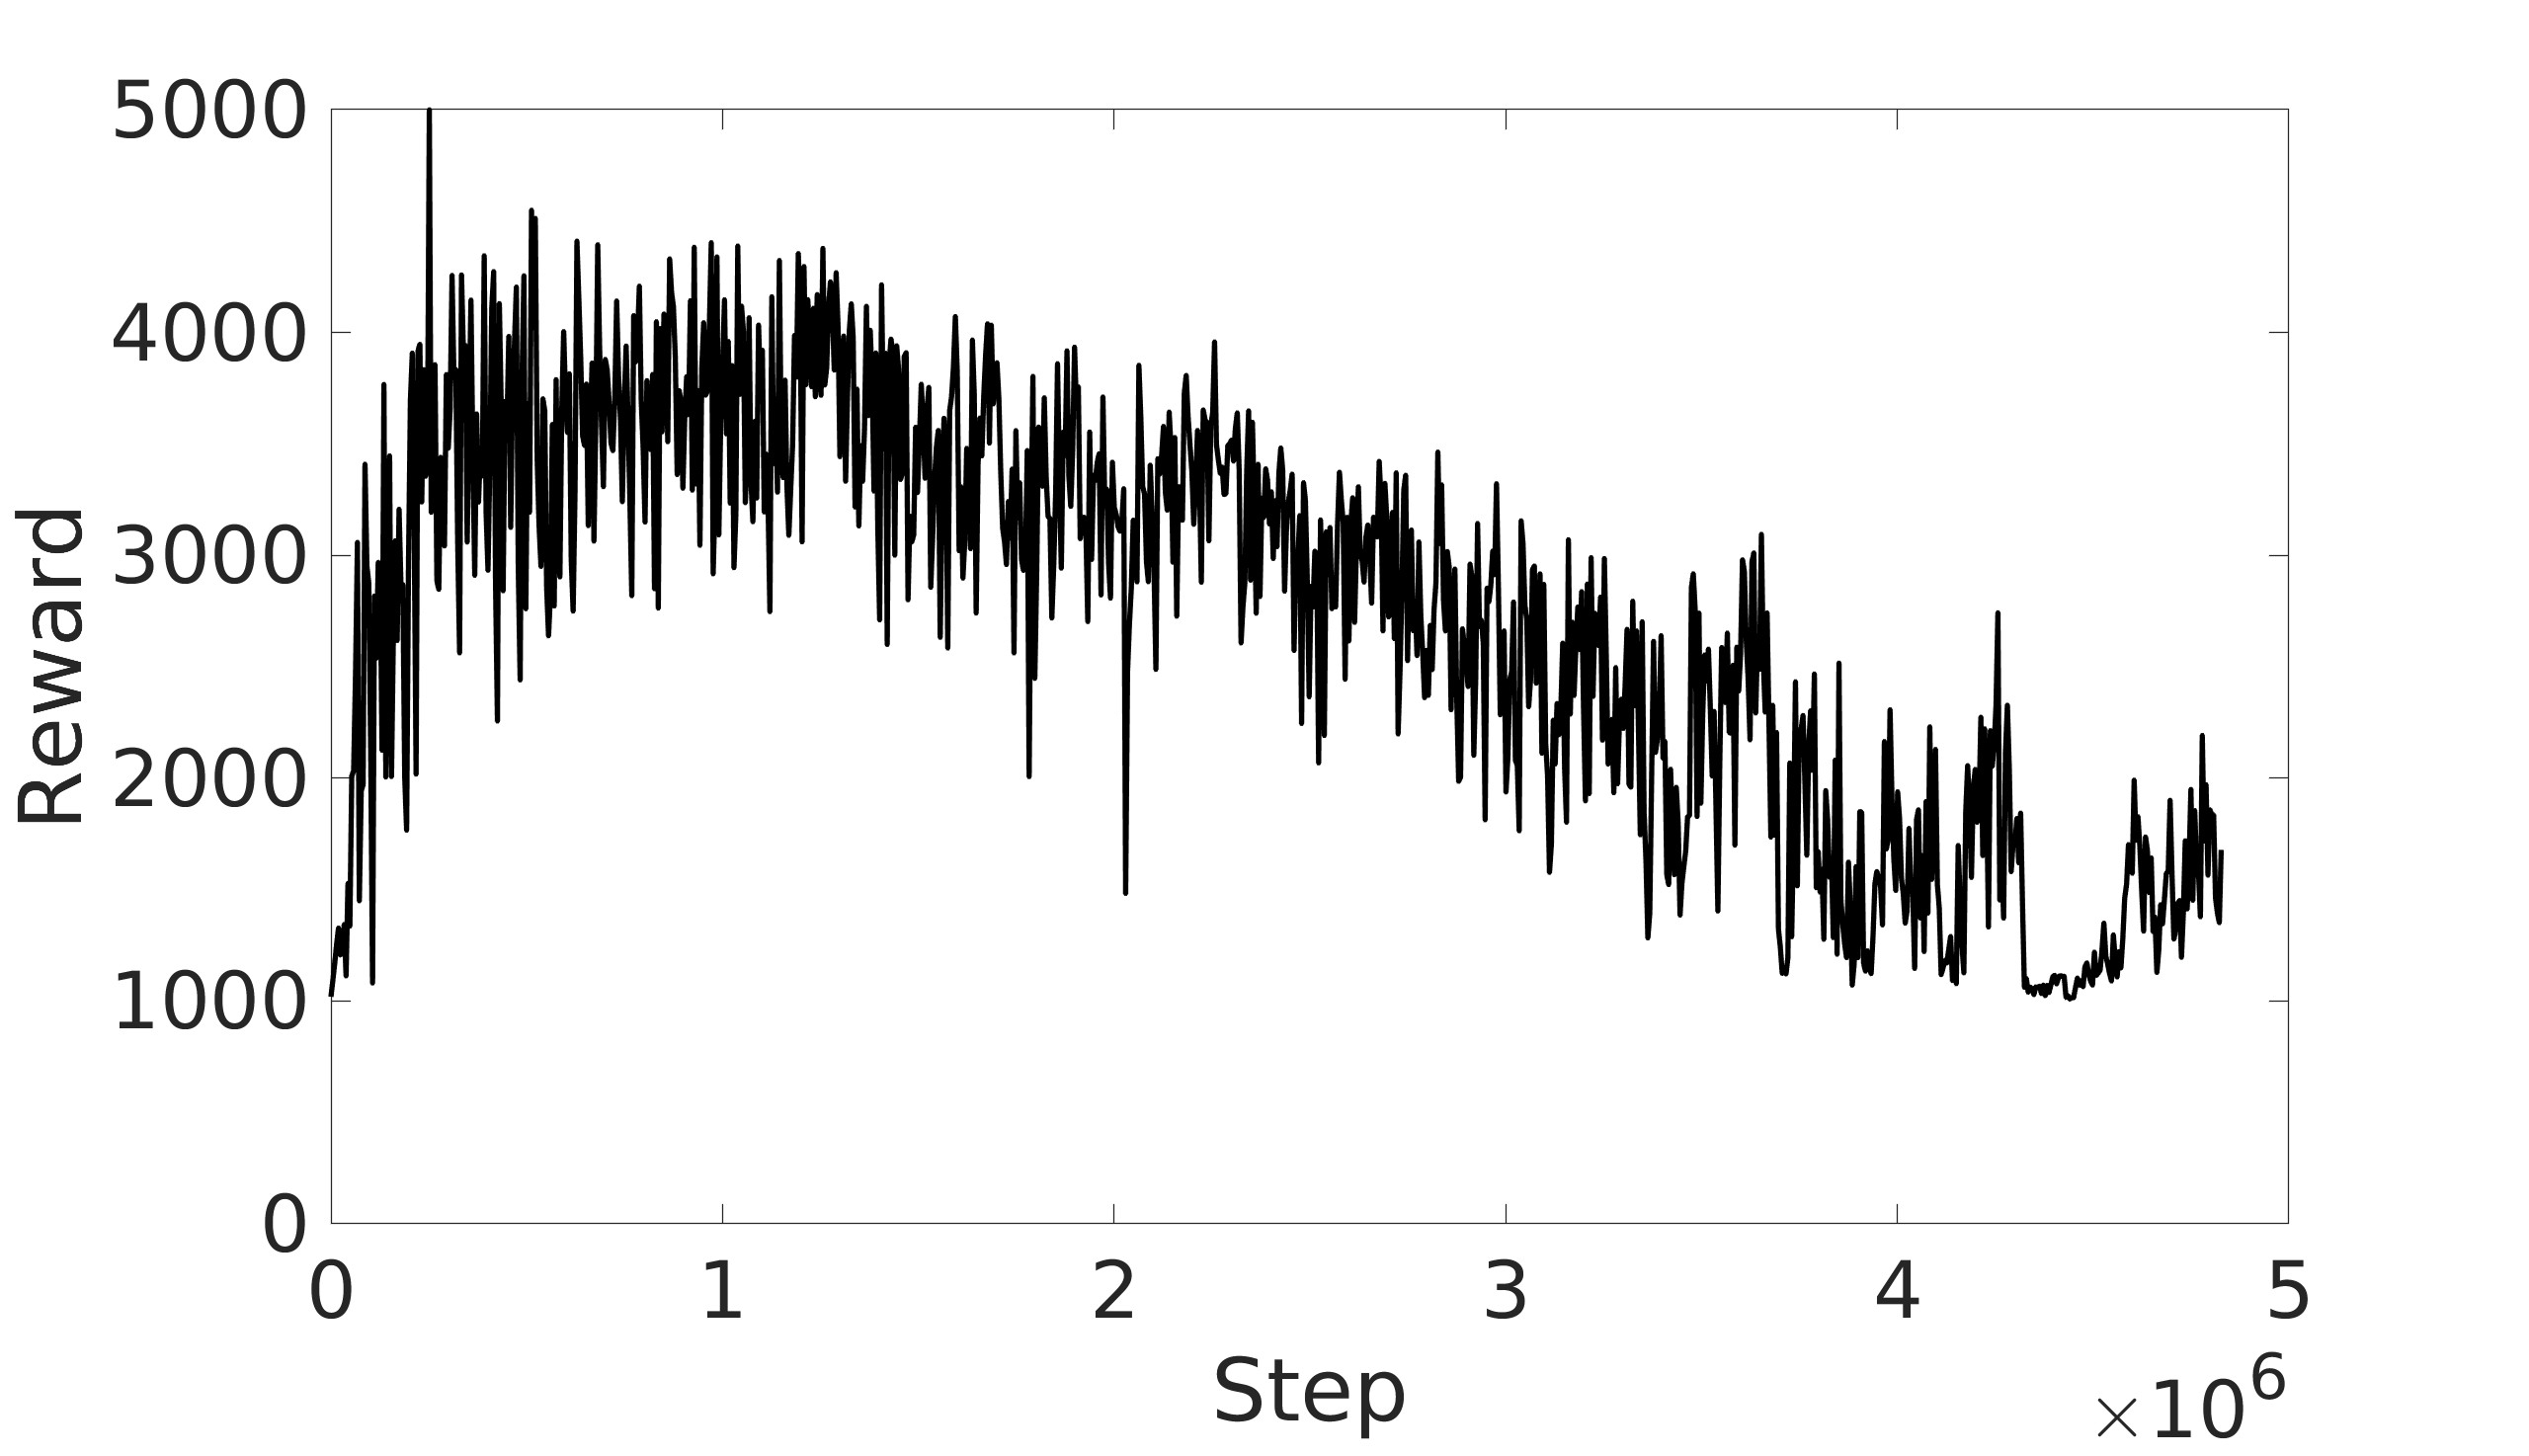
\includegraphics[width=0.75\textwidth]{plots/td3_rew.jpg}
            \caption{Mean Reward for the Stabilization Training of Deterministic Position Controller}
            \label{deterministic trainingrew}
    \end{figure}
    Deterministic algorithms gradually worsen after a peak performance as learning continues, this might occur since with a better policy, experiences that have never occurred in the system before are discovered \cite{lu2020adaptive}.
    
Fig. \ref{stbrew} shows the mean reward obtained by the stochastic training agent. The agent was trained for the same number of steps with the maximum reward reached at the 2,978,500 step with a value of 135,023 as shown. This is 130,00 more than the maximum of the deterministic training. Catastrophic forgetting started to appear after reaching the optimal policy. However, in the stochastic algorithm, the dynamic entropy tuning helped the algorithm recover from it.
 \begin{figure}[H]
            \centering
            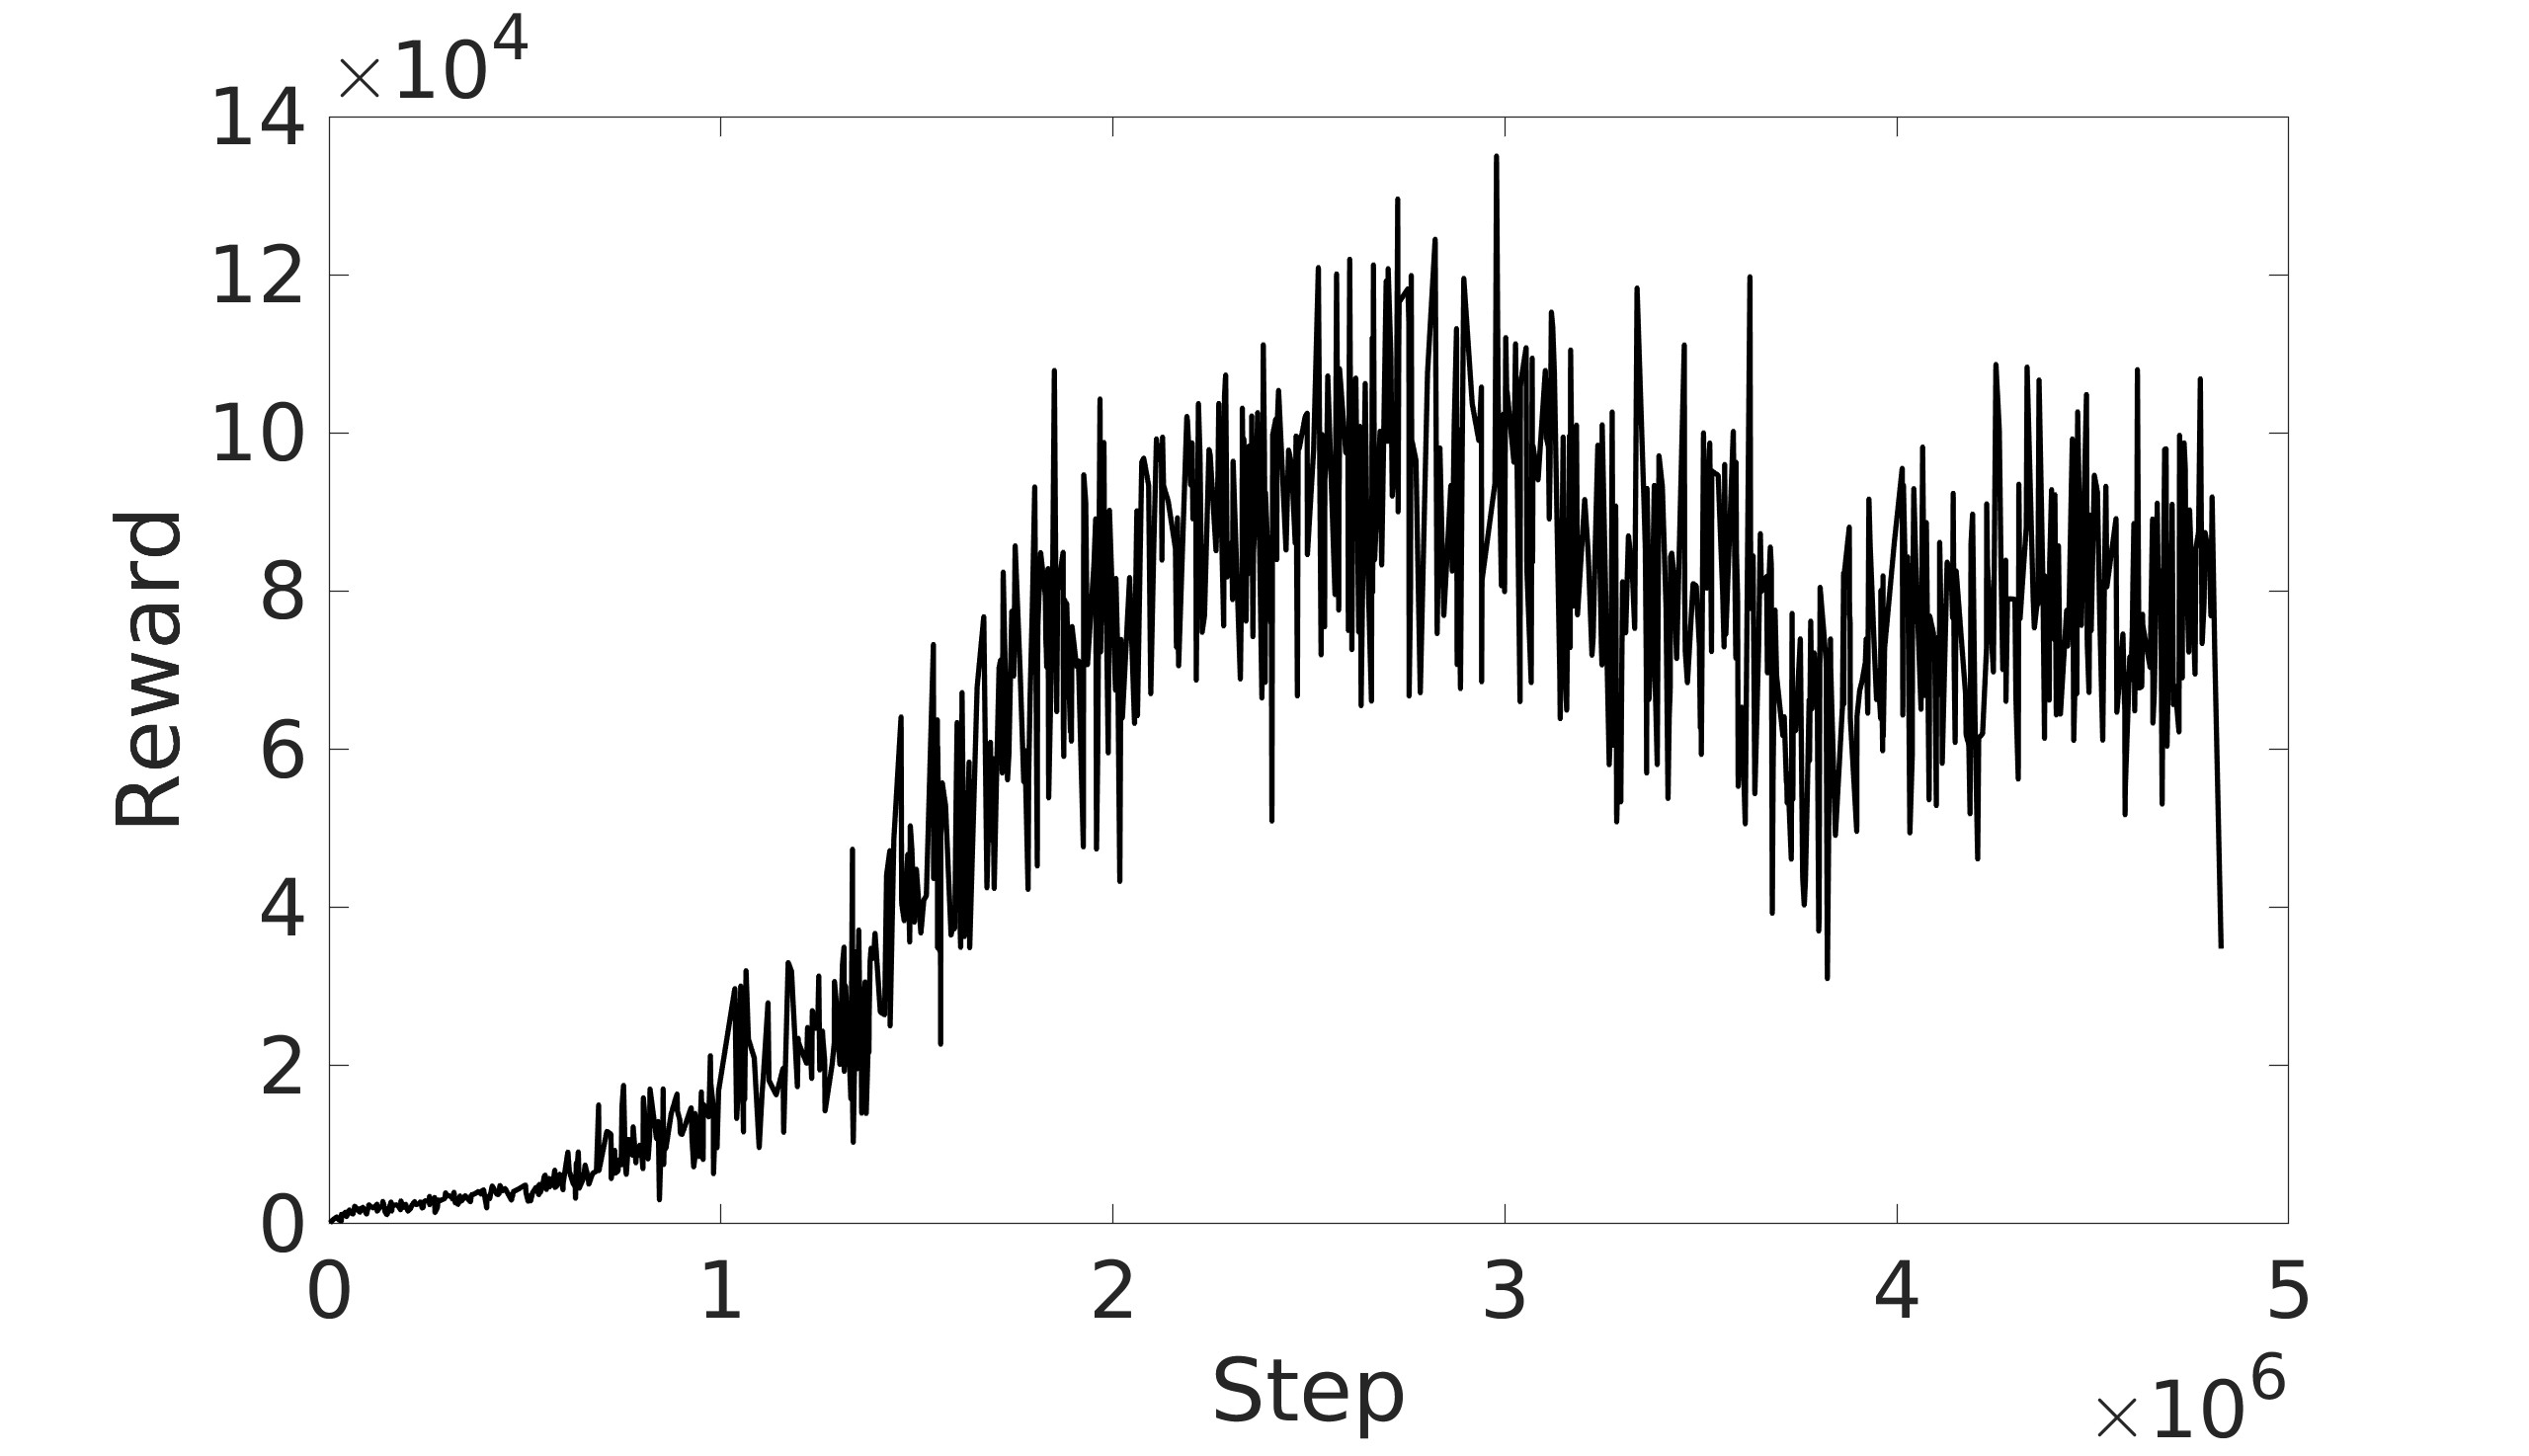
\includegraphics[width=0.75\textwidth]{plots/stab_rew.jpg}
            \caption{Mean Reward for the Stabilization Training of Stochastic Position Controller}
            \label{stbrew}
    \end{figure}
   
   Starting from an initial position of [0.4, 0.8, 0.5], for the $x$-axis response, the stochastic training agent stabilized with zero steady-state, zero overshoot and a settling time of 2.5 seconds. The deterministic training agent on the other hand failed to stabilize as shown in Fig. \ref{X1}.
    \begin{figure}[H]
            \centering
            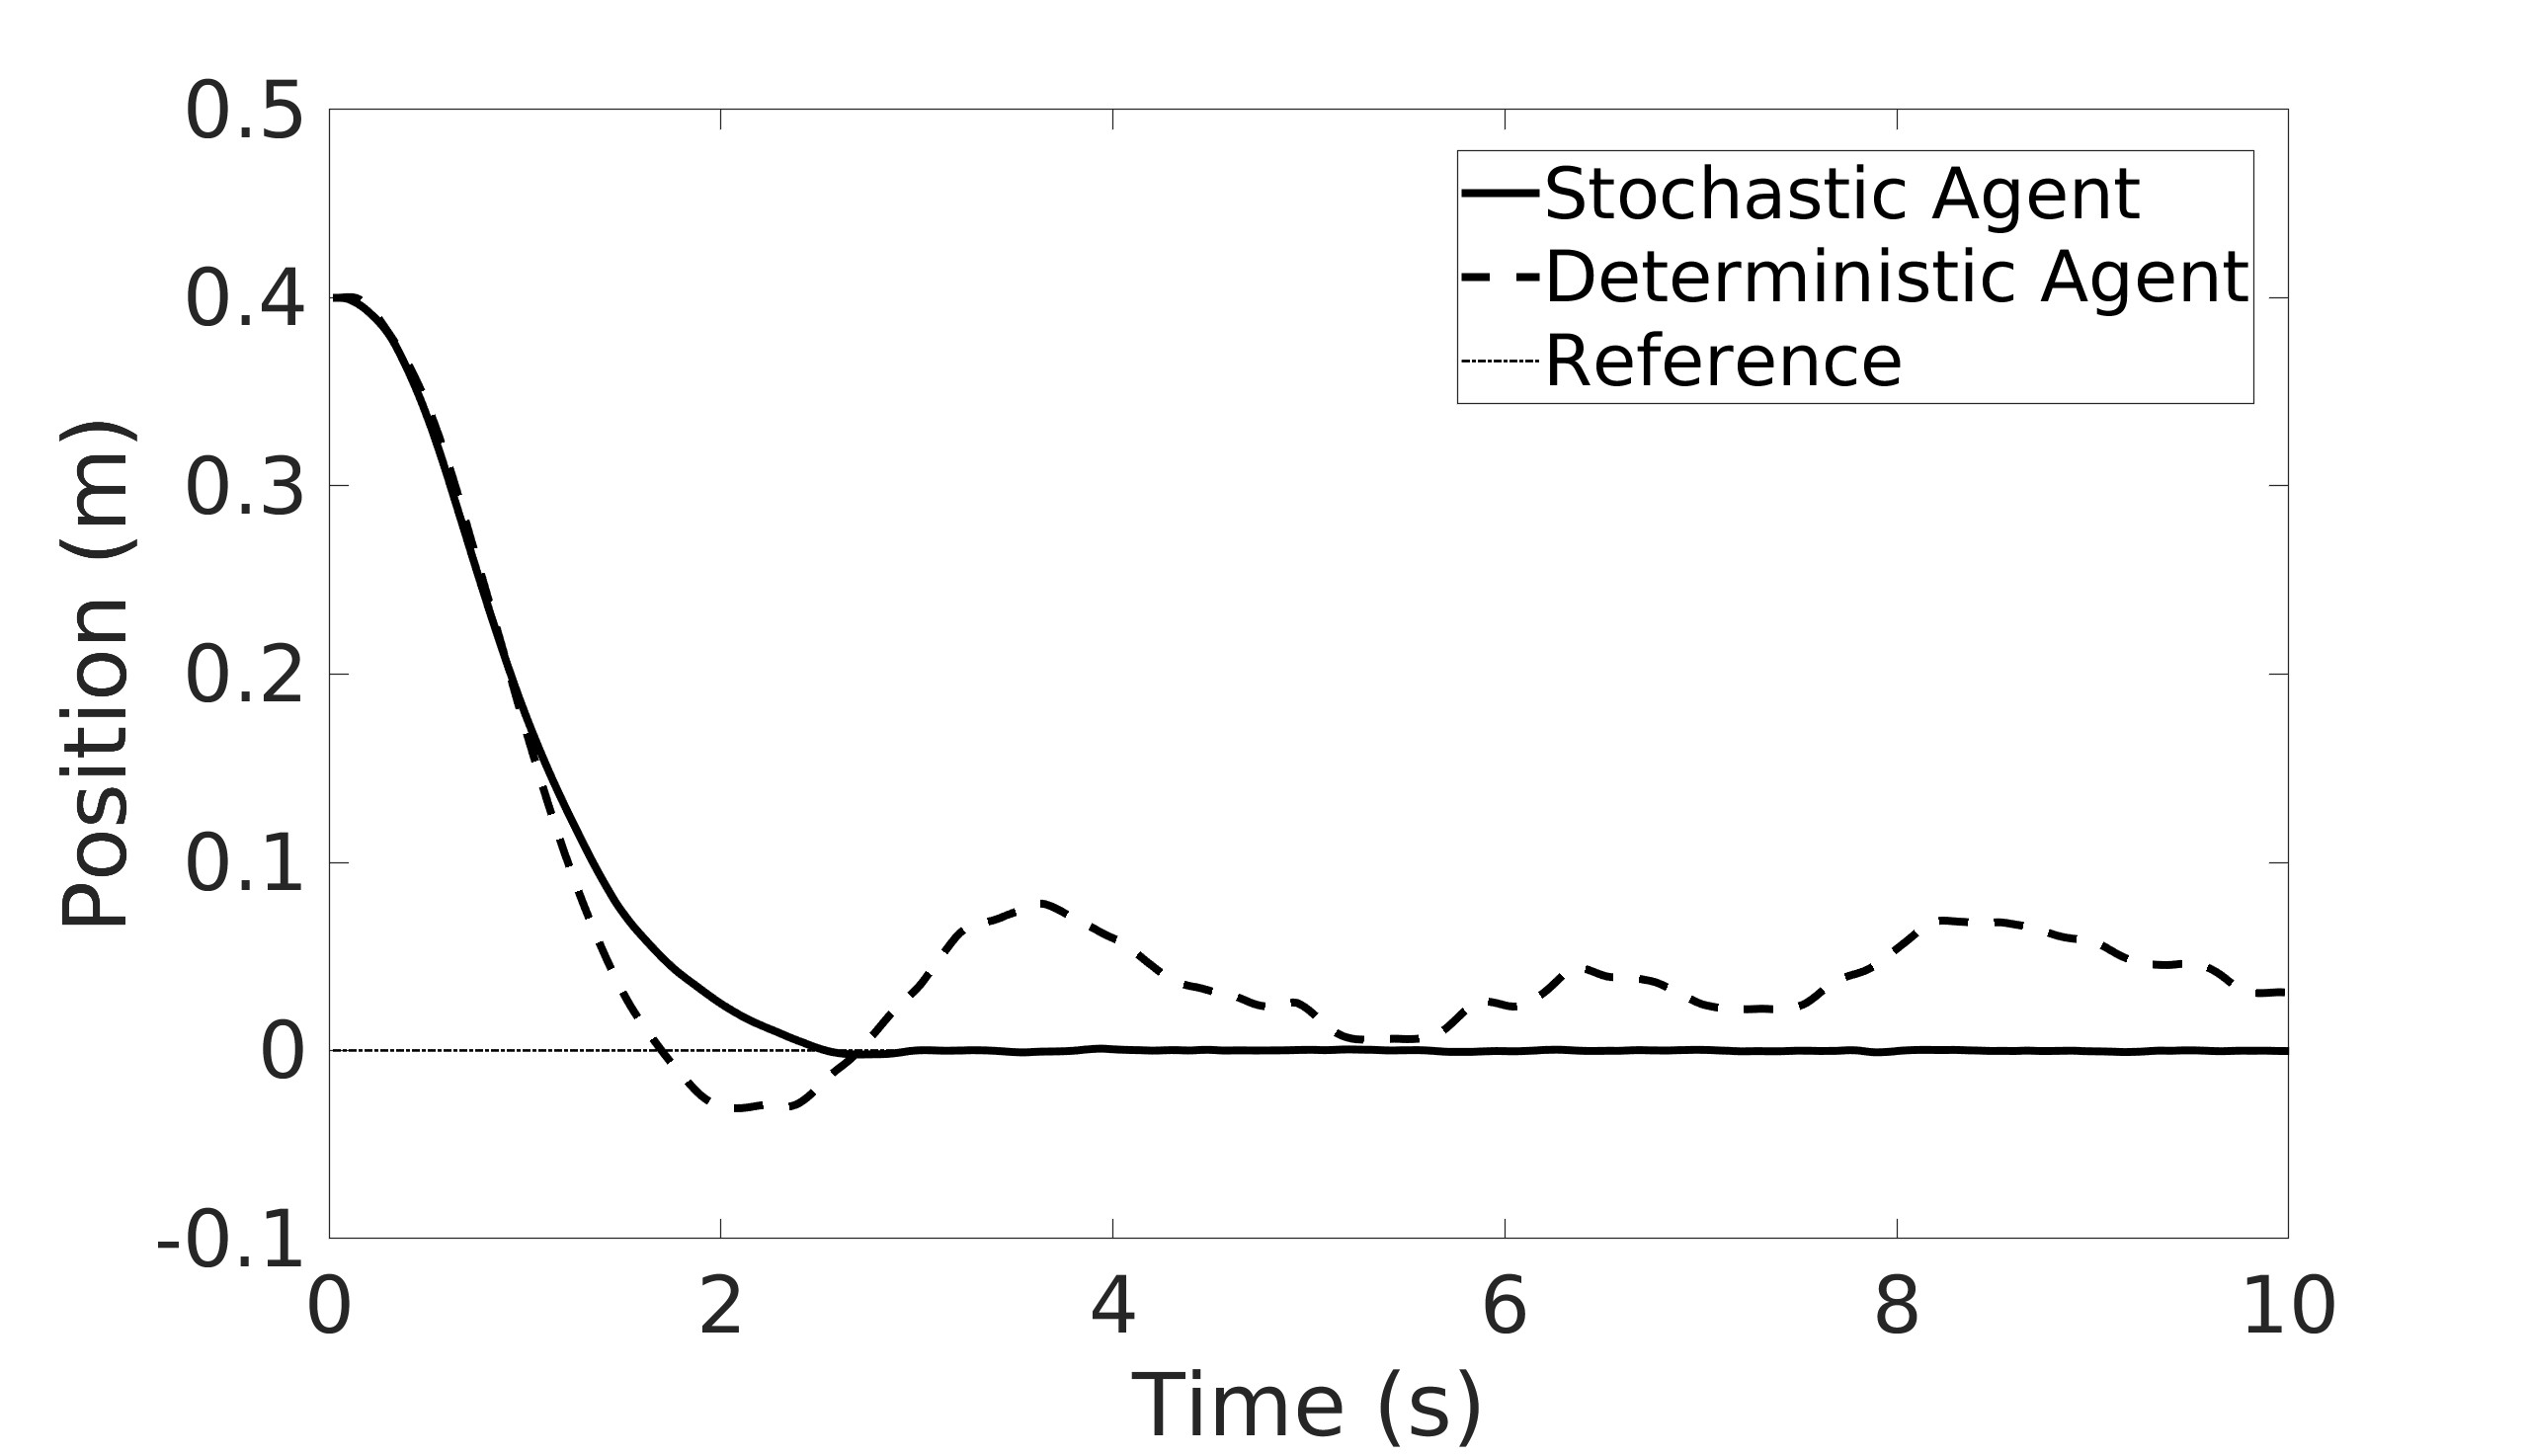
\includegraphics[width=0.75\textwidth]{plots/x1.jpg}
            \caption{$x$-axis Response for an Initial Position of 0.4 for Deterministic and Stochastic Position Controllers}
            \label{X1}
    \end{figure}\clearpage
    For the $y$-axis response in Fig. \ref{y1}, the stochastic training agent stabilized with zero steady-state, zero overshoot and a settling time of 2.5 seconds. The deterministic training agent on the other hand oscillates around the output.
    \begin{figure}[H]
            \centering
            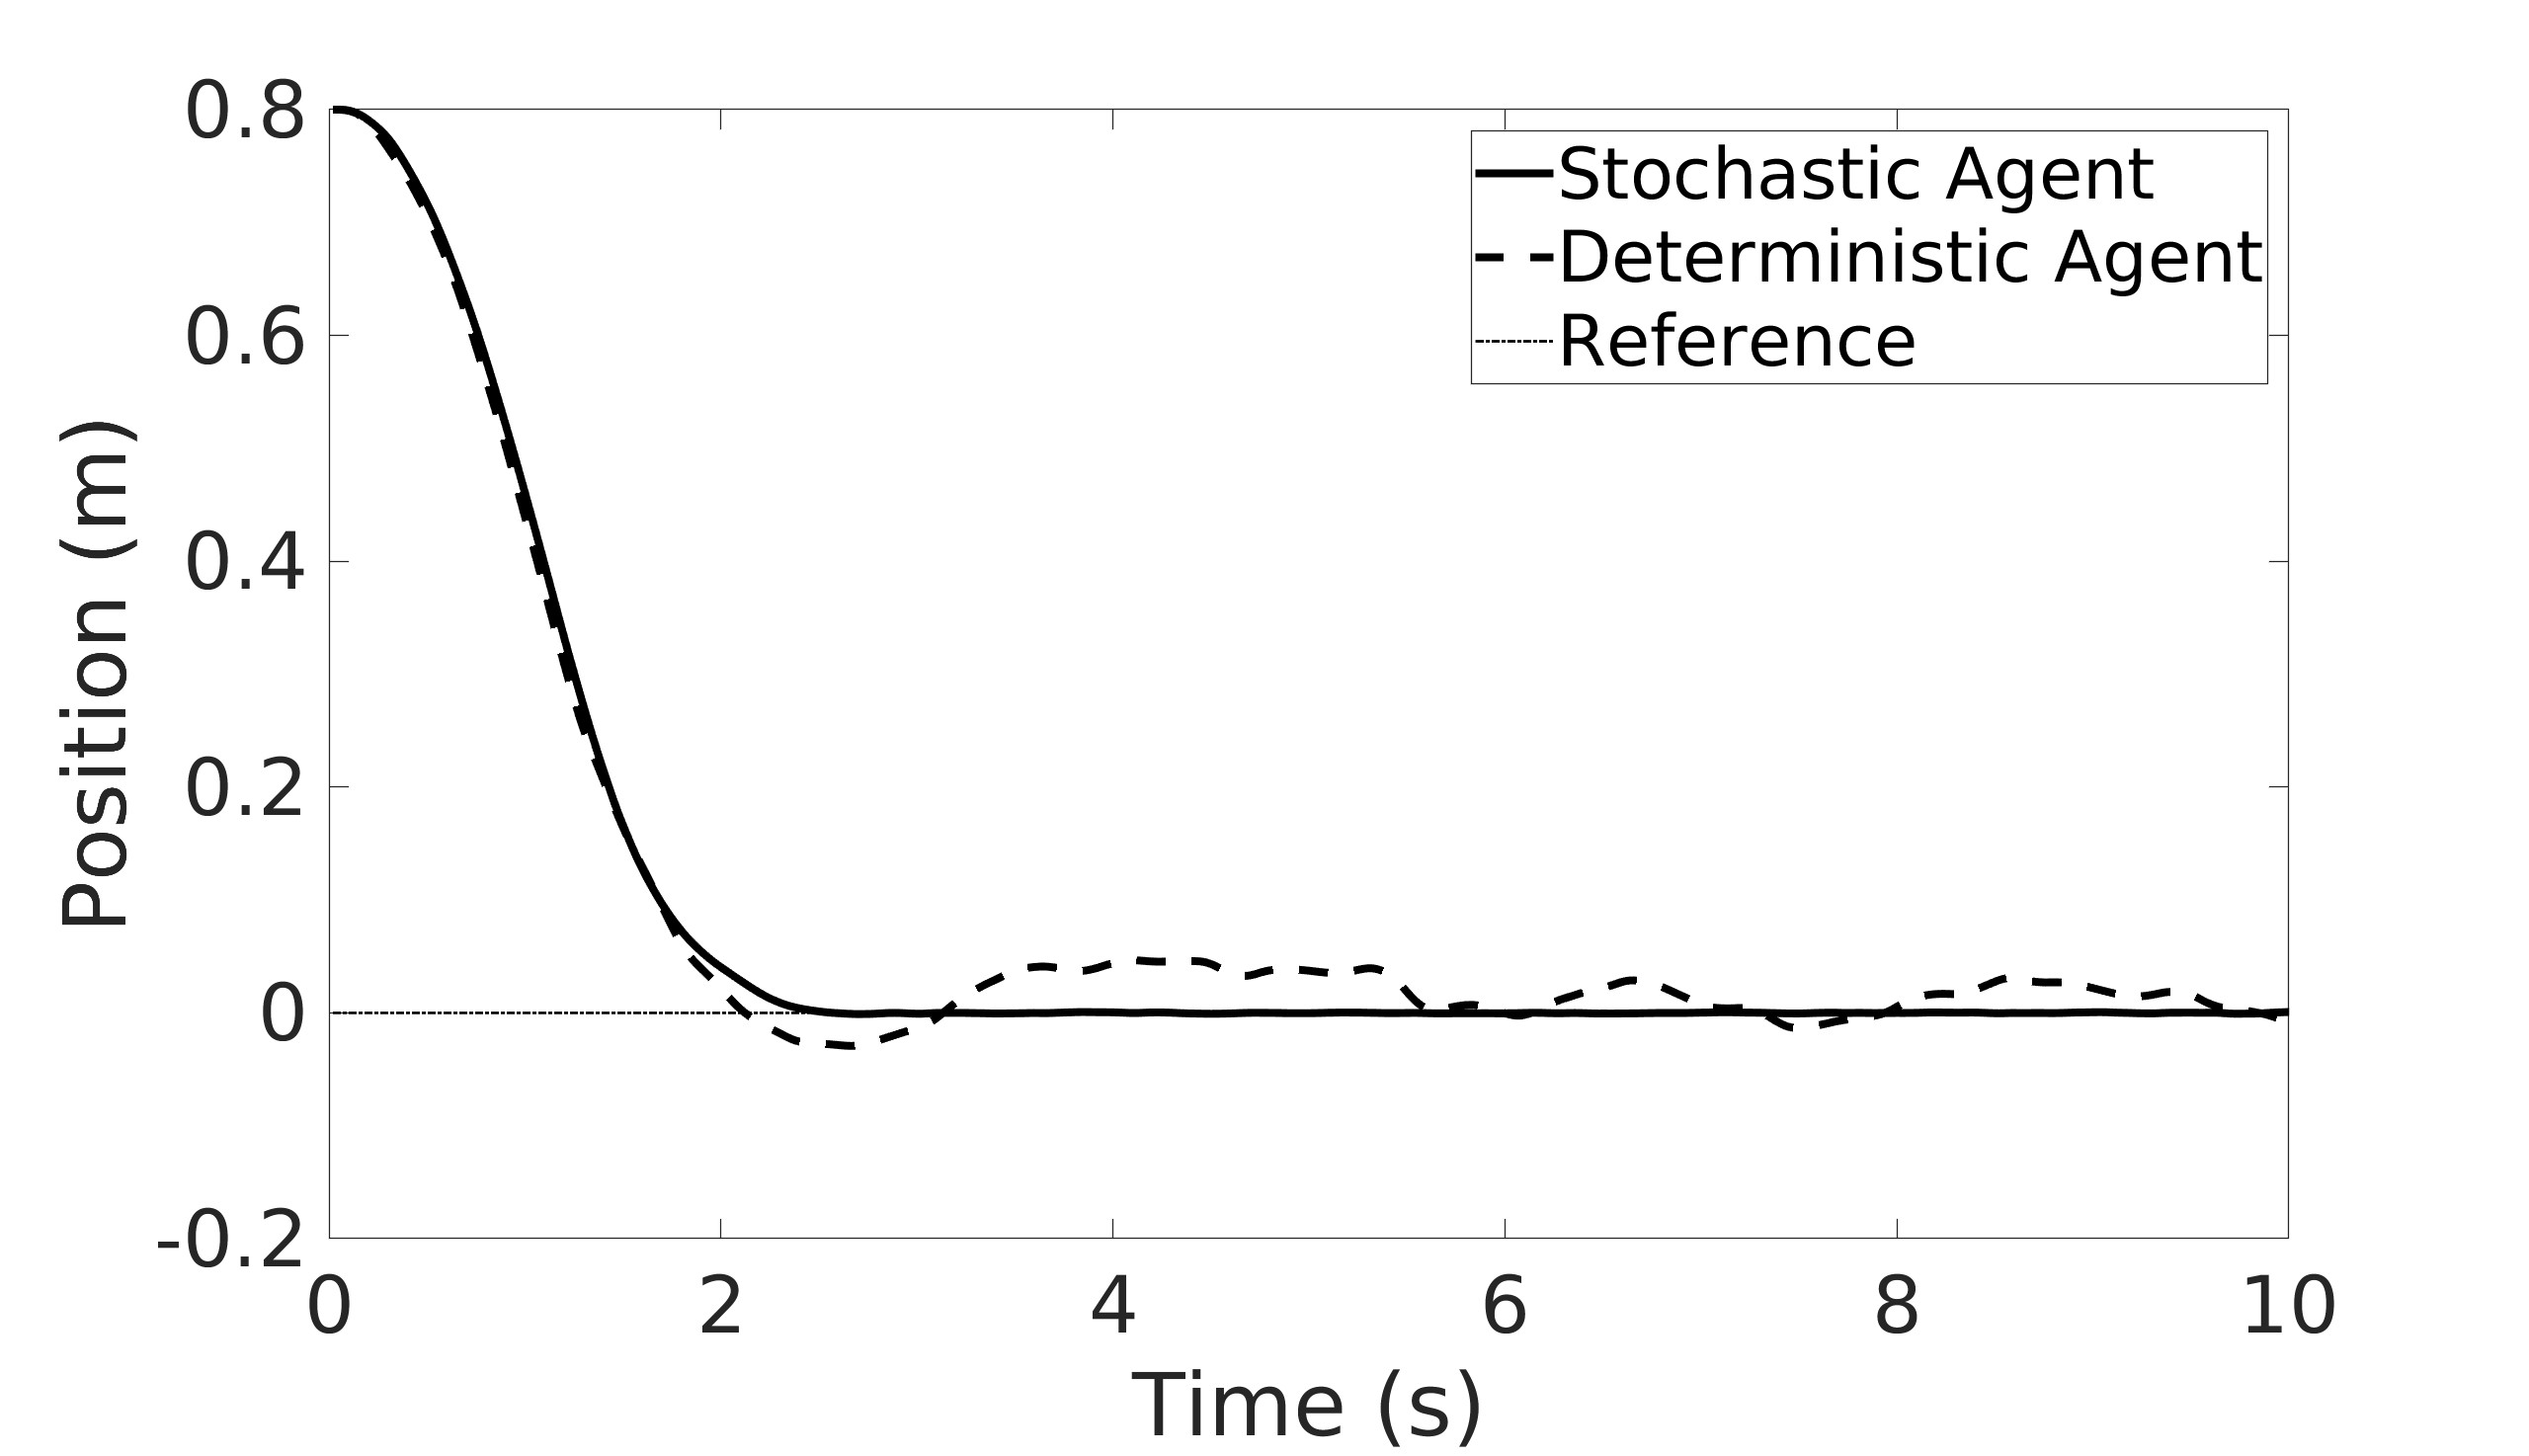
\includegraphics[width=0.75\textwidth]{plots/y1.jpg}
            \caption{$y$-axis Response for an Initial Position of 0.8 for Deterministic and Stochastic Position Controllers}
            \label{y1}
    \end{figure}
    For the $z$-axis response, the stochastic training agent stabilized with zero steady-state, a 0.12m overshoot and a settling time of 2.5 seconds as shown in Fig. \ref{z1}. The deterministic training agent on the other hand failed to stabilize.
    \begin{figure}[H]
            \centering
            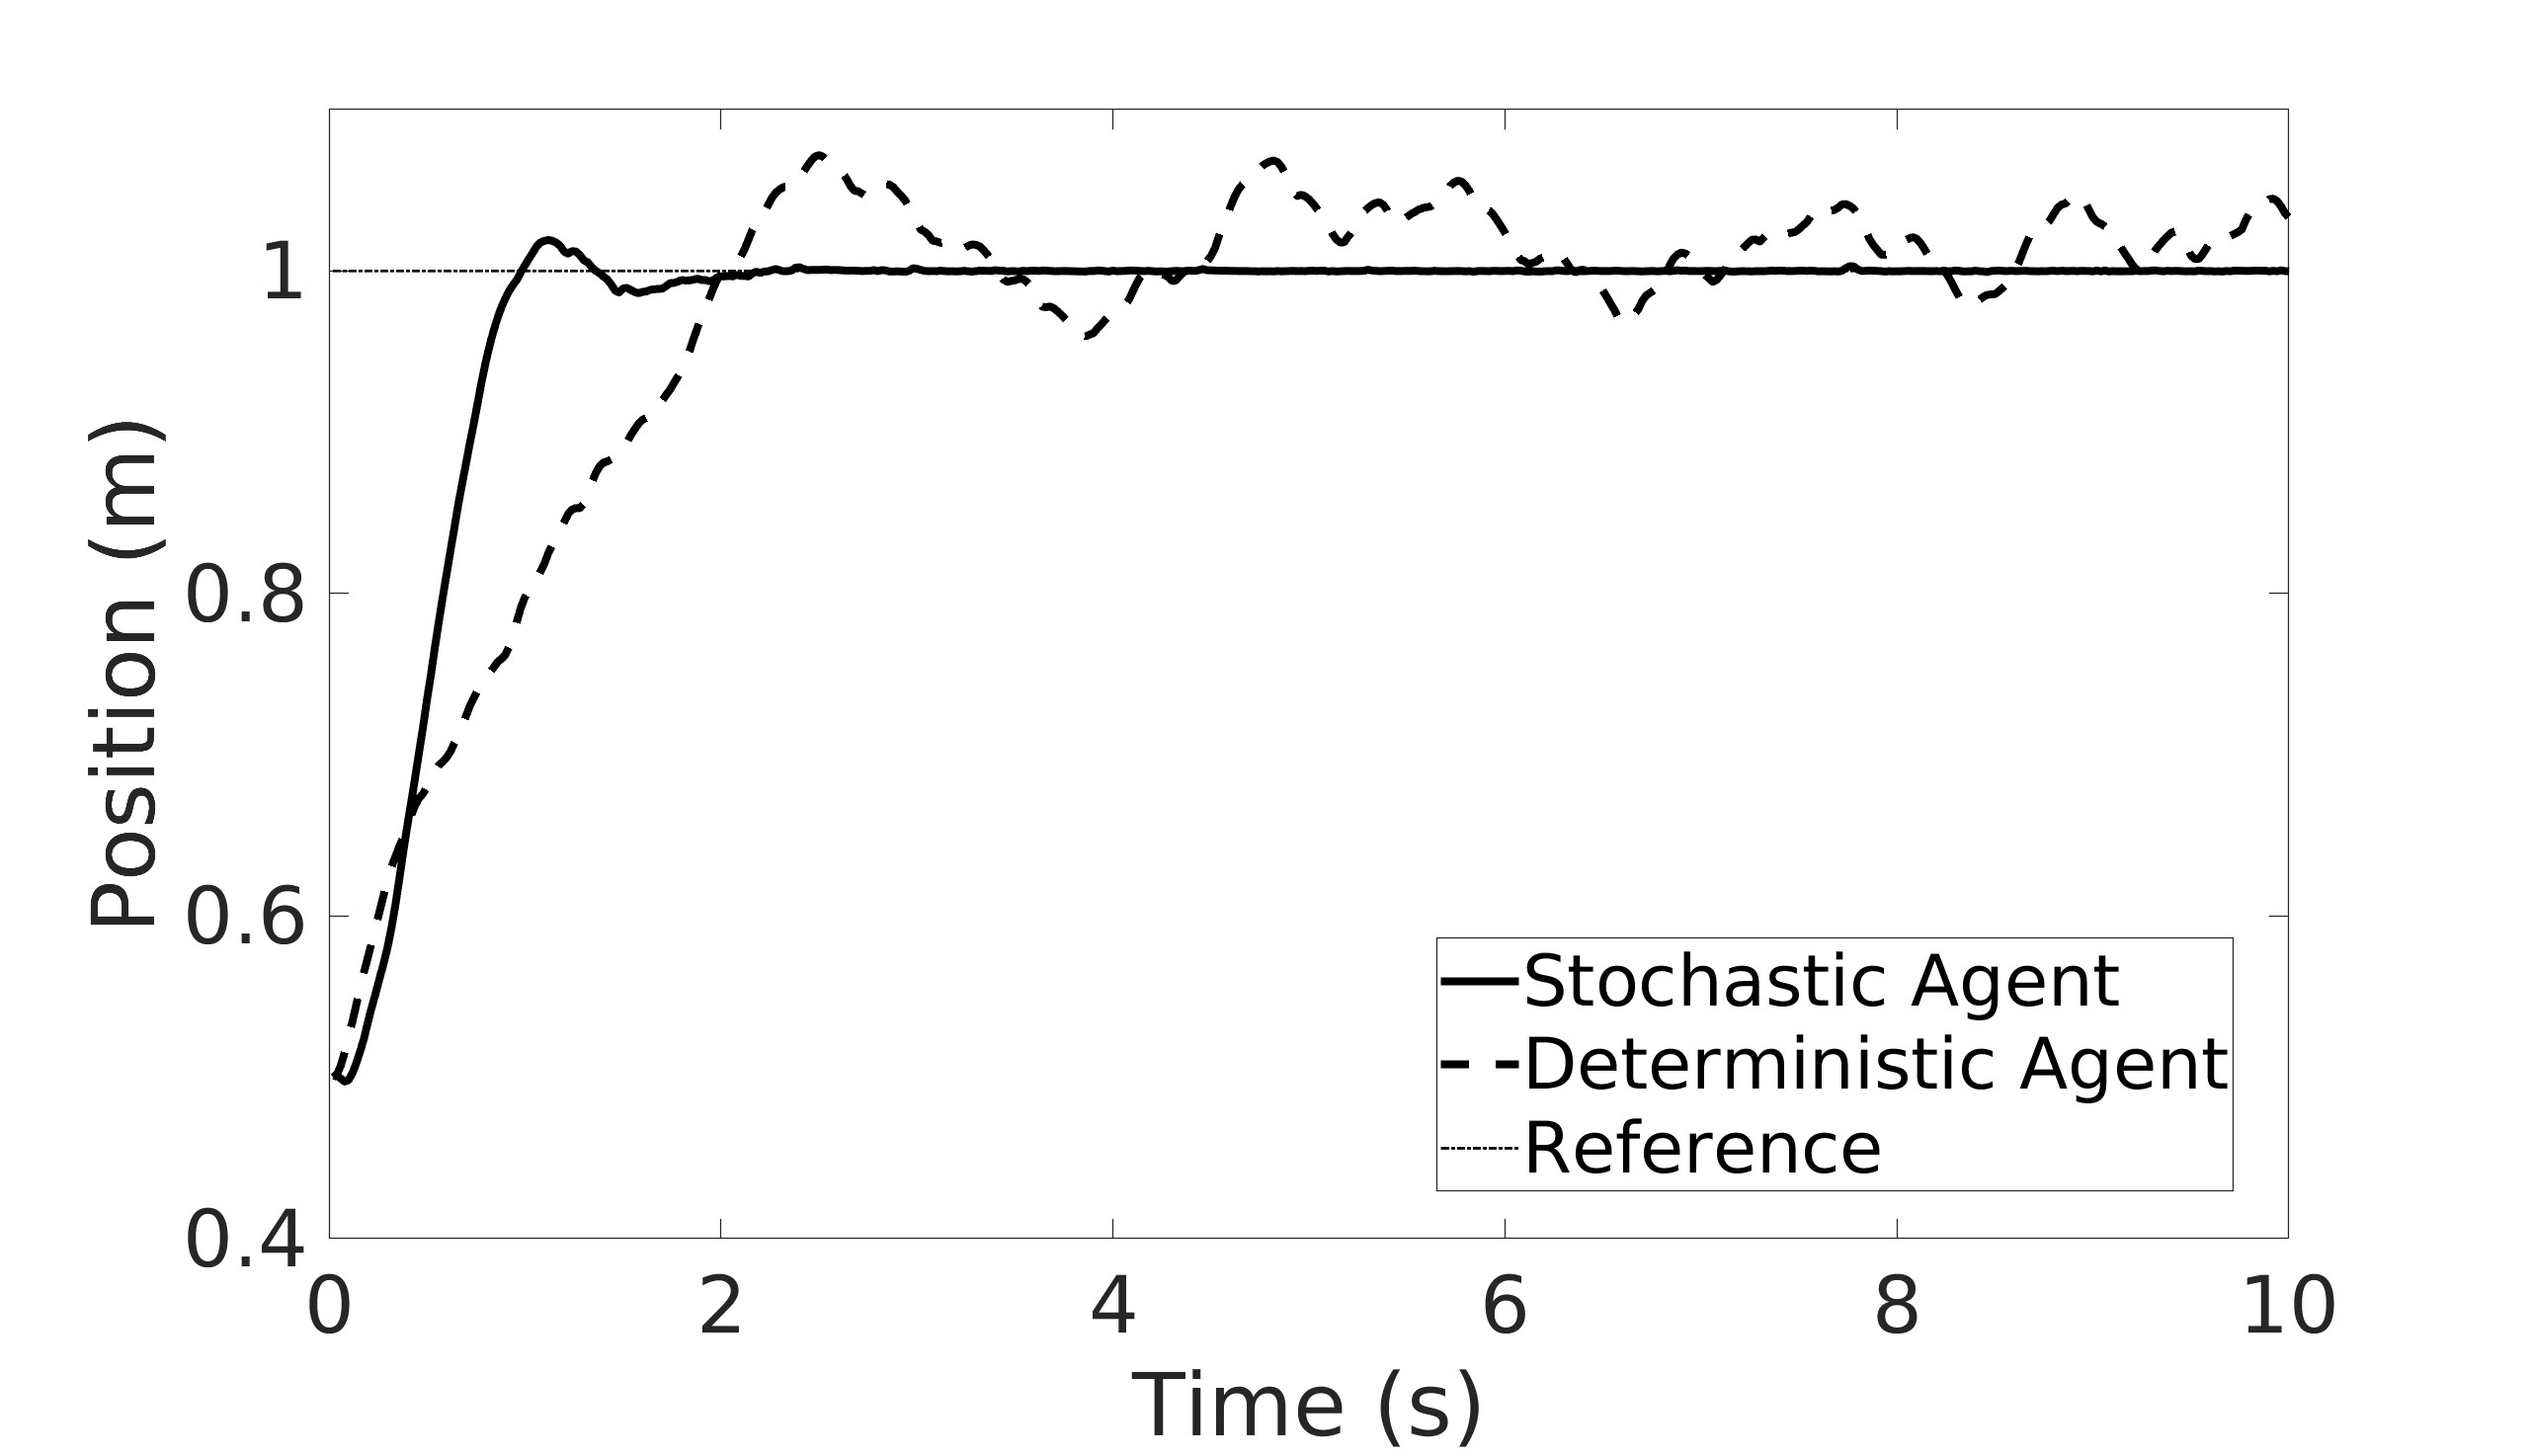
\includegraphics[width=0.75\textwidth]{plots/z1.jpg}
            \caption{$z$-axis Response for an Initial Position of 0.5 for Deterministic and Stochastic Position Controllers}
            \label{z1}
    \end{figure}
    \clearpage
    The advantages of stochastic algorithms become apparent in tasks requiring extensive exploration, such as the position controller task presented in this section. The position controller task requires a great deal of exploration because the agent does not receive immediate feedback on its actions. Instead, actions are sent to the PID attitude controller, which then computes the commands for the quadcopter. Theoretically, the critics evaluate the PID's actions rather than the agent's direct actions. This indirect feedback loop requires extensive exploration.\\

    This is further proven in Fig. \ref{X2}, Fig. \ref{y2} and Fig. \ref{z2}. These figures show the responses of the stochastic and deterministic training agents for the $x$-axis, $y$-axis and $z$-axis respectively when starting from an initial position of [-1.5, 1.5, 1.5]. This position is the most extreme position of the state space the agent was trained on.\\
    
    For the $x$-axis response, the stochastic training agent stabilized with zero steady-state, zero overshoot and a settling time of 2.5 seconds. The deterministic training agent on the other hand almost stabilized with a steady-state error of 0.07m and a settling time of 4.5 seconds.
    \begin{figure}[H]
            \centering
            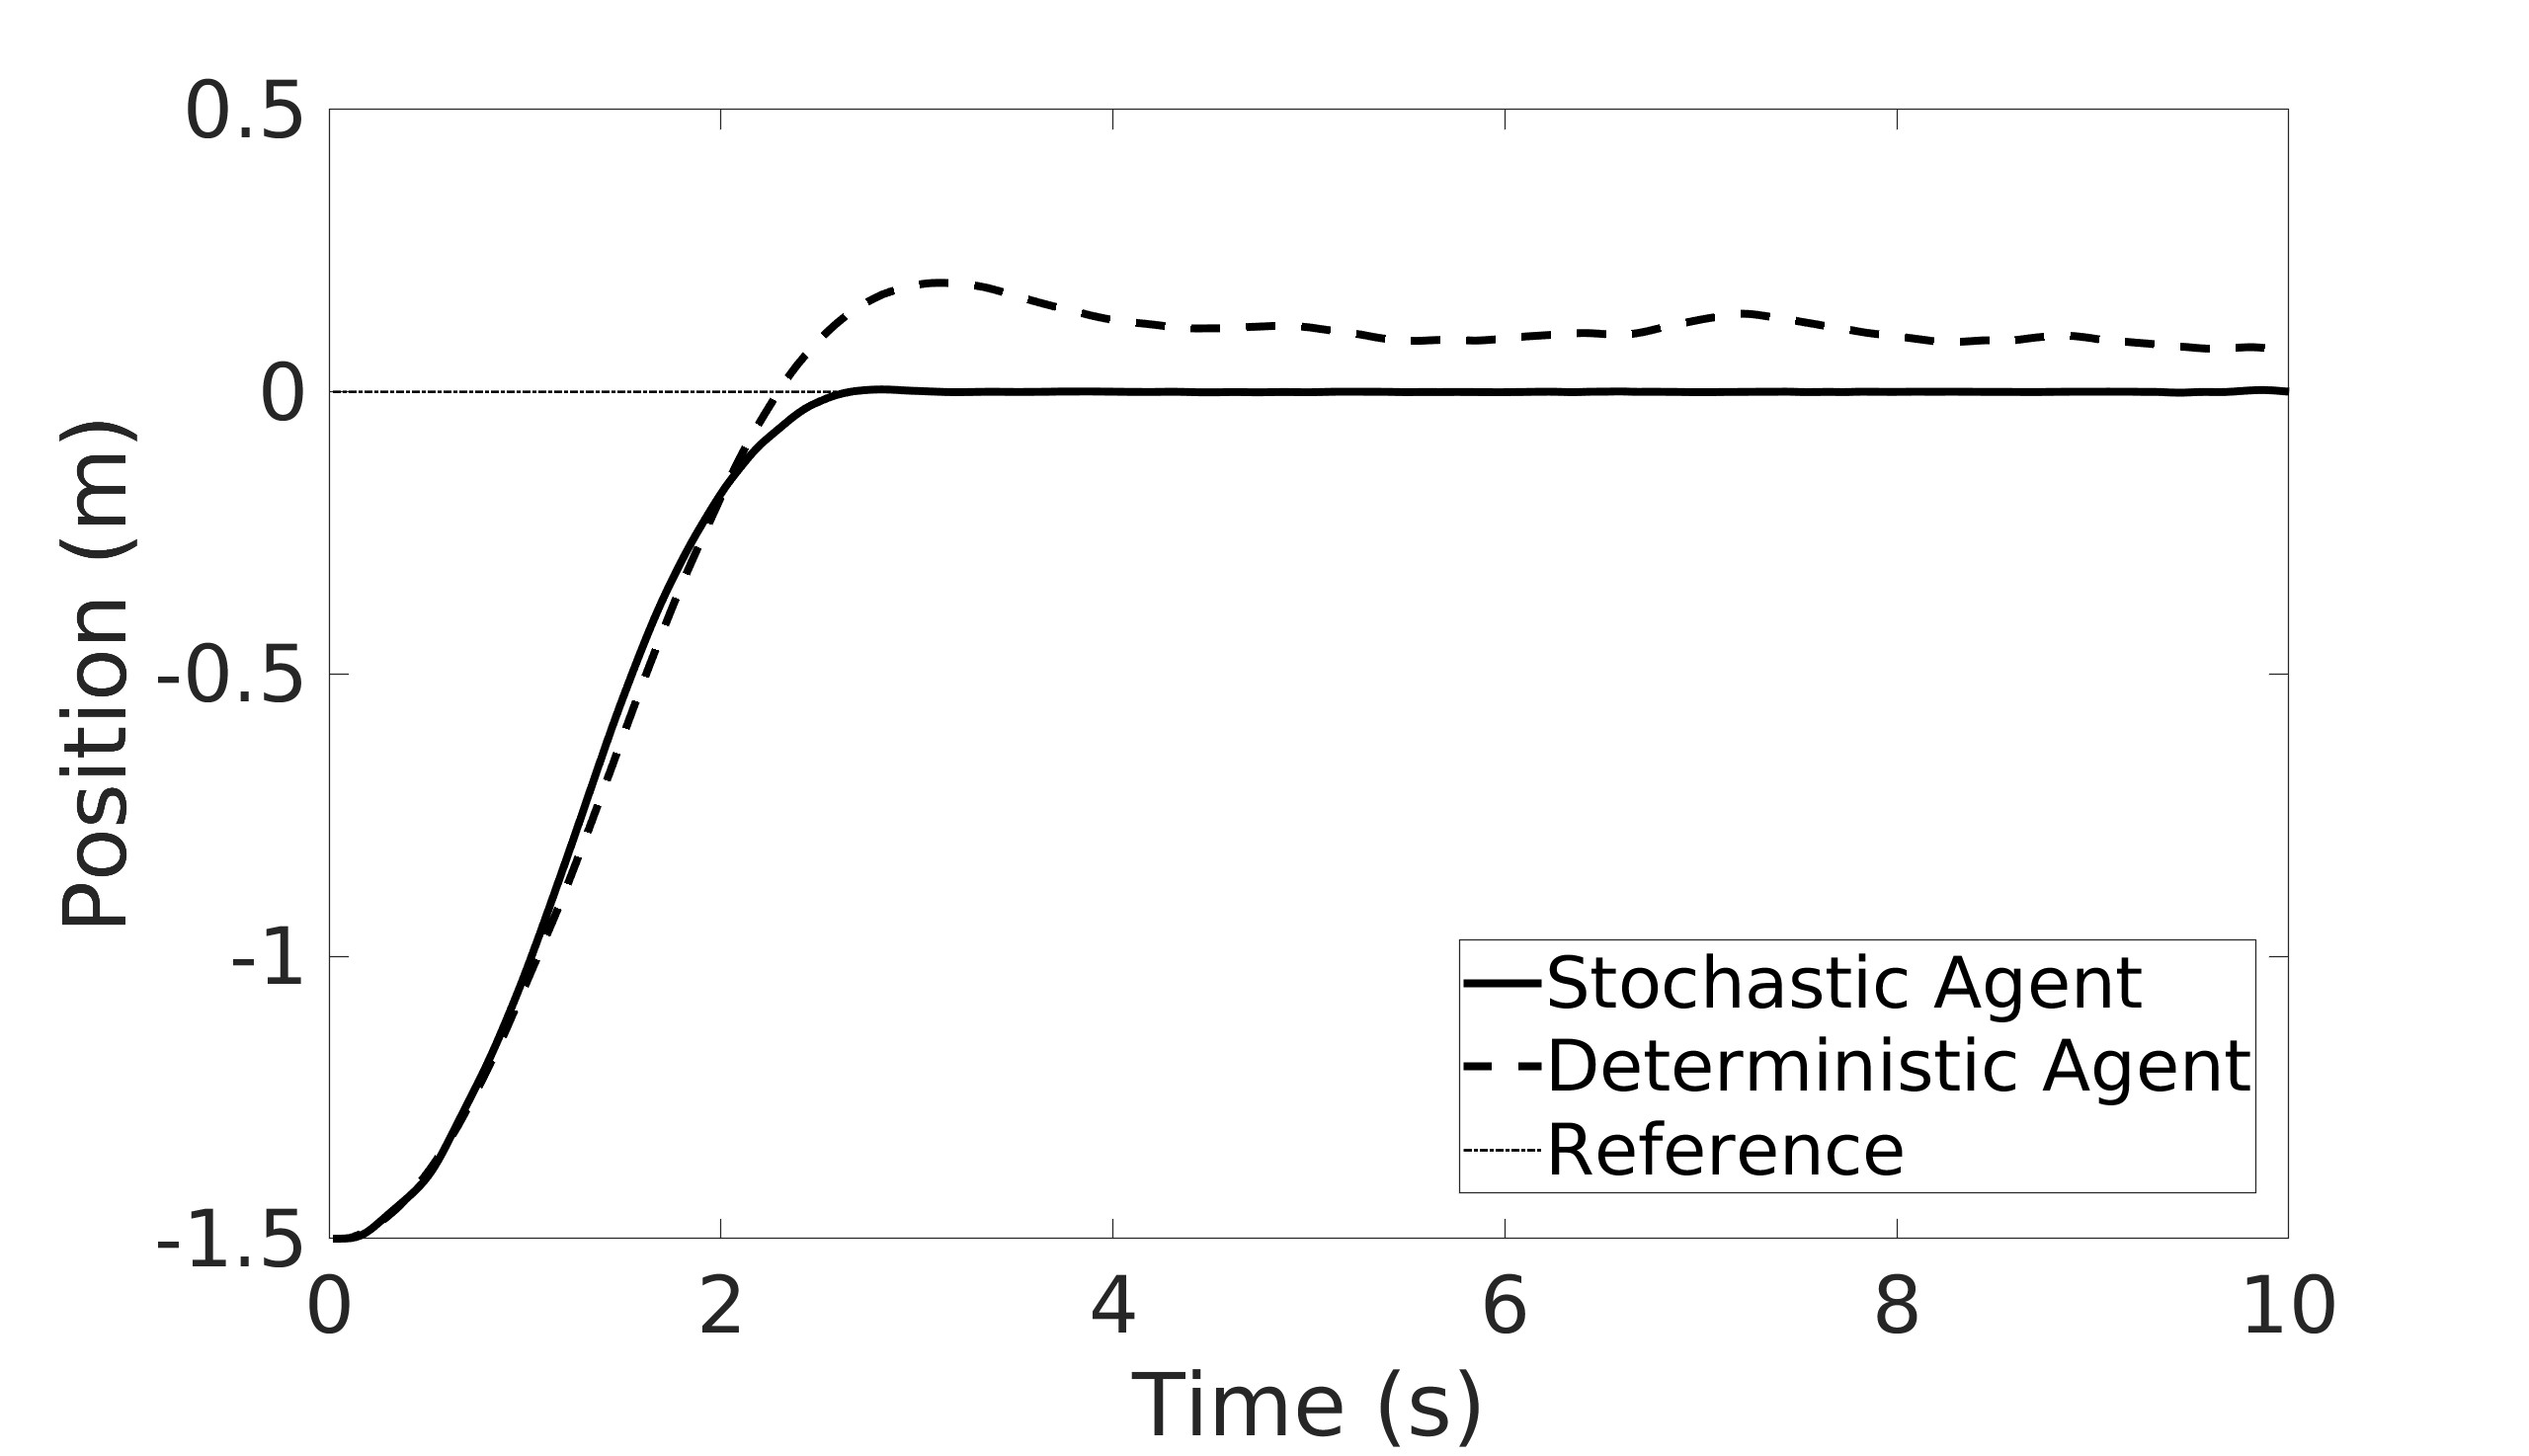
\includegraphics[width=0.75\textwidth]{plots/x2.jpg}
            \caption{$x$-axis Response for an Initial Position of -1.5 for Deterministic and Stochastic Position Controllers}
            \label{X2}
    \end{figure}\clearpage
    For the $y$-axis response, the stochastic training agent stabilized with zero steady-state, zero overshoot and a settling time of 2.5 seconds. The deterministic training agent on the other hand stabilized with a settling time of 8.5 seconds as shown in Fig. \ref{y2}.
    \begin{figure}[H]
            \centering
            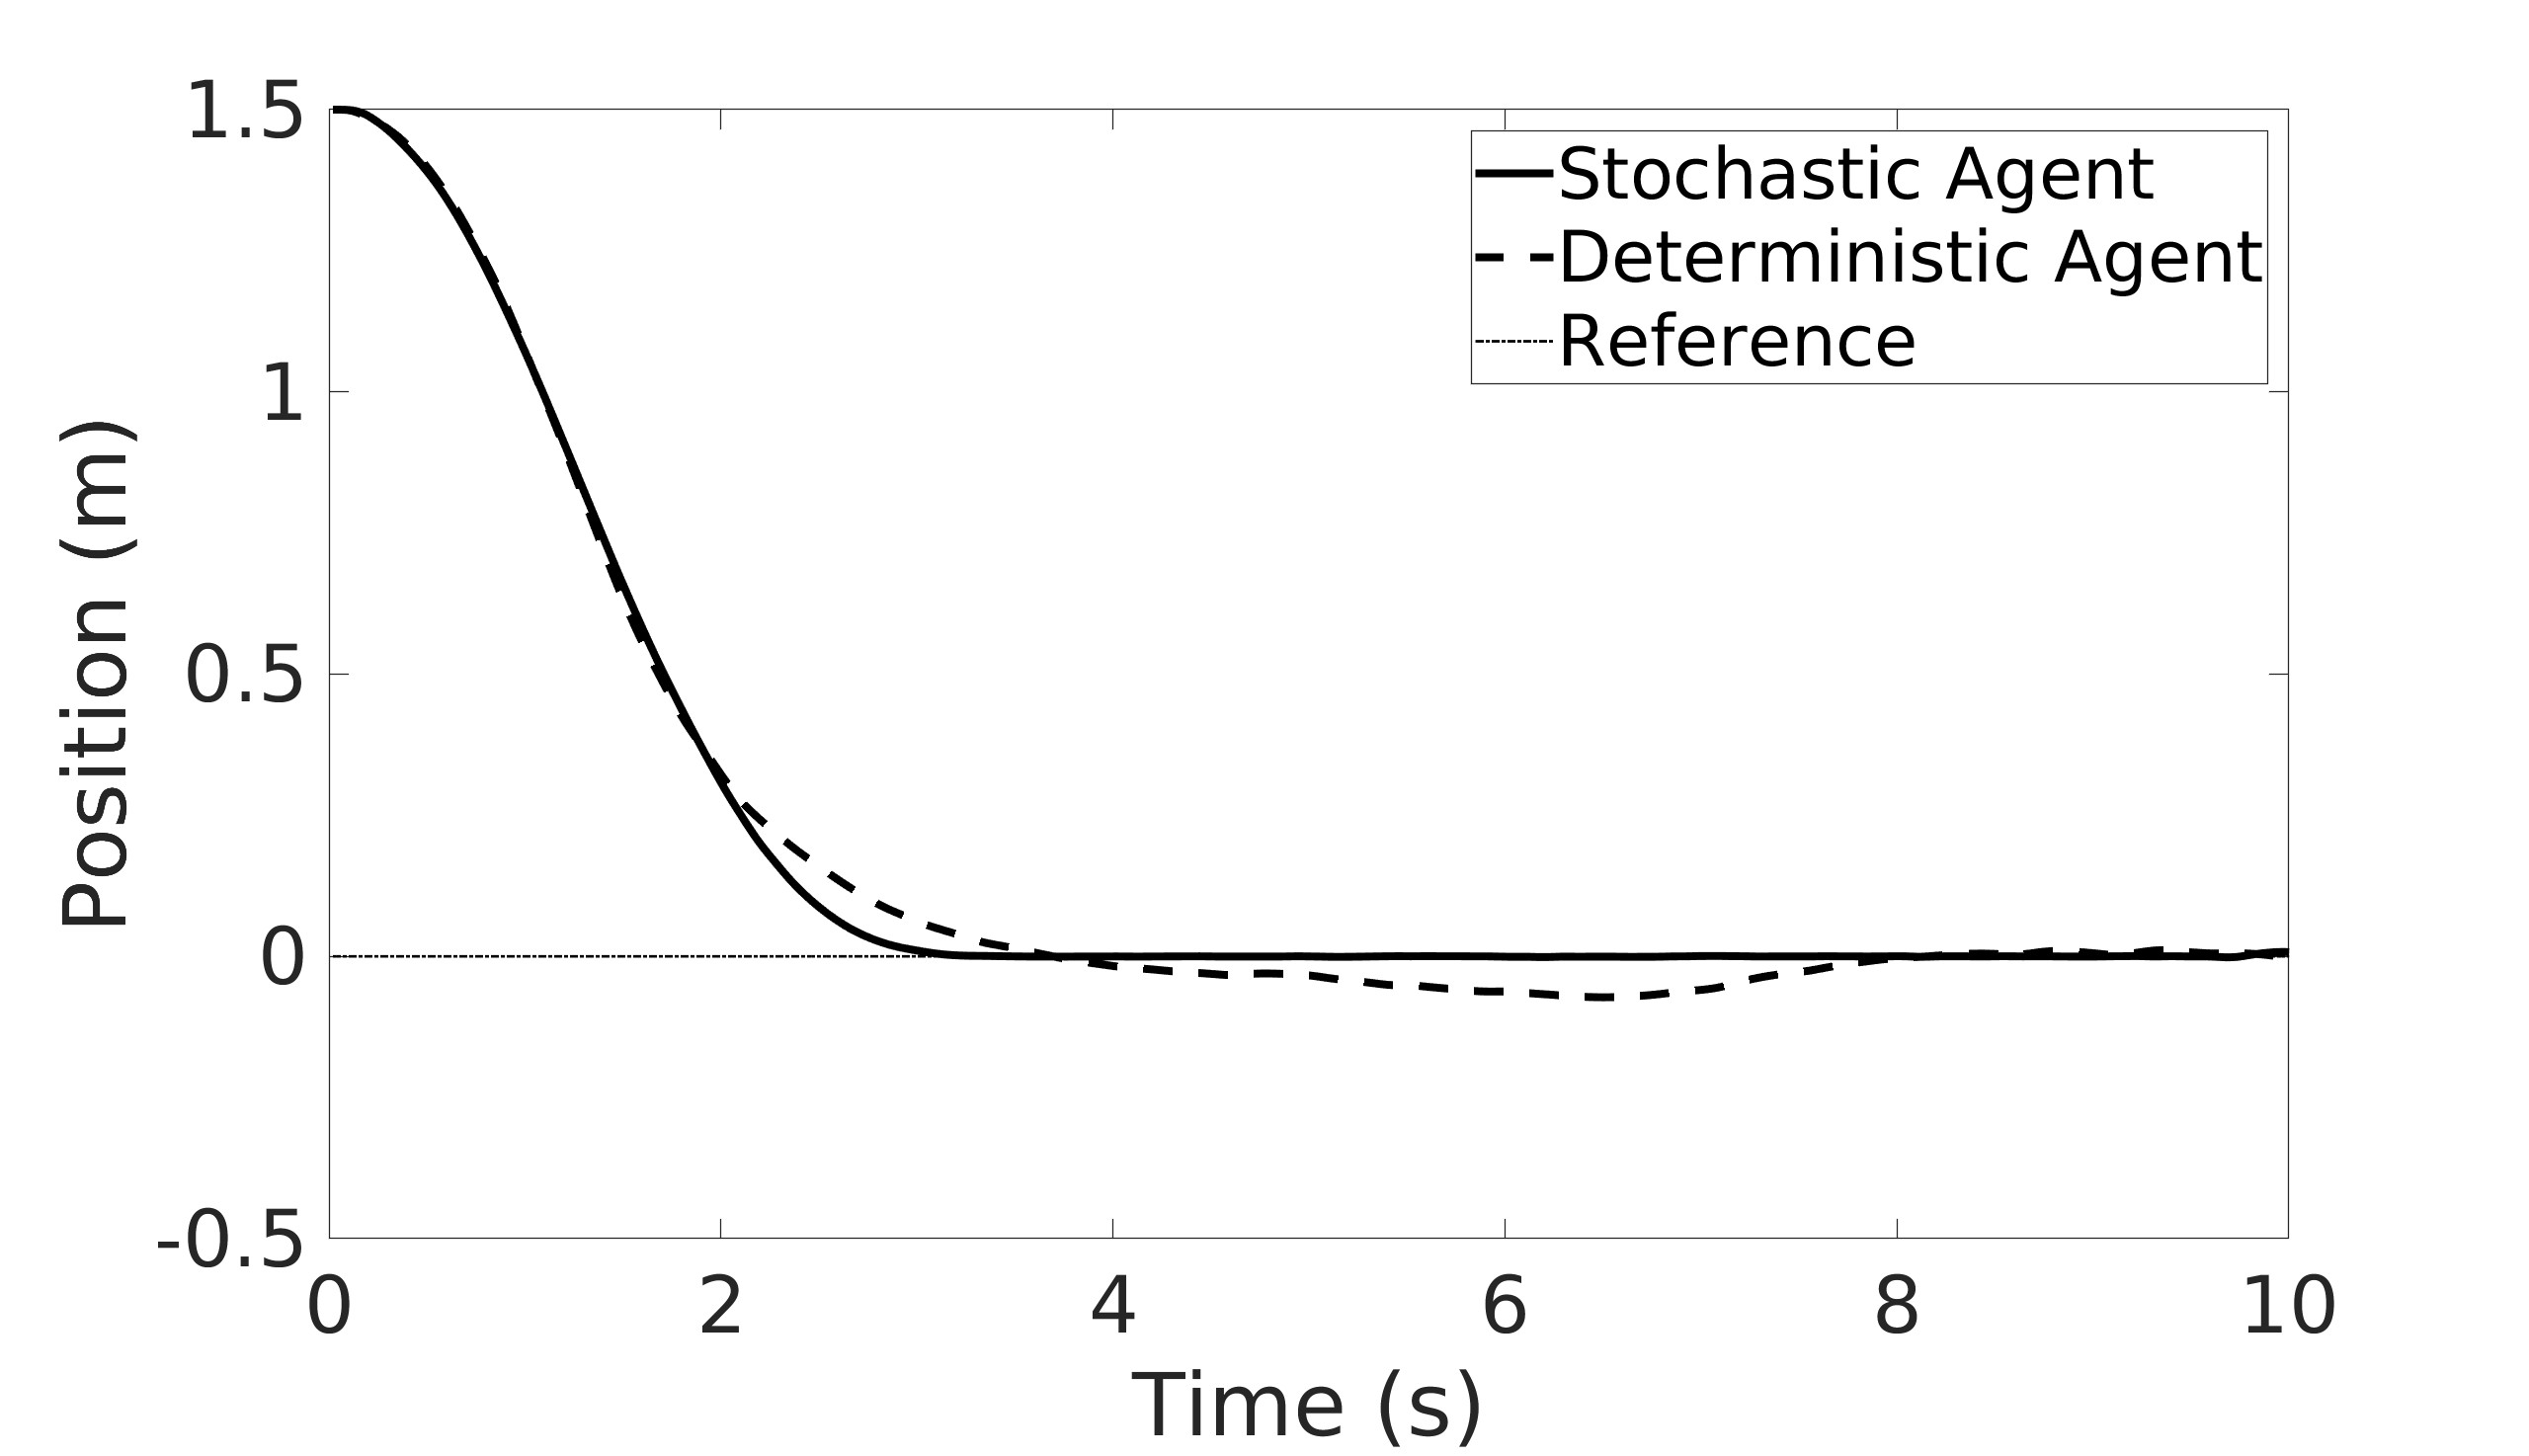
\includegraphics[width=0.75\textwidth]{plots/y2.jpg}
            \caption{$y$-axis Response for an Initial Position of 1.5 for Deterministic and Stochastic Position Controllers}
            \label{y2}
    \end{figure}
    For the $z$-axis response in Fig. \ref{z2}, the stochastic training agent stabilized with zero steady-state, a 0.02m overshoot and a settling time of 2.5 seconds. The deterministic training agent on the other hand failed to stabilize.
    \begin{figure}[H]
            \centering
            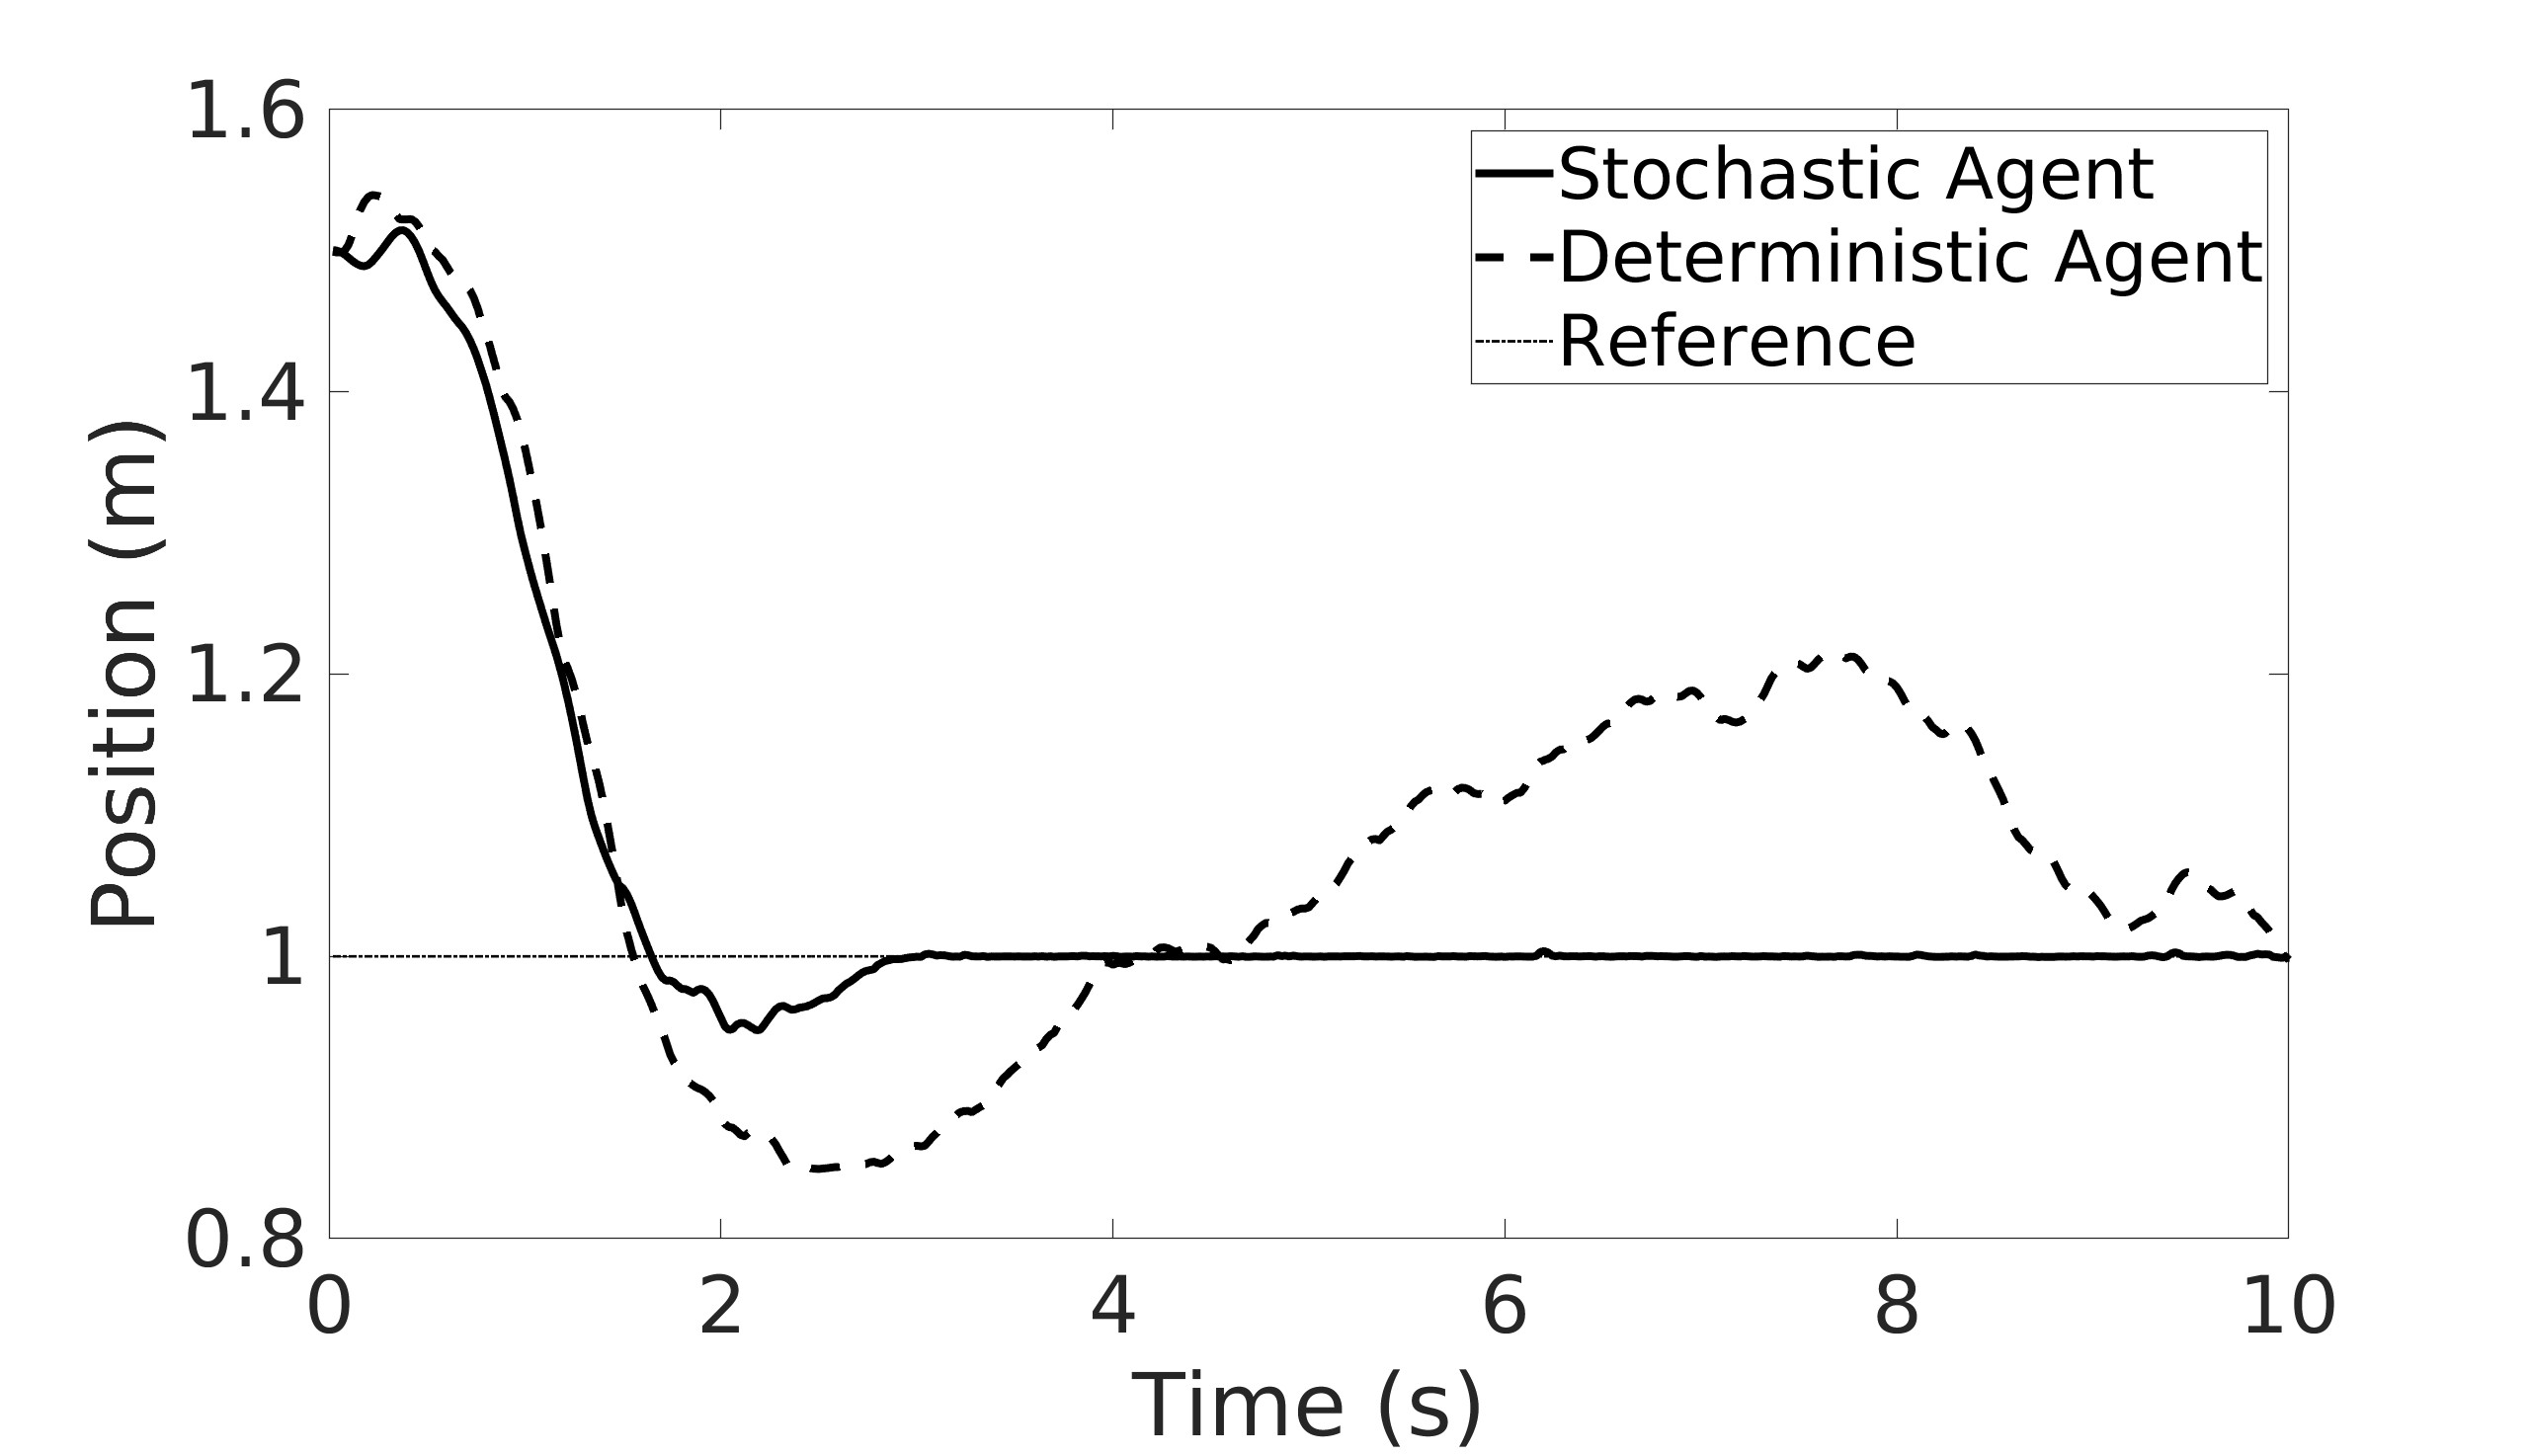
\includegraphics[width=0.75\textwidth]{plots/z2.jpg}
            \caption{$z$-axis Response for an Initial Position of 1.5 for Deterministic and Stochastic Position Controllers}
            \label{z2}
    \end{figure}\clearpage
    %######################################################################
    \section{Trajectory Tracking Training}
    The objective of this training was for the agent to reach and stabilize the quadcopter starting from a random position however, this time reaching a random position each episode. Since the deterministic algorithm's stabilizing results were not sufficient, the stochastic algorithm was only used in the rest of the thesis. Fig. \ref{trrew} shows the mean reward obtained by the stochastic agent. The agent was trained for a total of 1,362,500 steps with the maximum reward reached at the 918,500 step with a value of 65,570.8 as shown.
      \begin{figure}[H]
            \centering
            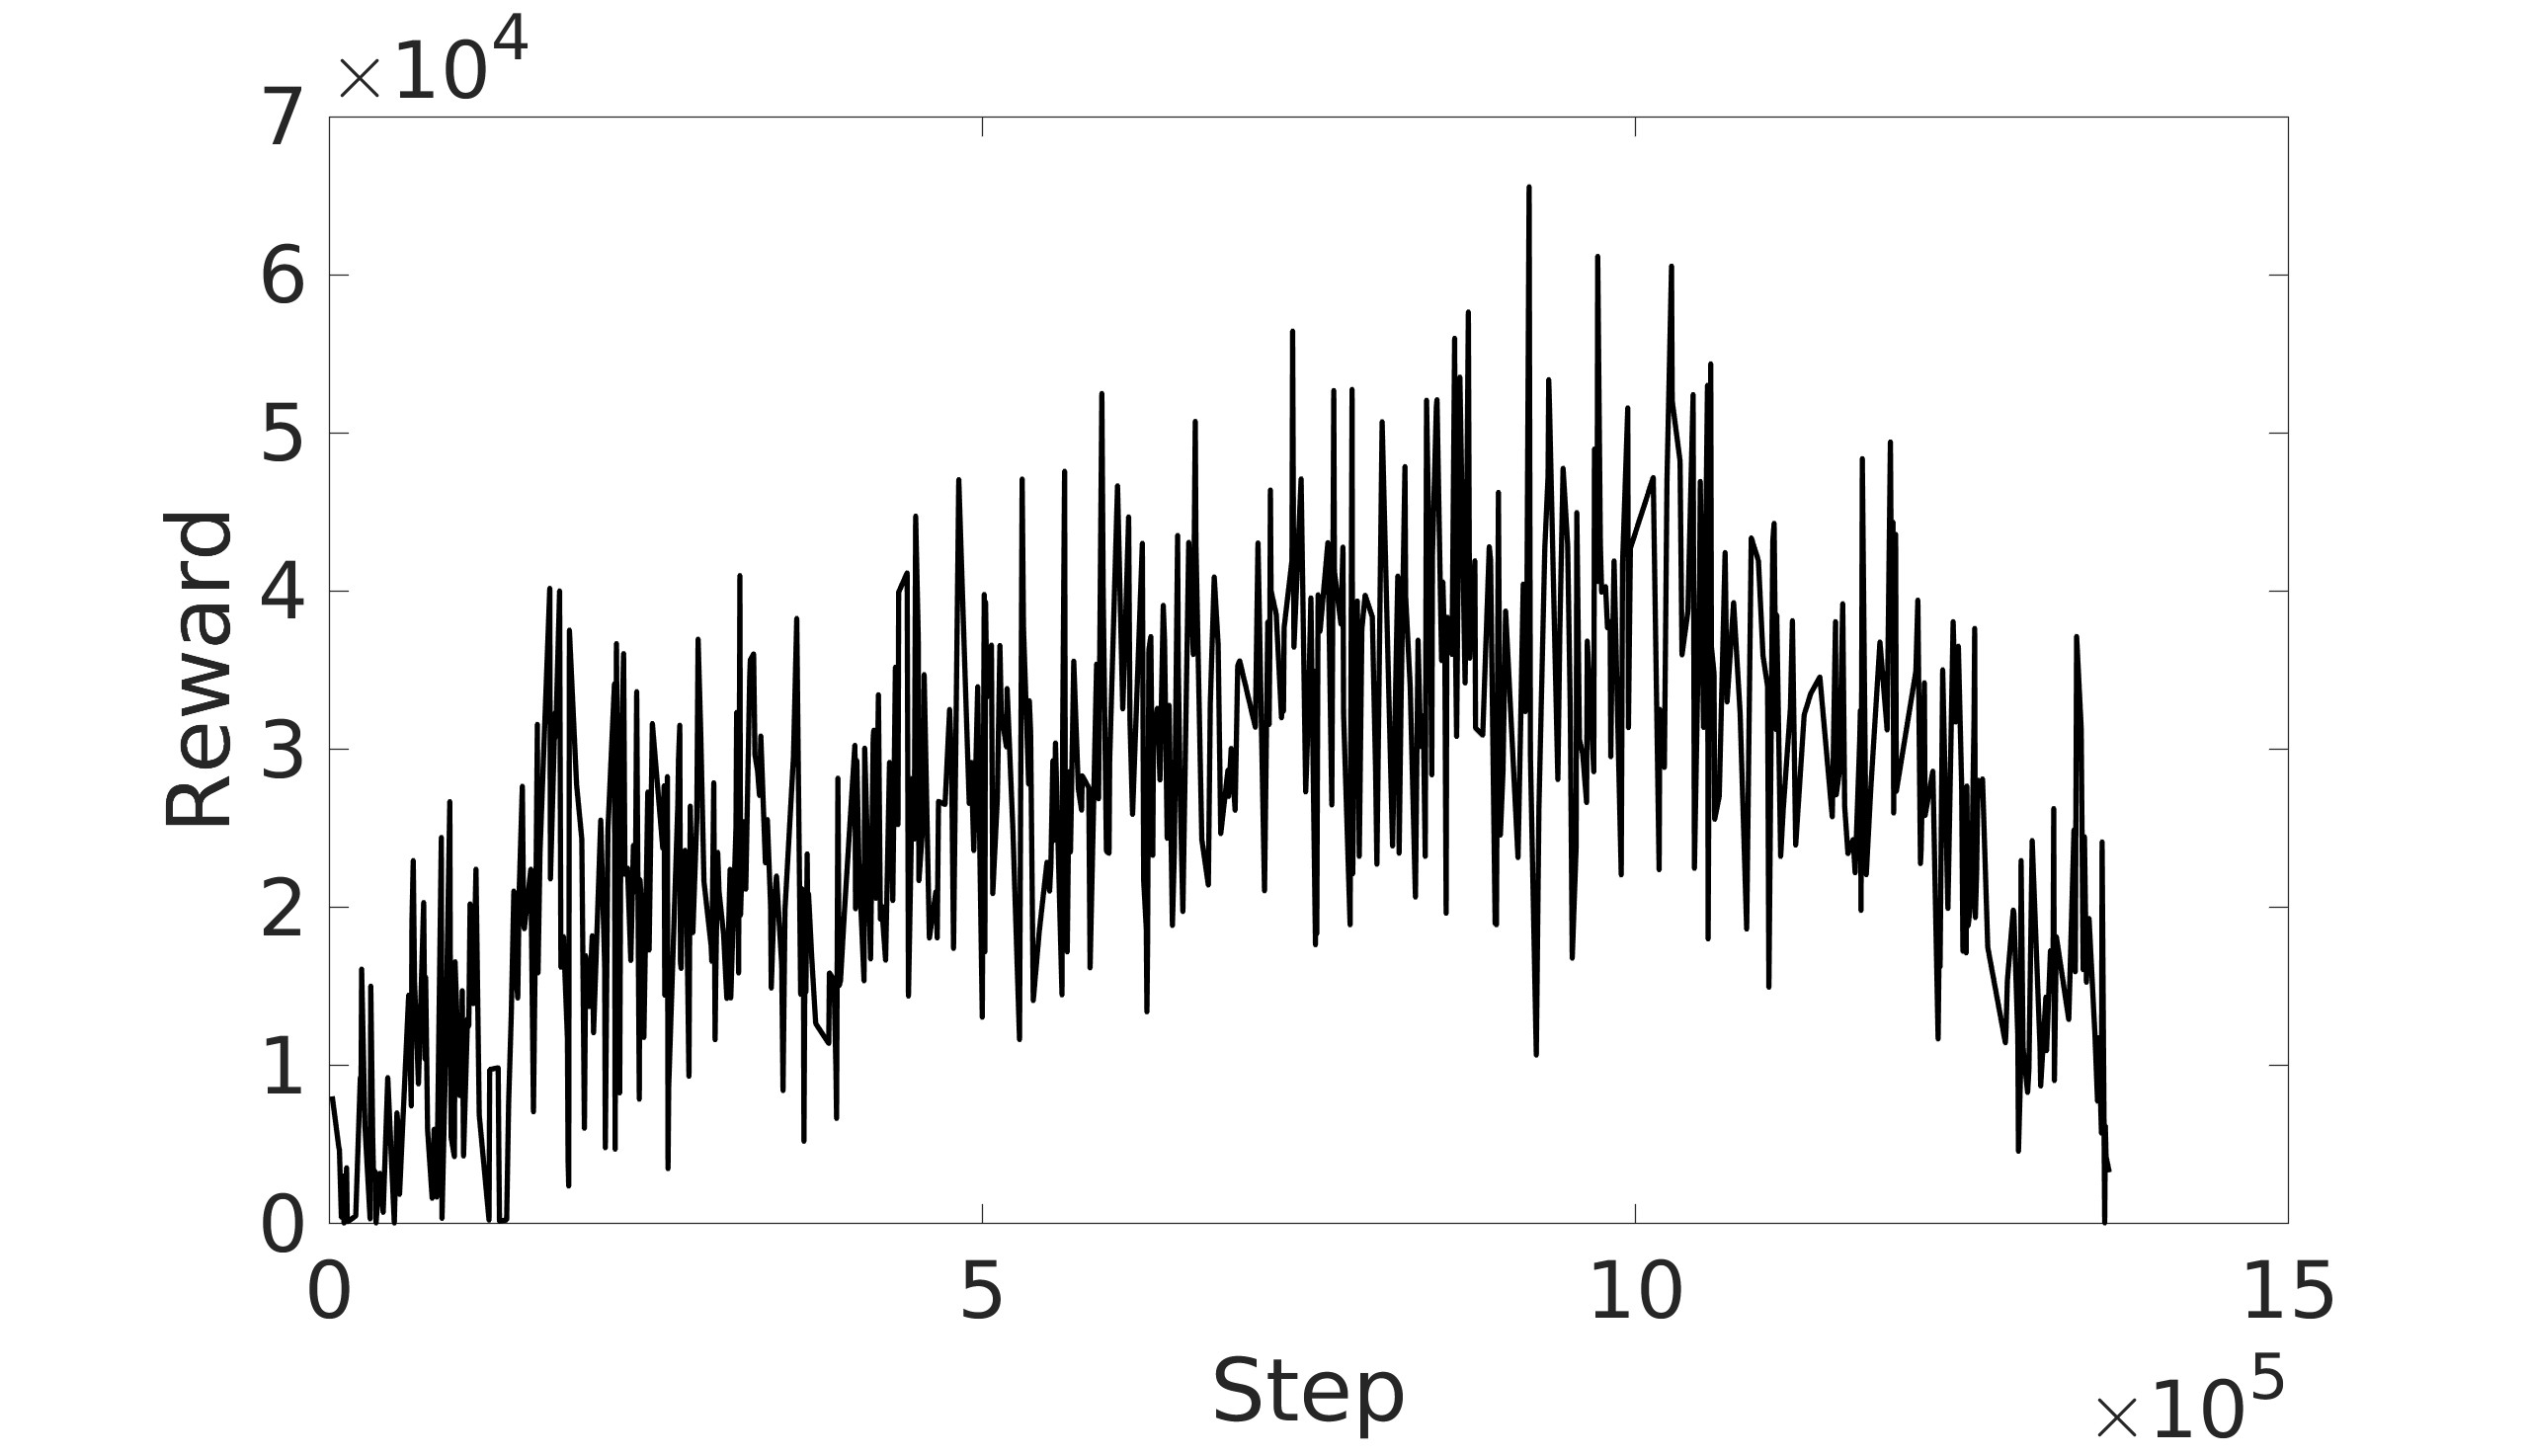
\includegraphics[width=0.75\textwidth]{plots/track_rew.jpg}
            \caption{Mean Reward for the Trajectory Tracking Training of Stochastic Position Controller}
            \label{trrew}
    \end{figure}
     Fig. \ref{trackpos1} shows the stochastic agent response when starting from an initial position of [-0.35, -1.1, 1.75] and reaching a target at [0.5, -0.5, 0.5]. The agent stabilized with zero steady-state error in all three axes. The agent had zero overshoot across all axes with a settling time of 3 seconds.
    \begin{figure}[H]
            \centering
            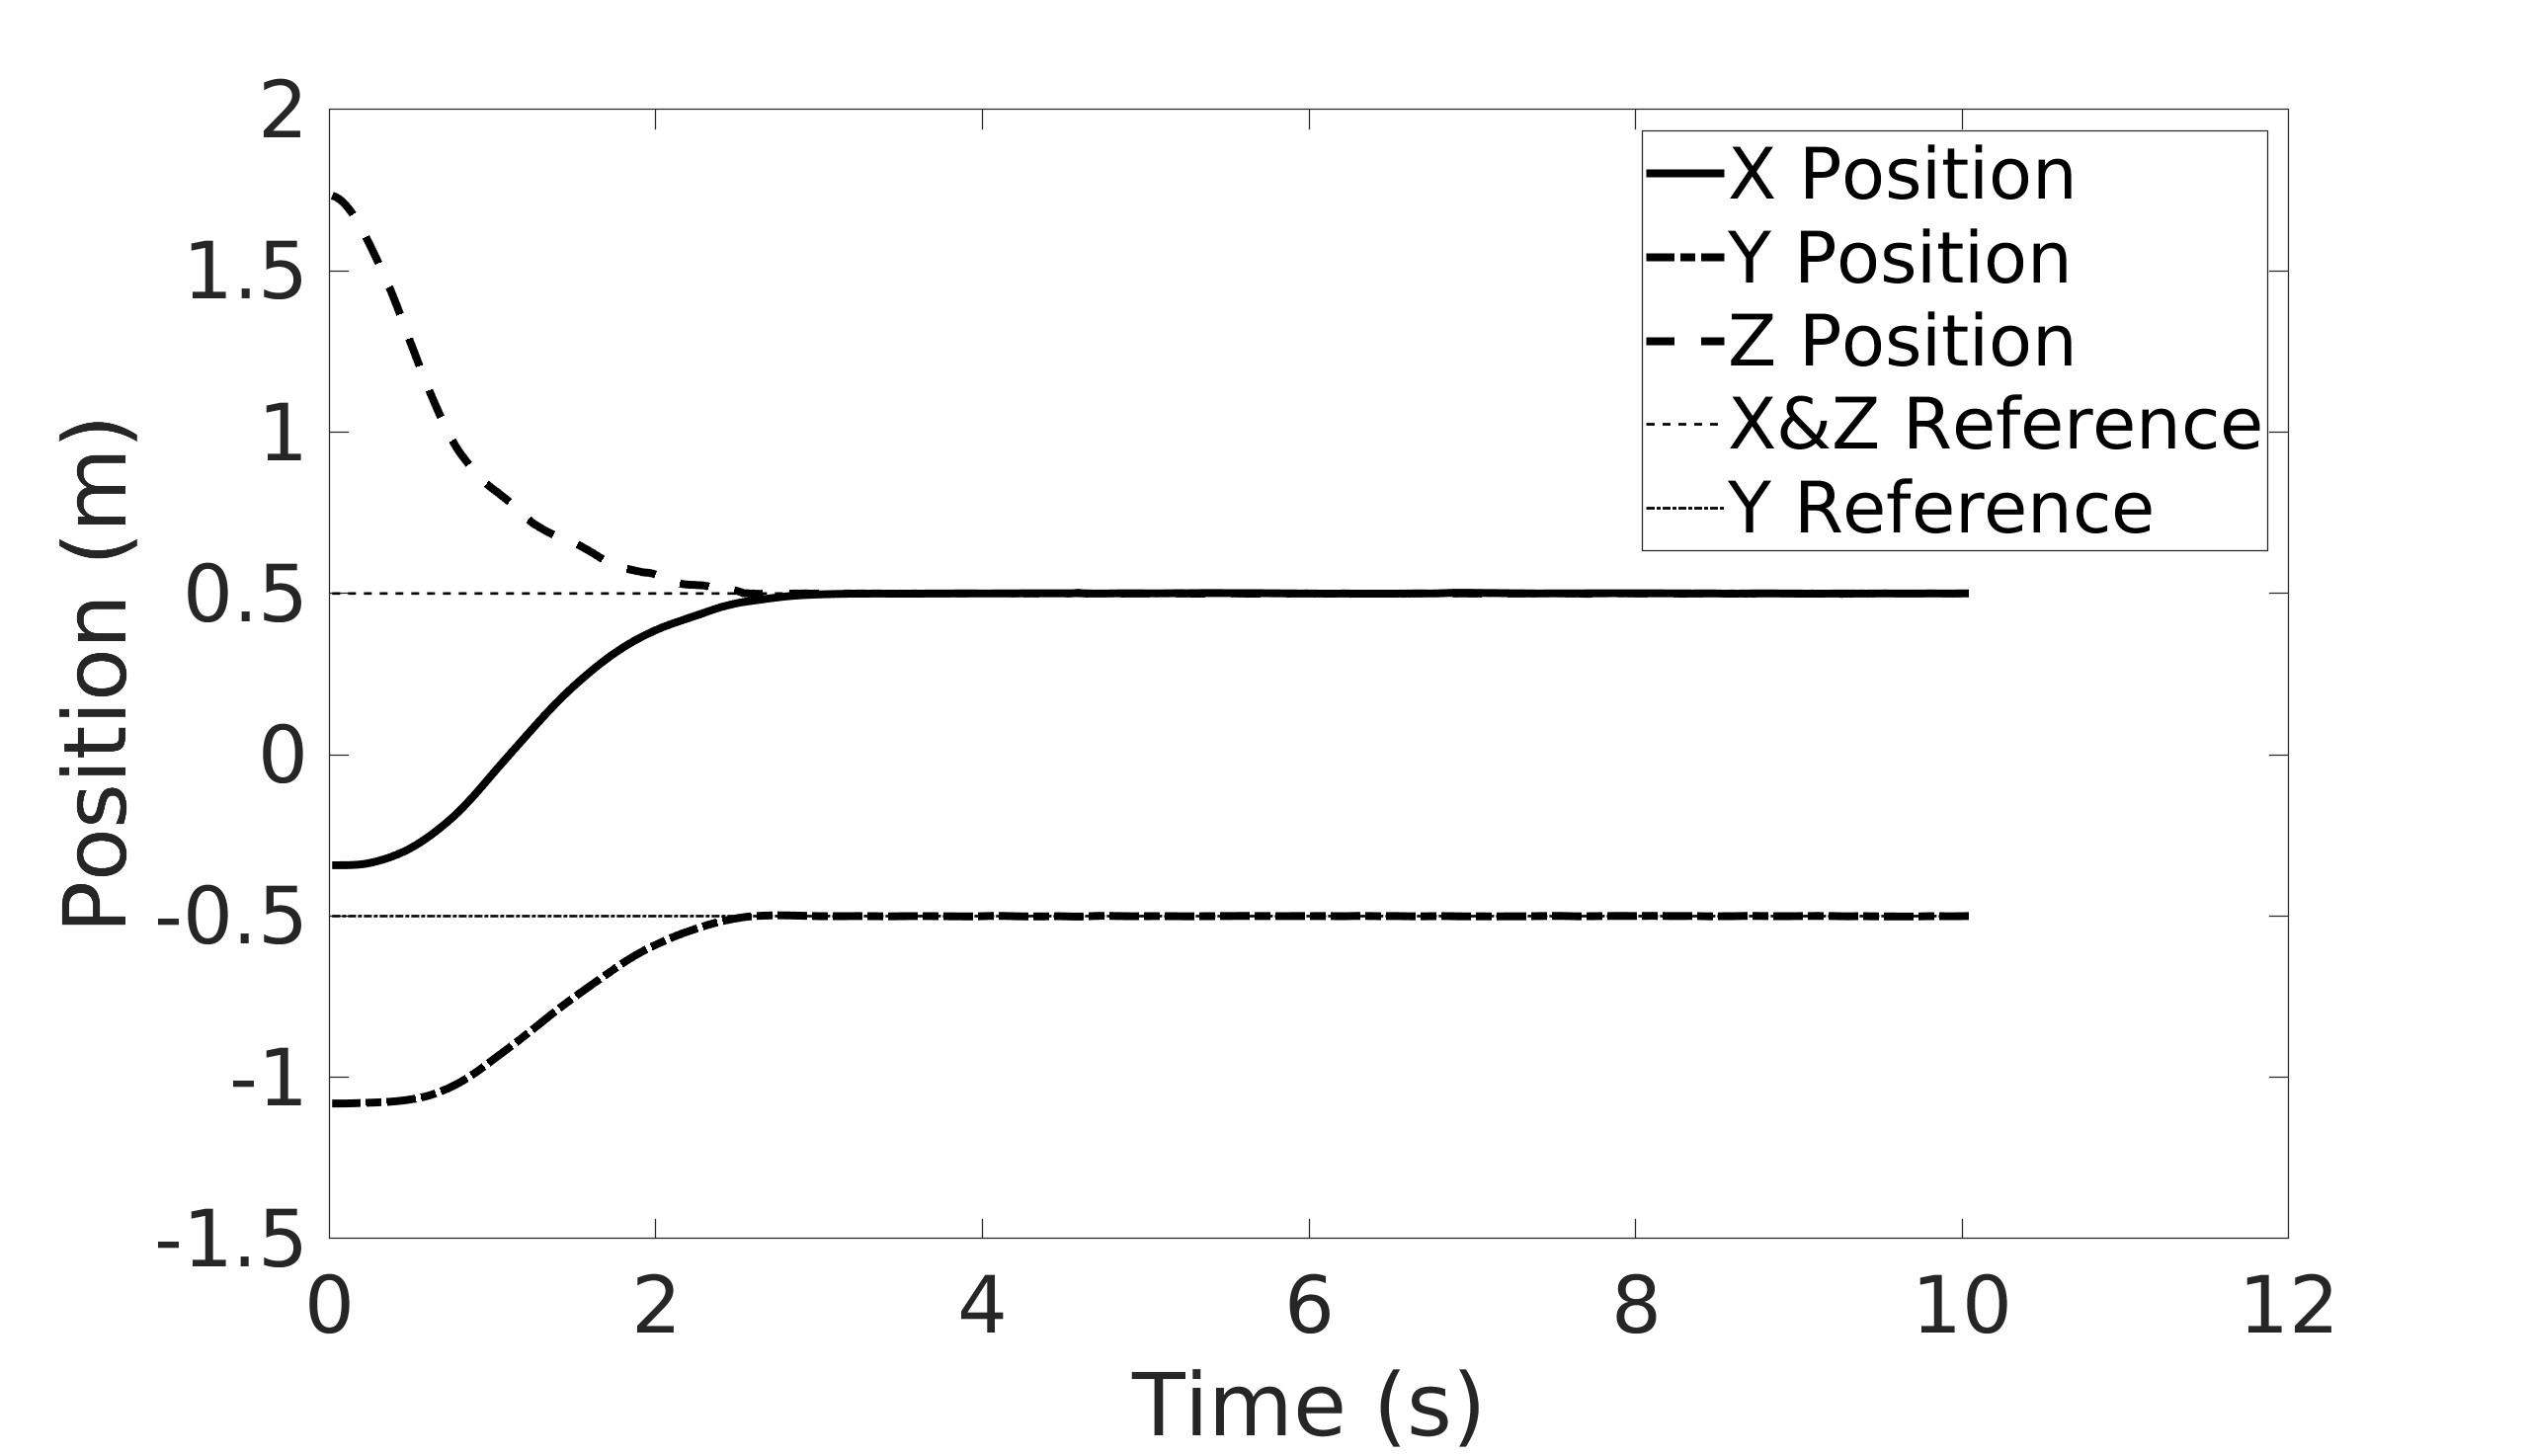
\includegraphics[width=0.75\textwidth]{plots/track1_pos.jpg}
            \caption{Stochastic Trajectory Tracking Agent Response for a Target Position of [0.5, -0.5, 0.5]}
            \label{trackpos1}
    \end{figure}
    Fig. \ref{trpos2} shows the SAC response when starting from another initial position of [-0.2, 1.2, 1.6] and reaching a target at [1.4, 1.8, 1.2]. The agent stabilized with zero steady-state error in all three axes. The agent had zero overshoot across all axes with a settling time of 3.5 seconds.
    \begin{figure}[H]
            \centering
            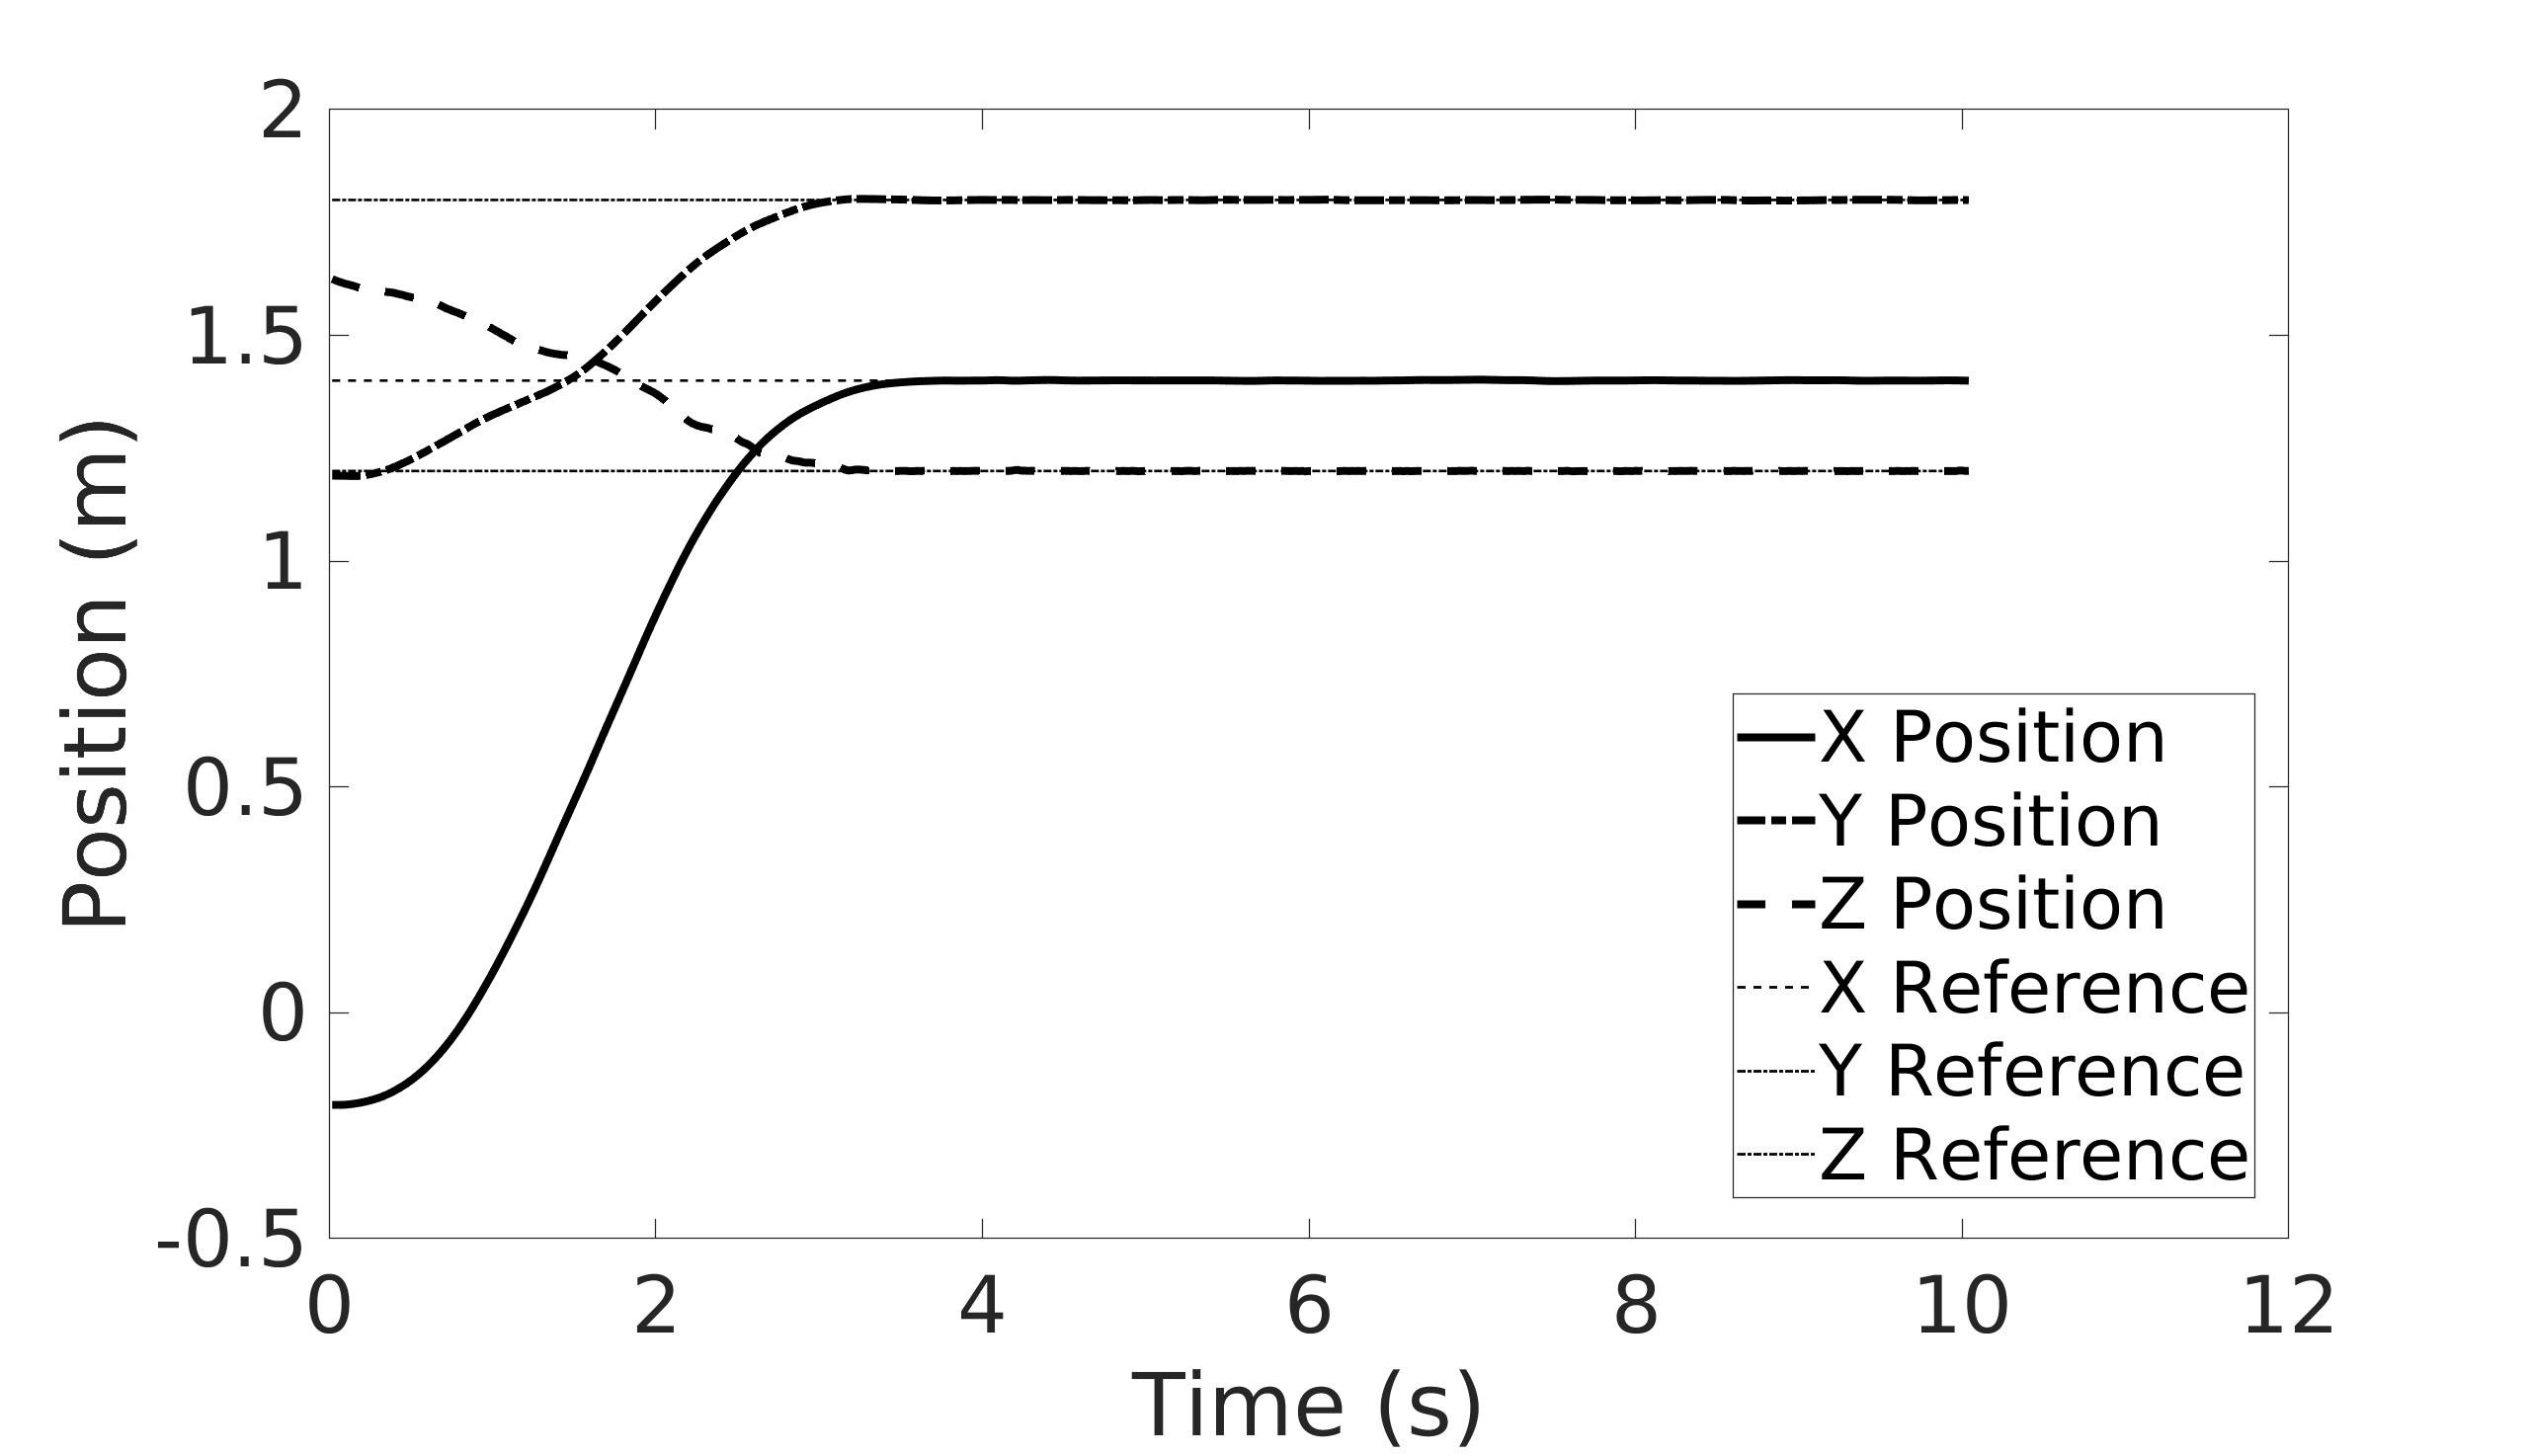
\includegraphics[width=0.75\textwidth]{plots/track2_pos.jpg}
            \caption{Stochastic Trajectory Tracking Agent Response for a Target Position of [1.4, 1.8, 1.2]}
            \label{trpos2}
    \end{figure}\clearpage
    %#######################################################################
    \section{Position Controller}
    The obtained agent was integrated as a position controller. After the trajectory tracking training, the agent was able to track any given trajectory without prior training. The trajectory tested was based on a parametric equation derived from the Lemniscate of Bernoulli shown in Eq. \ref{traj}.\\
    \begin{equation}
    x = \frac{0.5 cos(t)}{1 + sin^2(t)}\hspace{20pt} y = \frac{0.5 sin(t) cos(t)}{1 + sin^2(t)} \hspace{20pt} z = x + 1.5
        \label{traj}
    \end{equation}\\
    Fig. \ref{traj2} shows the successful tracking of the trajectory with a smooth path achieved by the stochastic position controller.
    \begin{figure}[H]
            \centering
            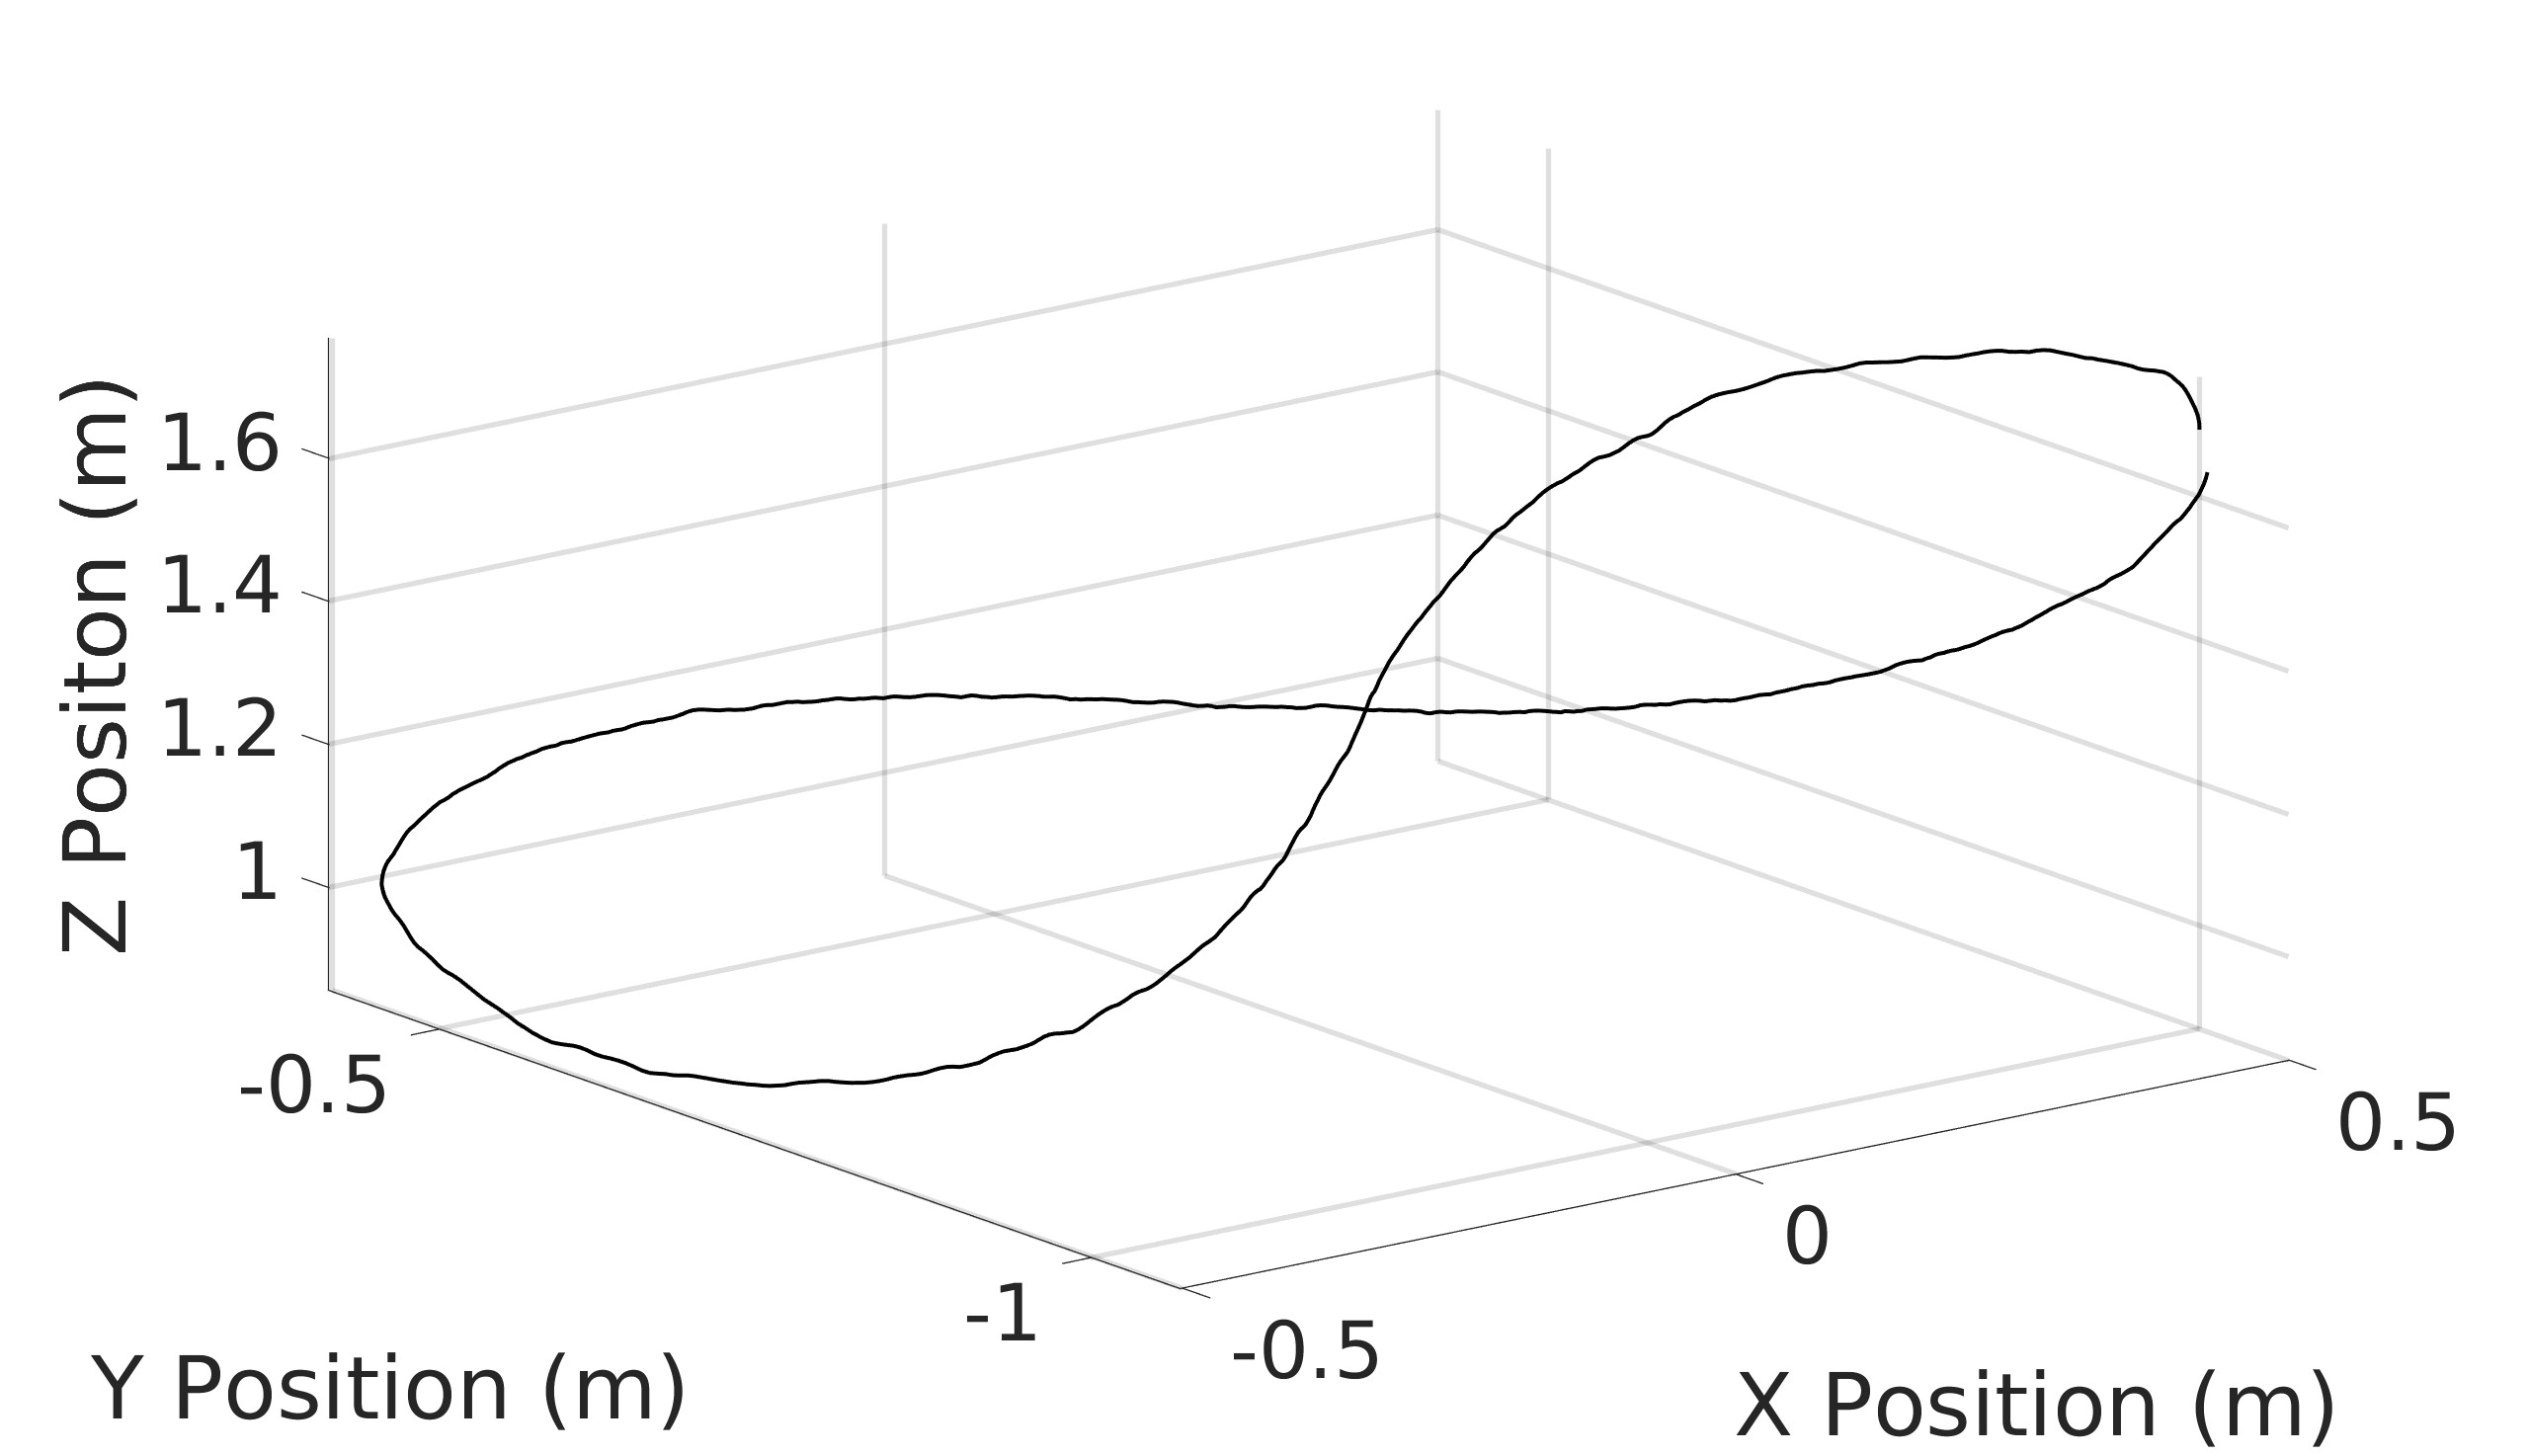
\includegraphics[width=1\textwidth]{plots/traj2.jpg}
            \caption{Infinity Symbol Trajectory Tracking of Stochastic Position Controller}
            \label{traj2}
    \end{figure}\clearpage
    Another trajectory was passed to the agent to ensure that it learned to track any given trajectory. Fig. \ref{traj1} shows a helix trajectory with a radius of 1 meter and the agent climbing 1 meter during the 3 cycles around the helix. The agent was able to successfully track the given trajectoyy. Small oscillations appear in the $z$ direction however, this is due to the acrobatic nature of the CrazyFlie quadcopter making it sensitive to small changes in thrust values causing the oscillations.
    \begin{figure}[H]
            \centering
            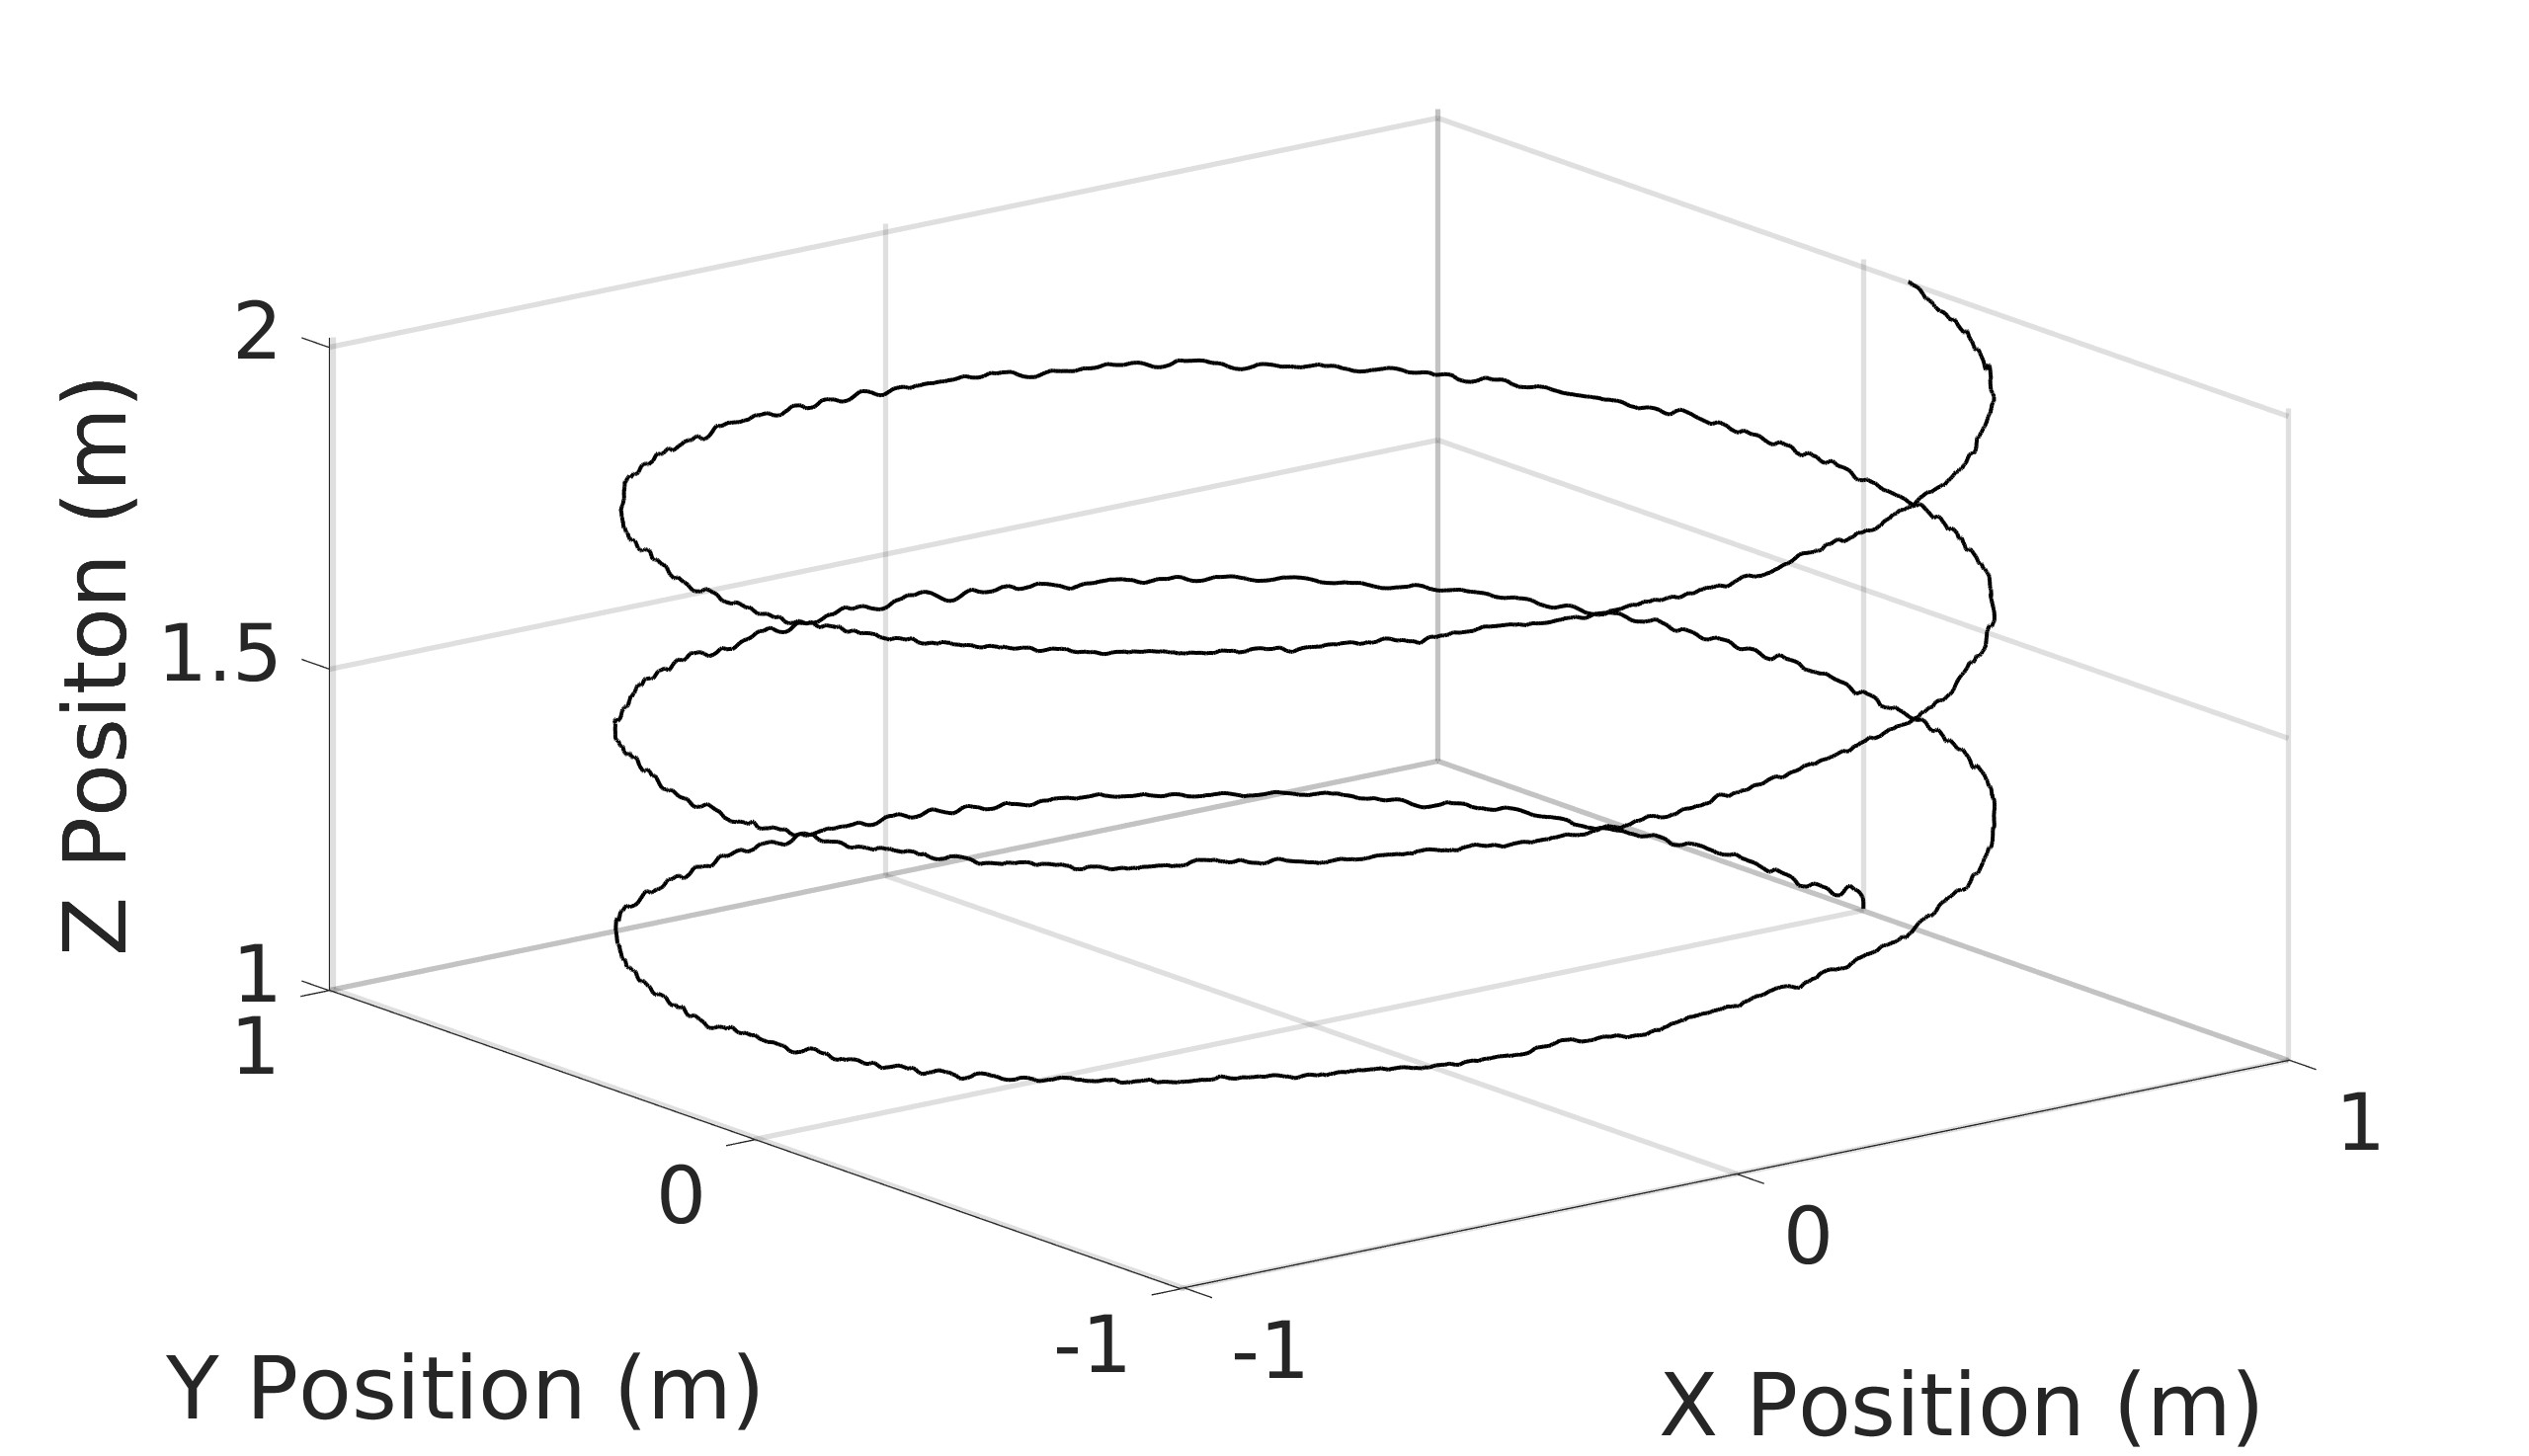
\includegraphics[width=1\textwidth]{plots/traj1.jpg}
            \caption{Helix Trajectory Tracking of Stochastic Position Controller}
            \label{traj1}
    \end{figure}\clearpage
    %#####################################################################
    \section{External Disturbances}
    To test the robustness of the proposed controller, the controller was subjected to external disturbances in the form of wind disturbances. To simulate the wind effect, external noise was added to the Euler rates of the quadcopter. With each time step a random euler rate is assigned to the quadcopter increasing and decreasing randomly with the controller trying to eliminate their effect. Fig. \ref{traj2w} shows that the controller was able to eliminate most of the disturbances and maintain a smooth trajectory. 
    \begin{figure}[H]
            \centering
            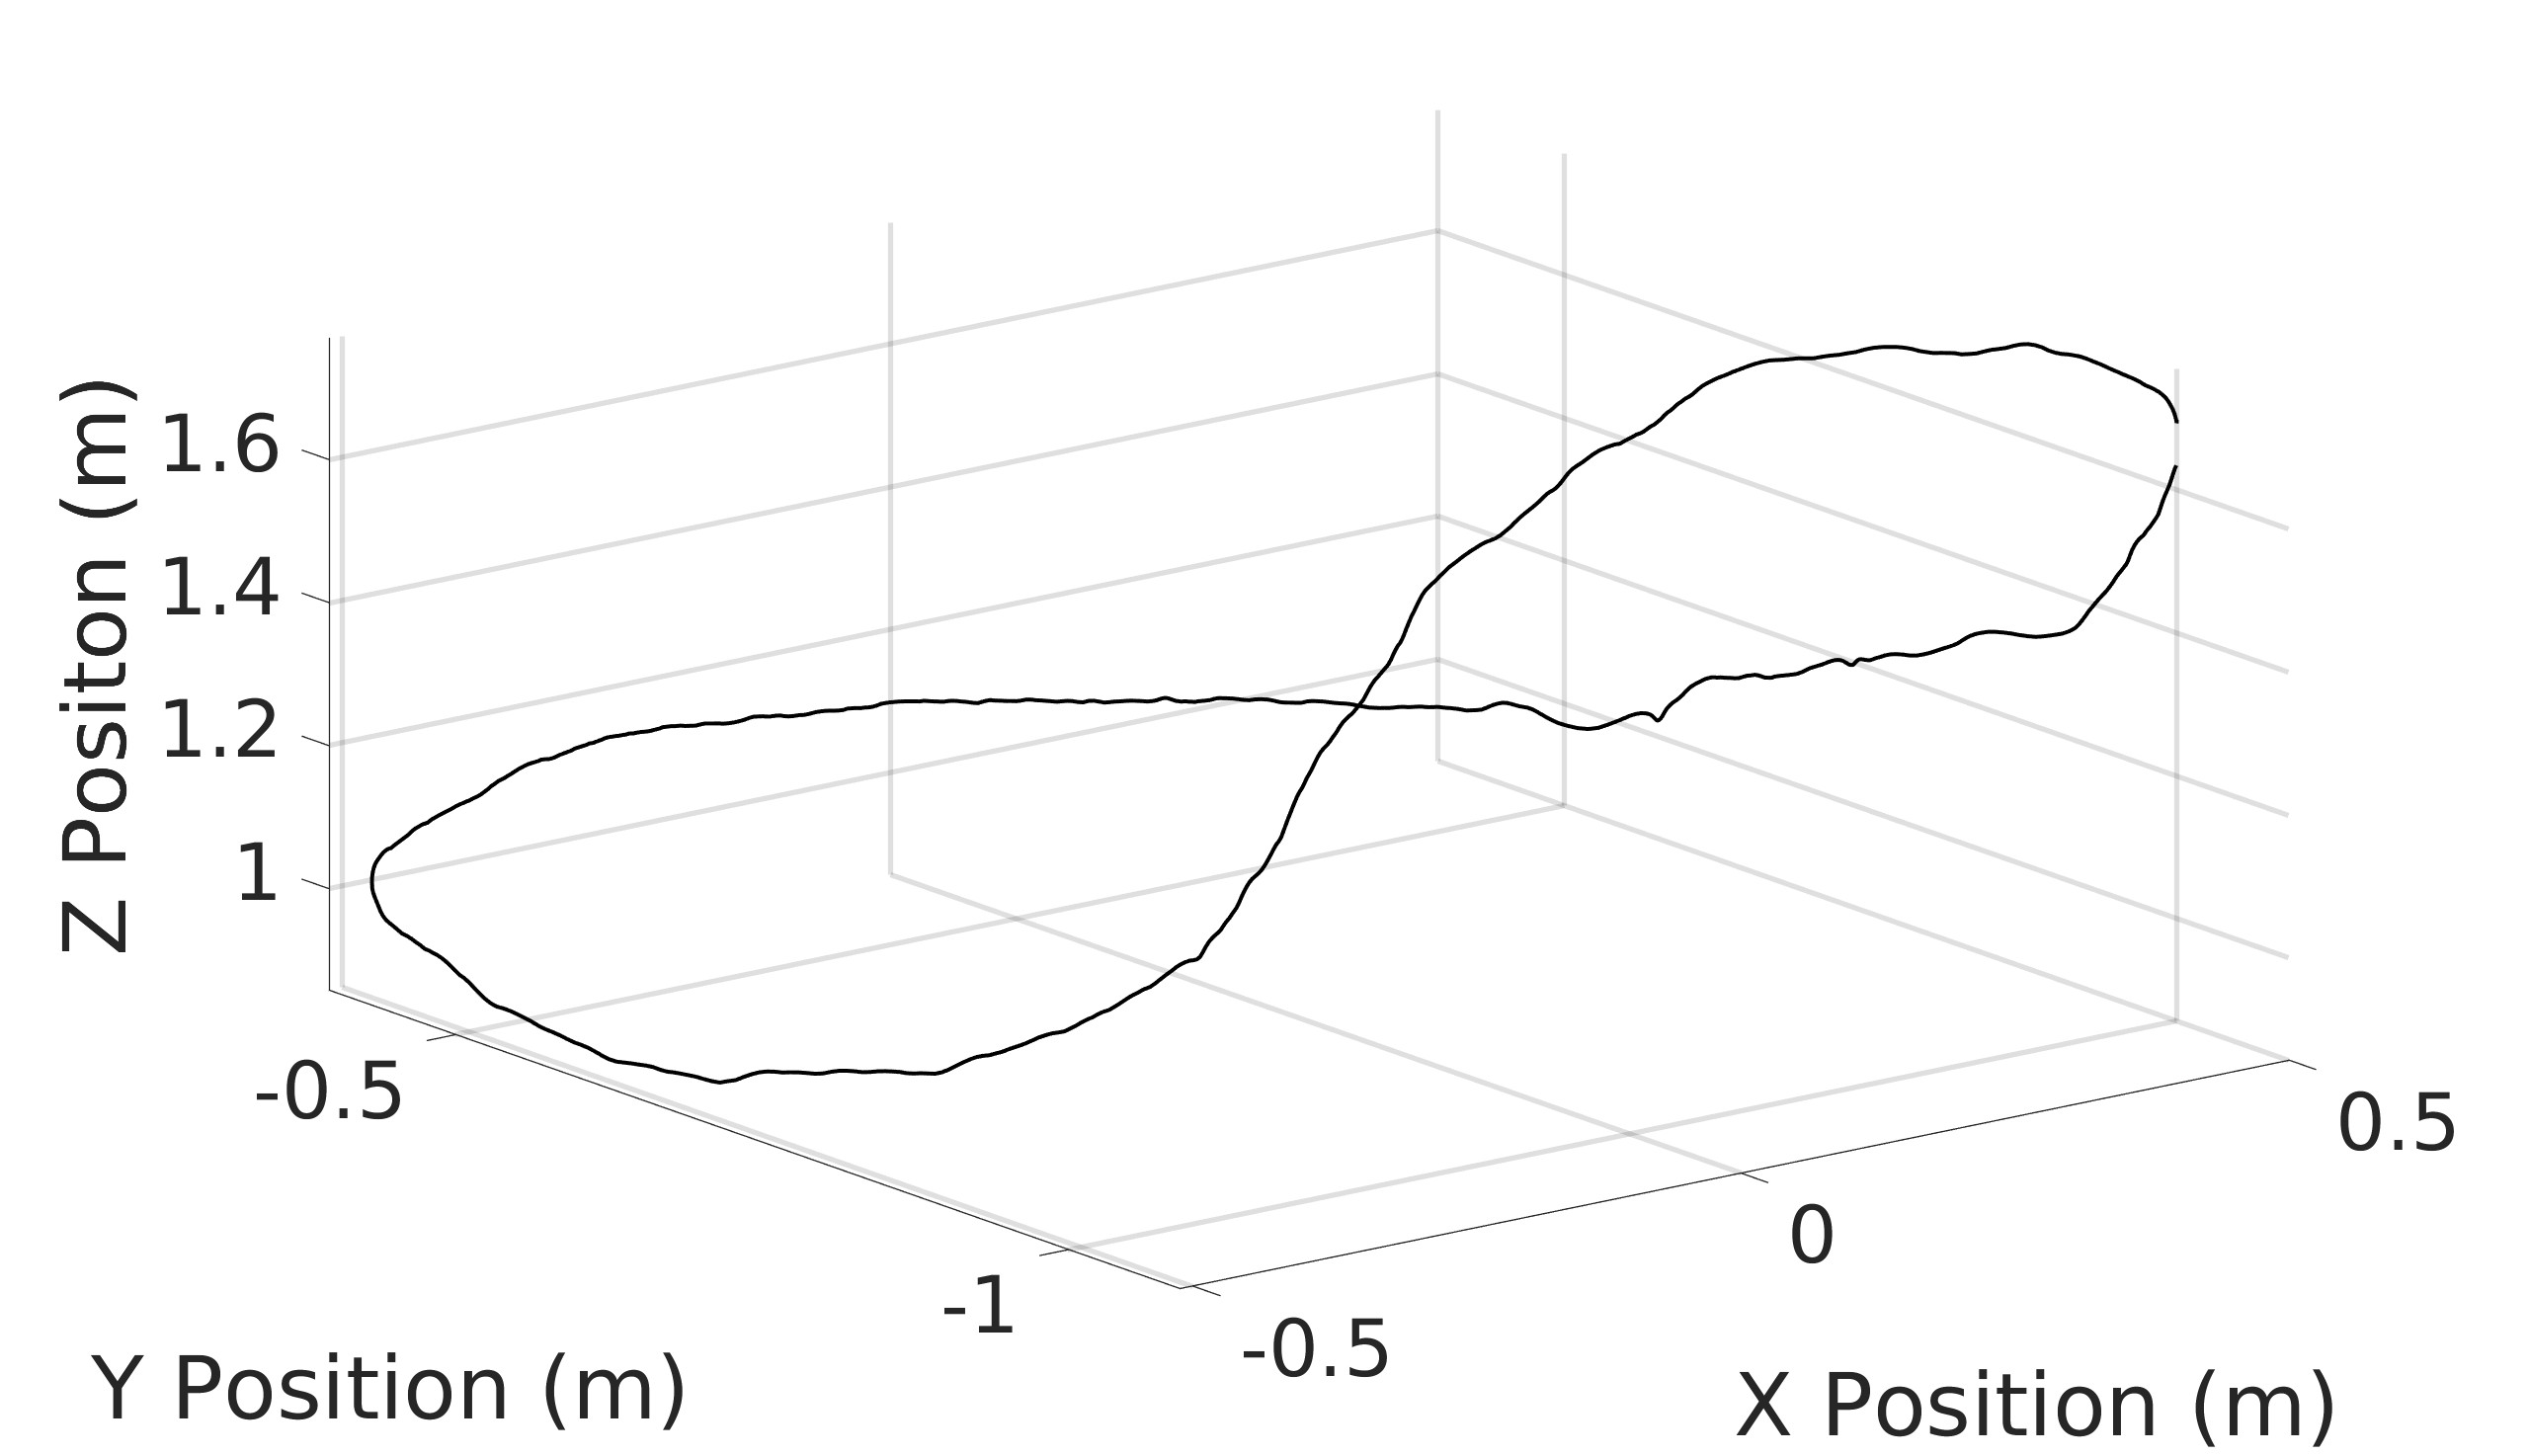
\includegraphics[width=1\textwidth]{plots/traj2W.jpg}
            \caption{Infinity Symbol Trajectory Tracking of Stochastic Position Controller with Wind Disturbance}
            \label{traj2w}
    \end{figure}\clearpage
    Fig. \ref{traj1w} shows the controller maintaining the helix trajectory while trying to minimize the disturbances and staying on track. Higher oscillations are present in this trajectory compared to the previous one.
    \begin{figure}[H]
            \centering
            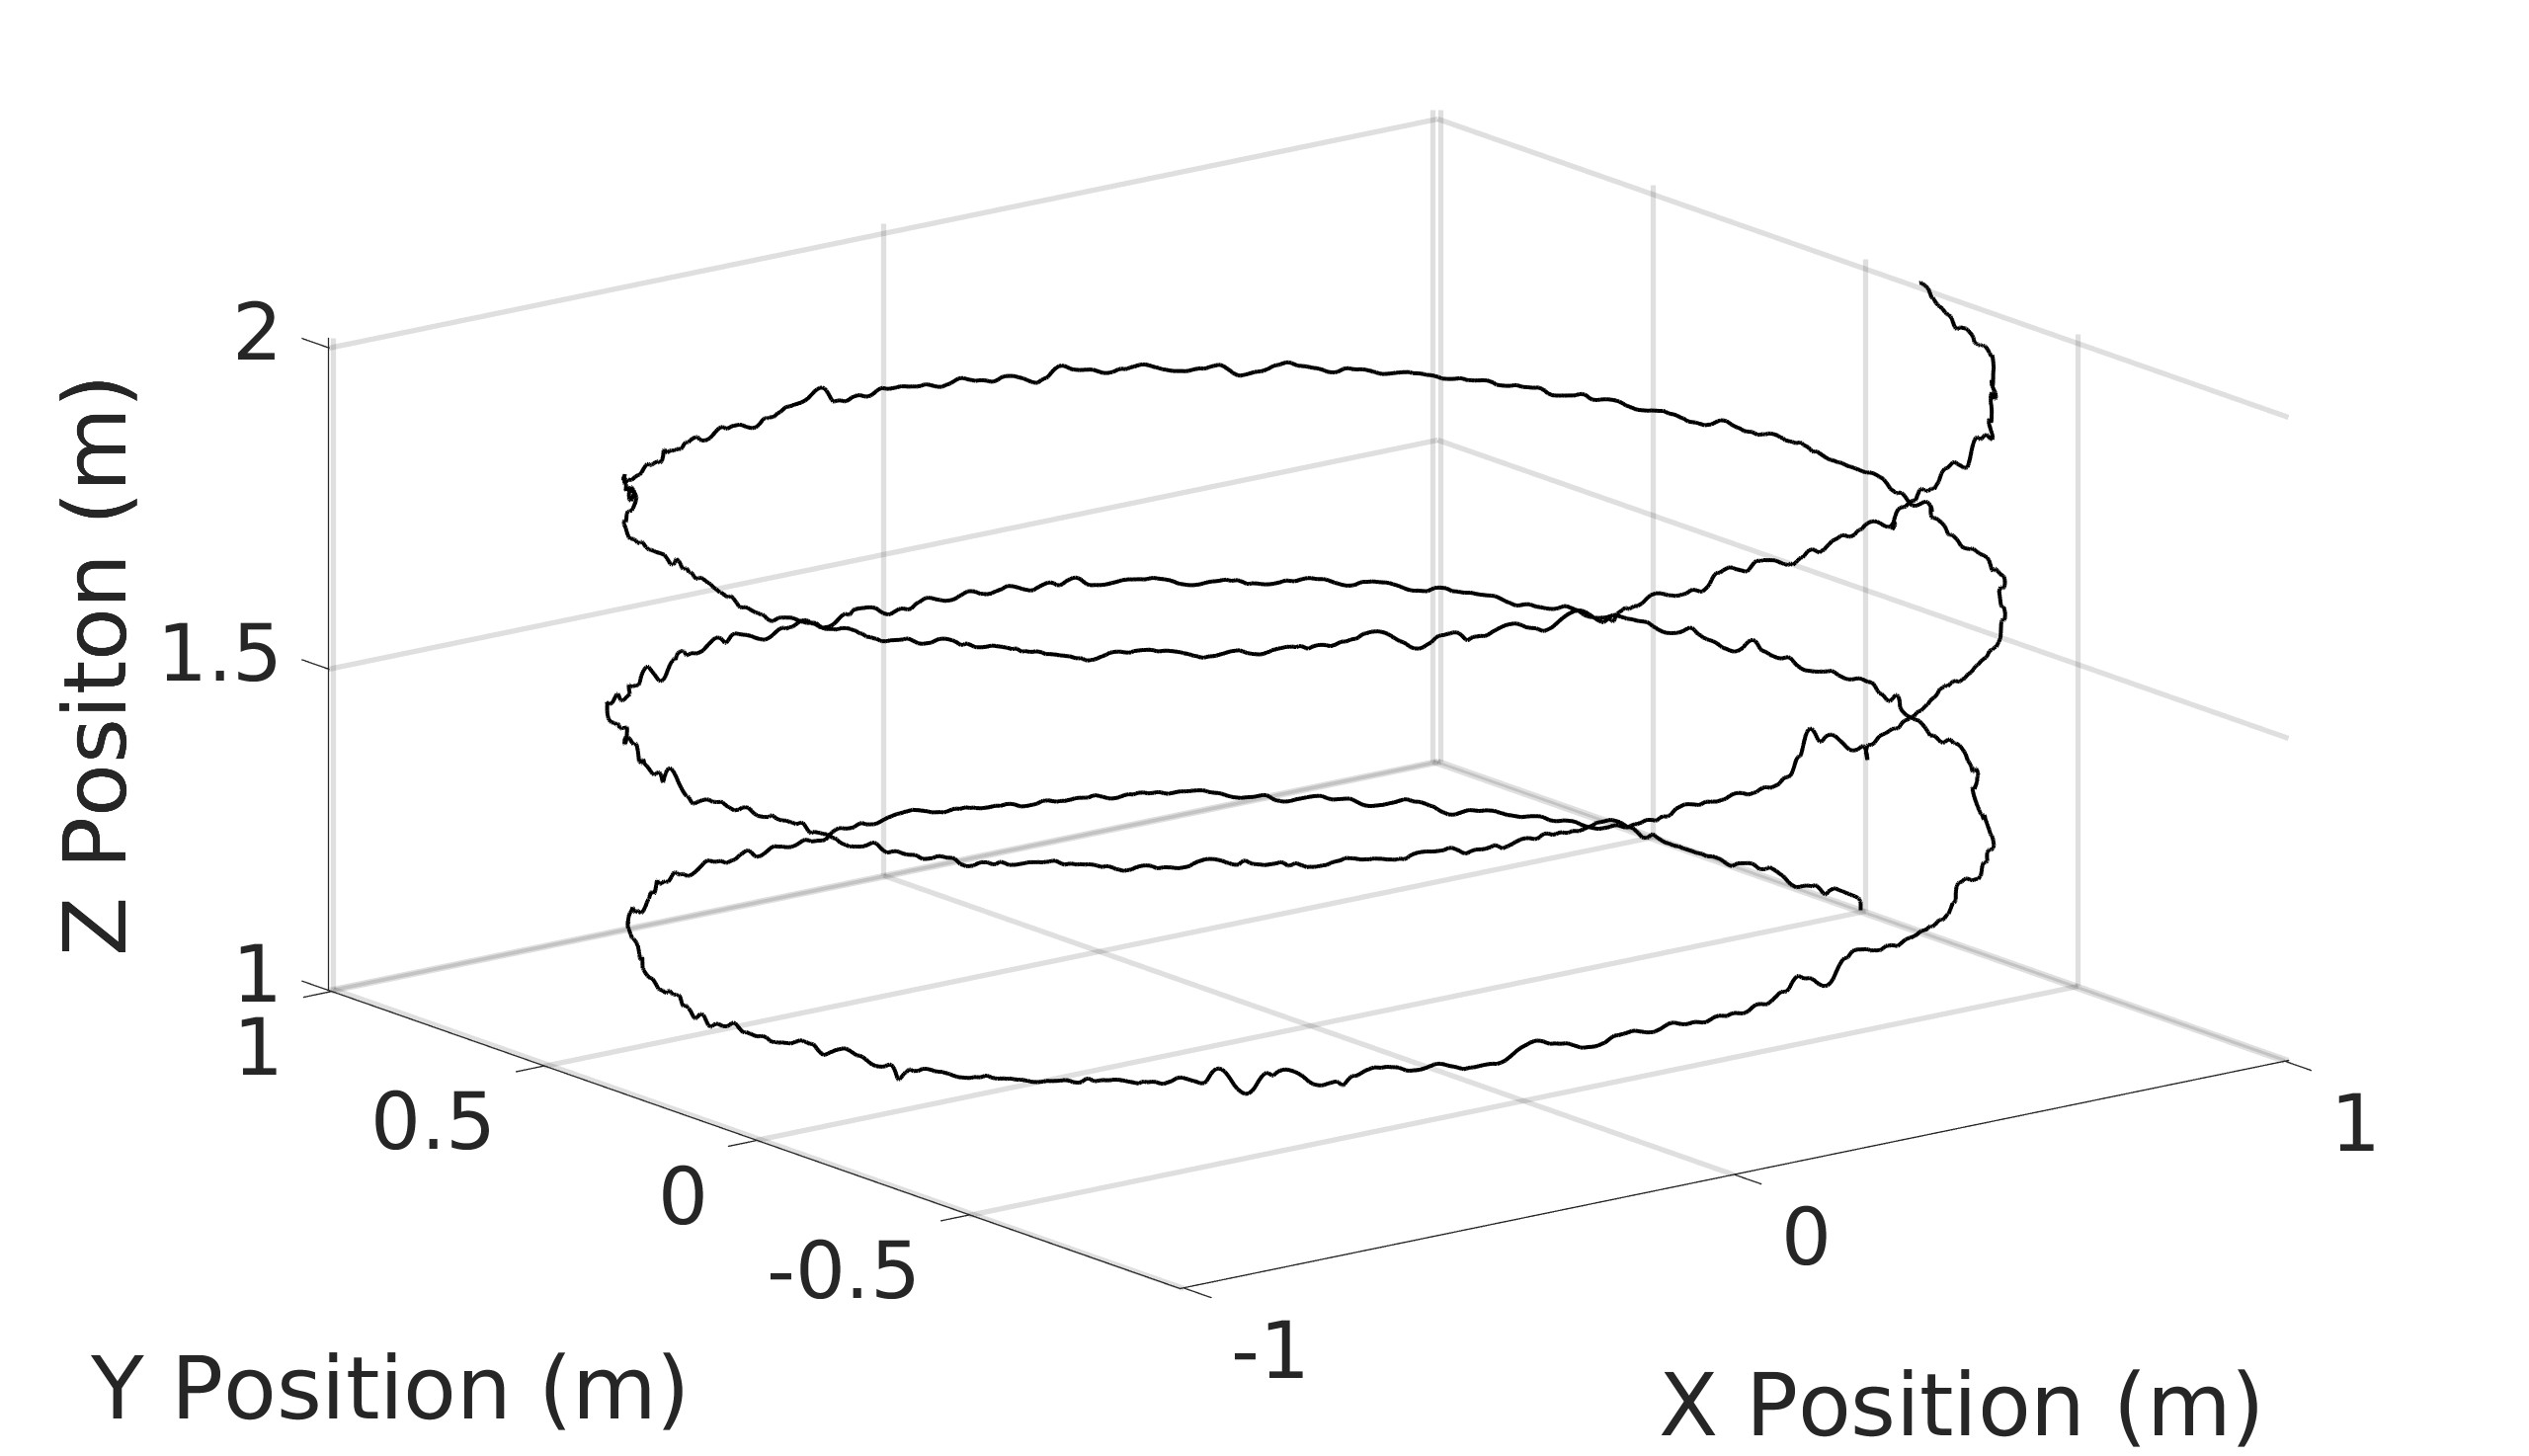
\includegraphics[width=1\textwidth]{plots/traj1W.jpg}
            \caption{Helix Trajectory Tracking of Stochastic Position Controller with Wind Disturbance}
            \label{traj1w}
    \end{figure}
    The results obtained show the adaptability of the controller with unseen environment conditions such as wind disturbances. The controller effectively minimizes their effect and keeps track of the trajectory.\clearpage
    %####################################################################
    \section{Different Dynamics}
    A main issue with the proposed low-level controllers that maps environment states to motor commands in the literature is their lack of compatibility. This is due to these controllers controlling the motor RPMs directly. As the agent is transferred from one quadcopter to another, the agent needs to be retrained to adapt to the new quadcopter dynamics as not all quadcopters have the same thrust-to-weight coefficients, weight, and various other dynamics of the quadcopters. Without further training, the agent fails to pilot the quadcopter as shown in the next results.\\

    The proposed position controller on the other hand calculates only the desired thrust and orientation and sends these data to a PID attitude controller. The attitude controller takes care of the different dynamics of the quadcopter. This helps extend the compatibility of the agent with various quadcopters.\\

    Gym-pybullet-drones offers 2 different CrazyFlie quadcopters with two different orientations, a QuadX and a Quad+ copter shown in Fig. \ref{quads}.
    \begin{figure}[H]
            \centering
            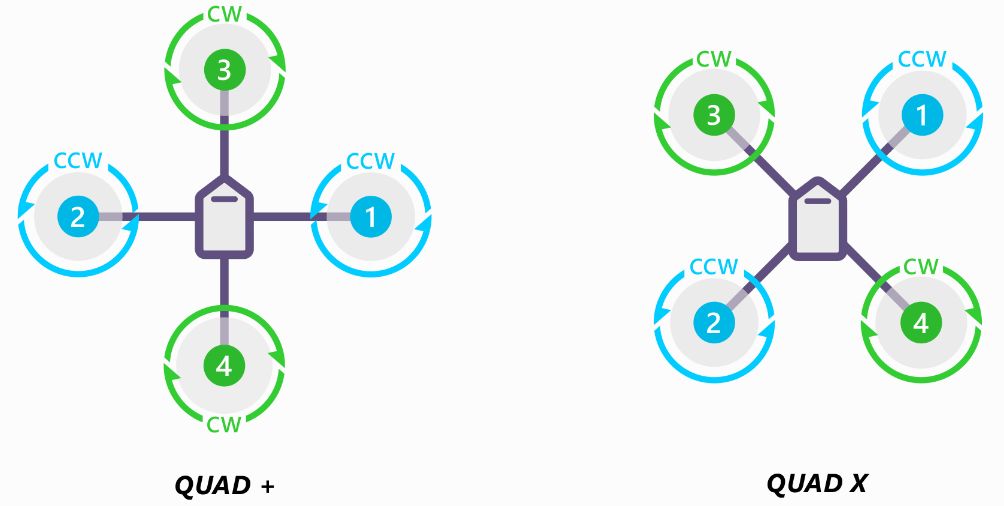
\includegraphics[width=0.8\linewidth]{Images/Quad.png}
            \caption{QuadX and Quad+ Quadcopter Configurations \cite{arducopter}}
            \label{quads}
    \end{figure}\clearpage
    The stochastic path-following controller, and the position controller are both trained using the QuadX configuration. The controllers were tested on a Quad+ configuration without any prior training. Fig. \ref{psac} shows that the path-following controller failed to navigate the quadcopter and crashed almost instantly.
    \begin{figure}[H]
            \centering
            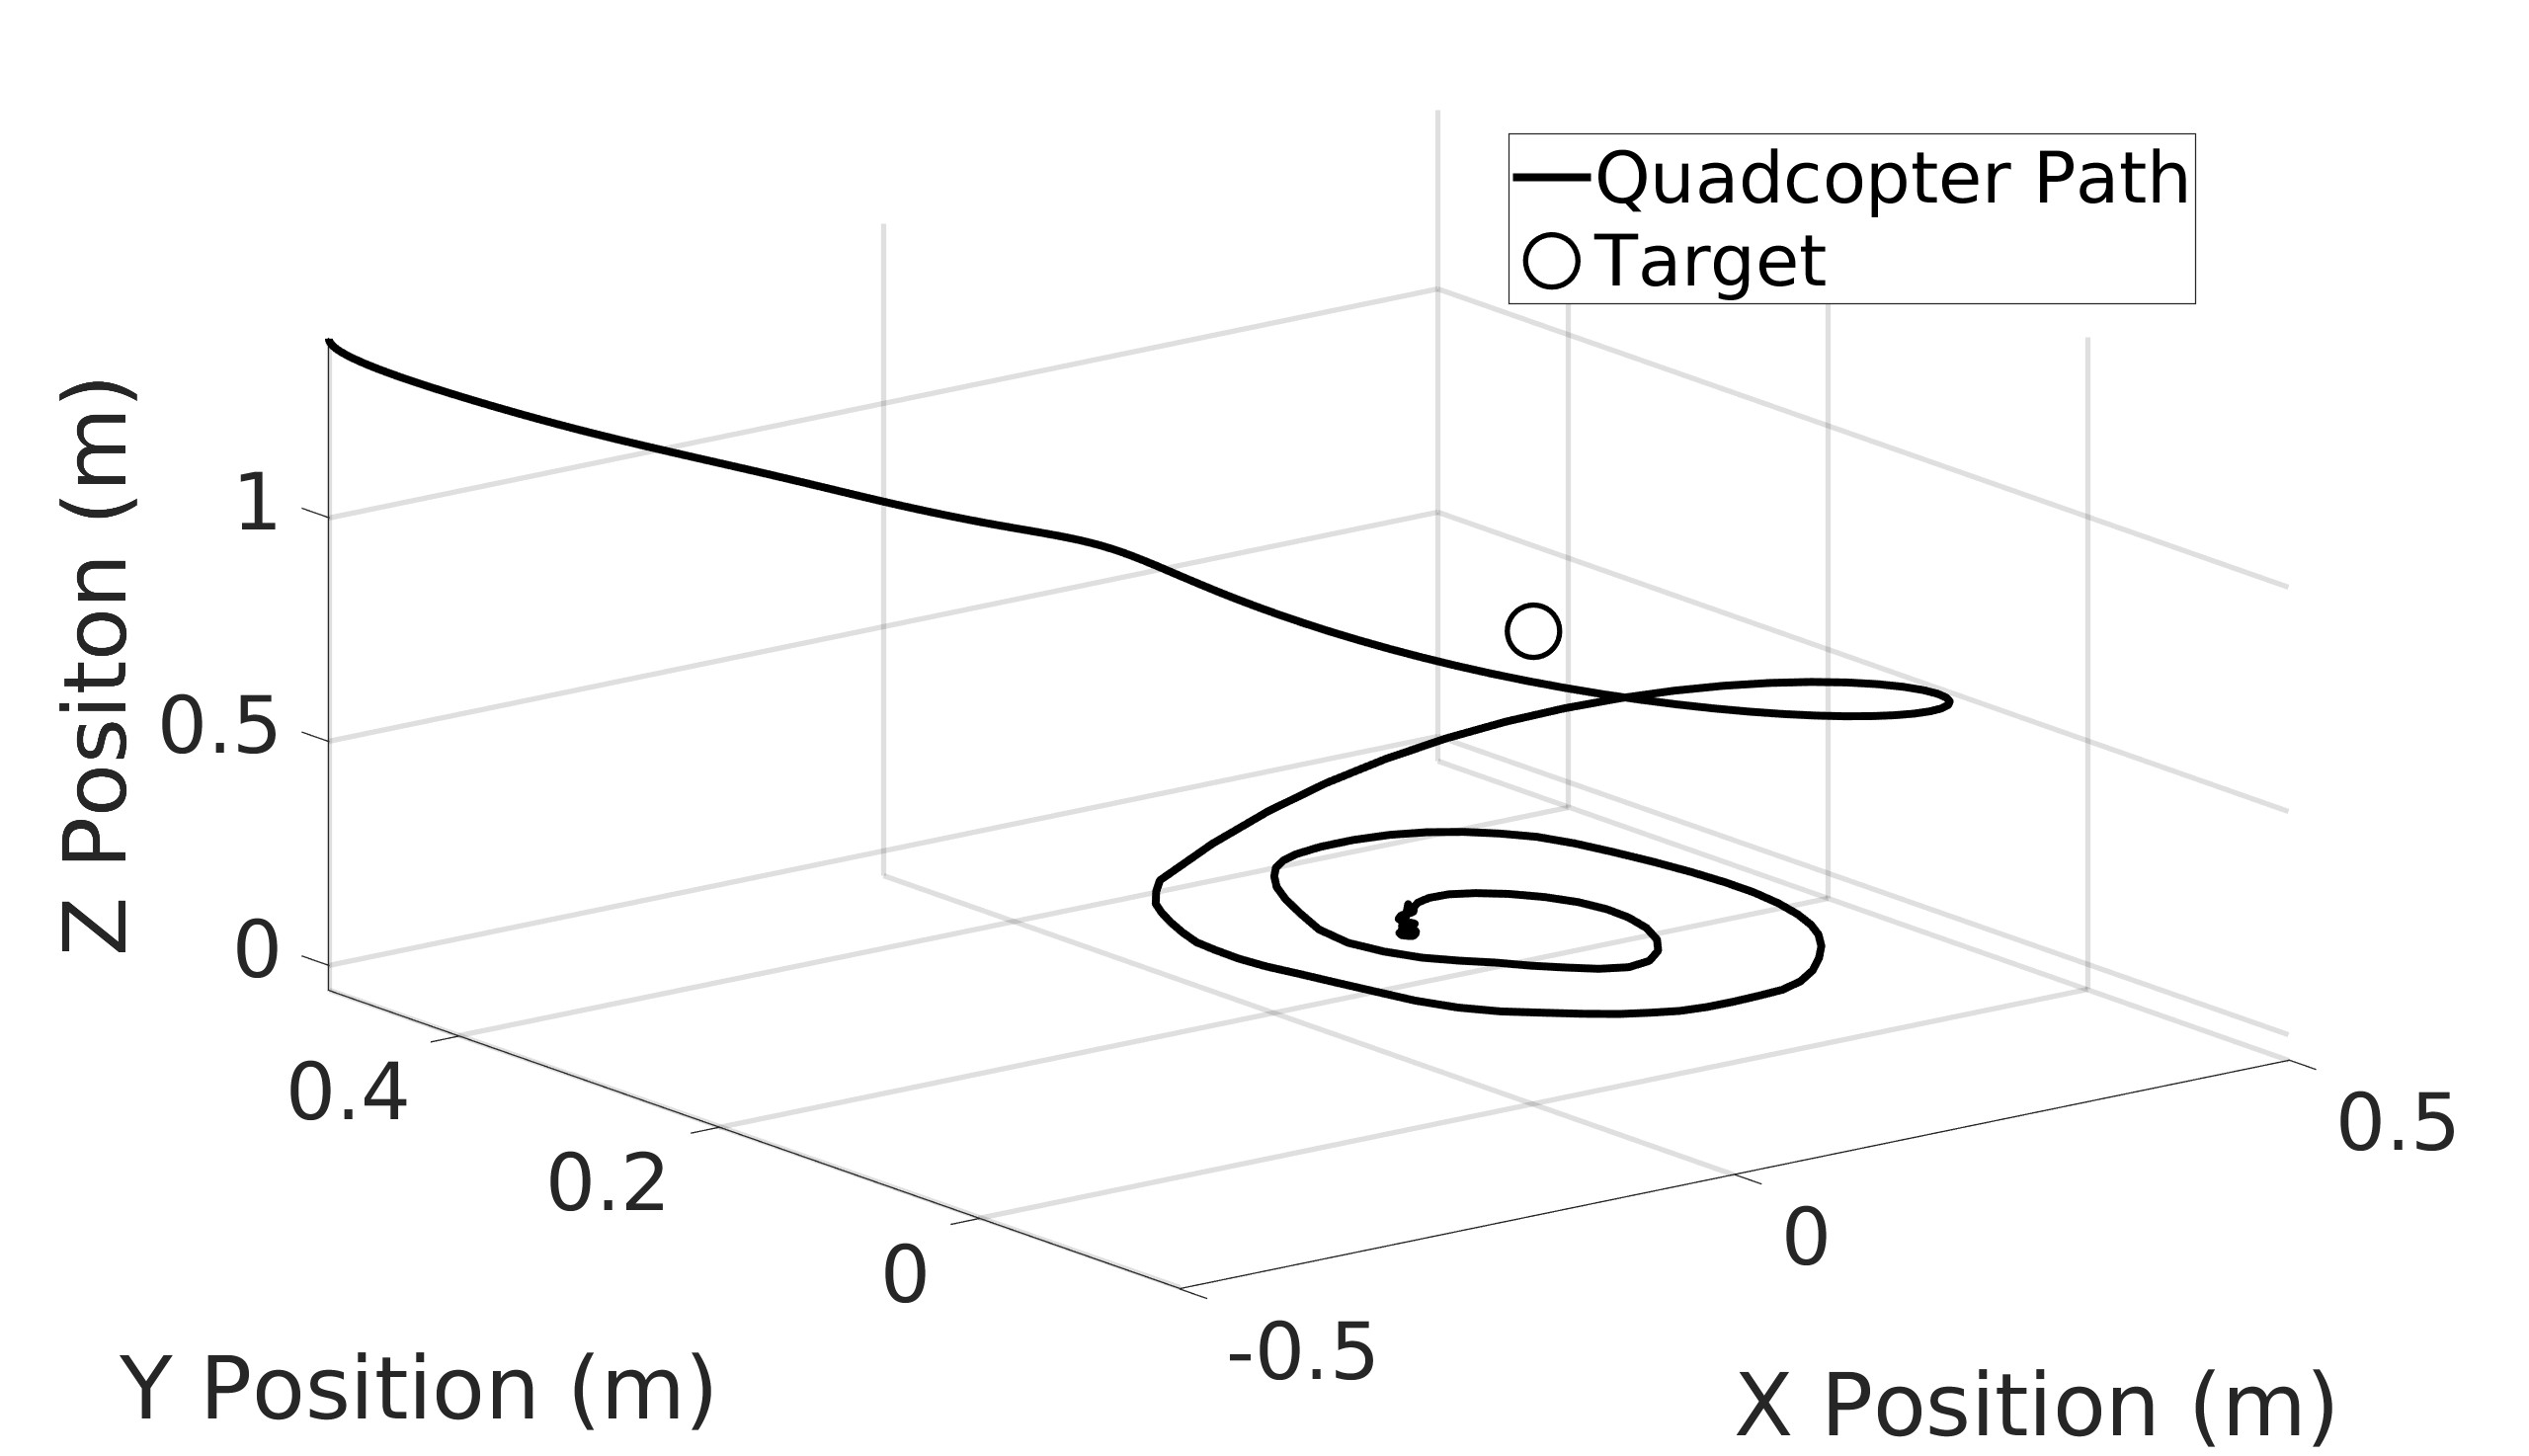
\includegraphics[width=0.85\textwidth]{plots/p_crash.jpg}
            \caption{Quad+ Configuration Response of Path-following Stochastic Controller}
            \label{psac}
    \end{figure}
    Fig. \ref{stabp} shows the response of the position controller. The results are almost identical to those of the QuadX configuration. This is due to the PID controller taking care of the different dynamics of each quadcopter.
    \begin{figure}[H]
            \centering
            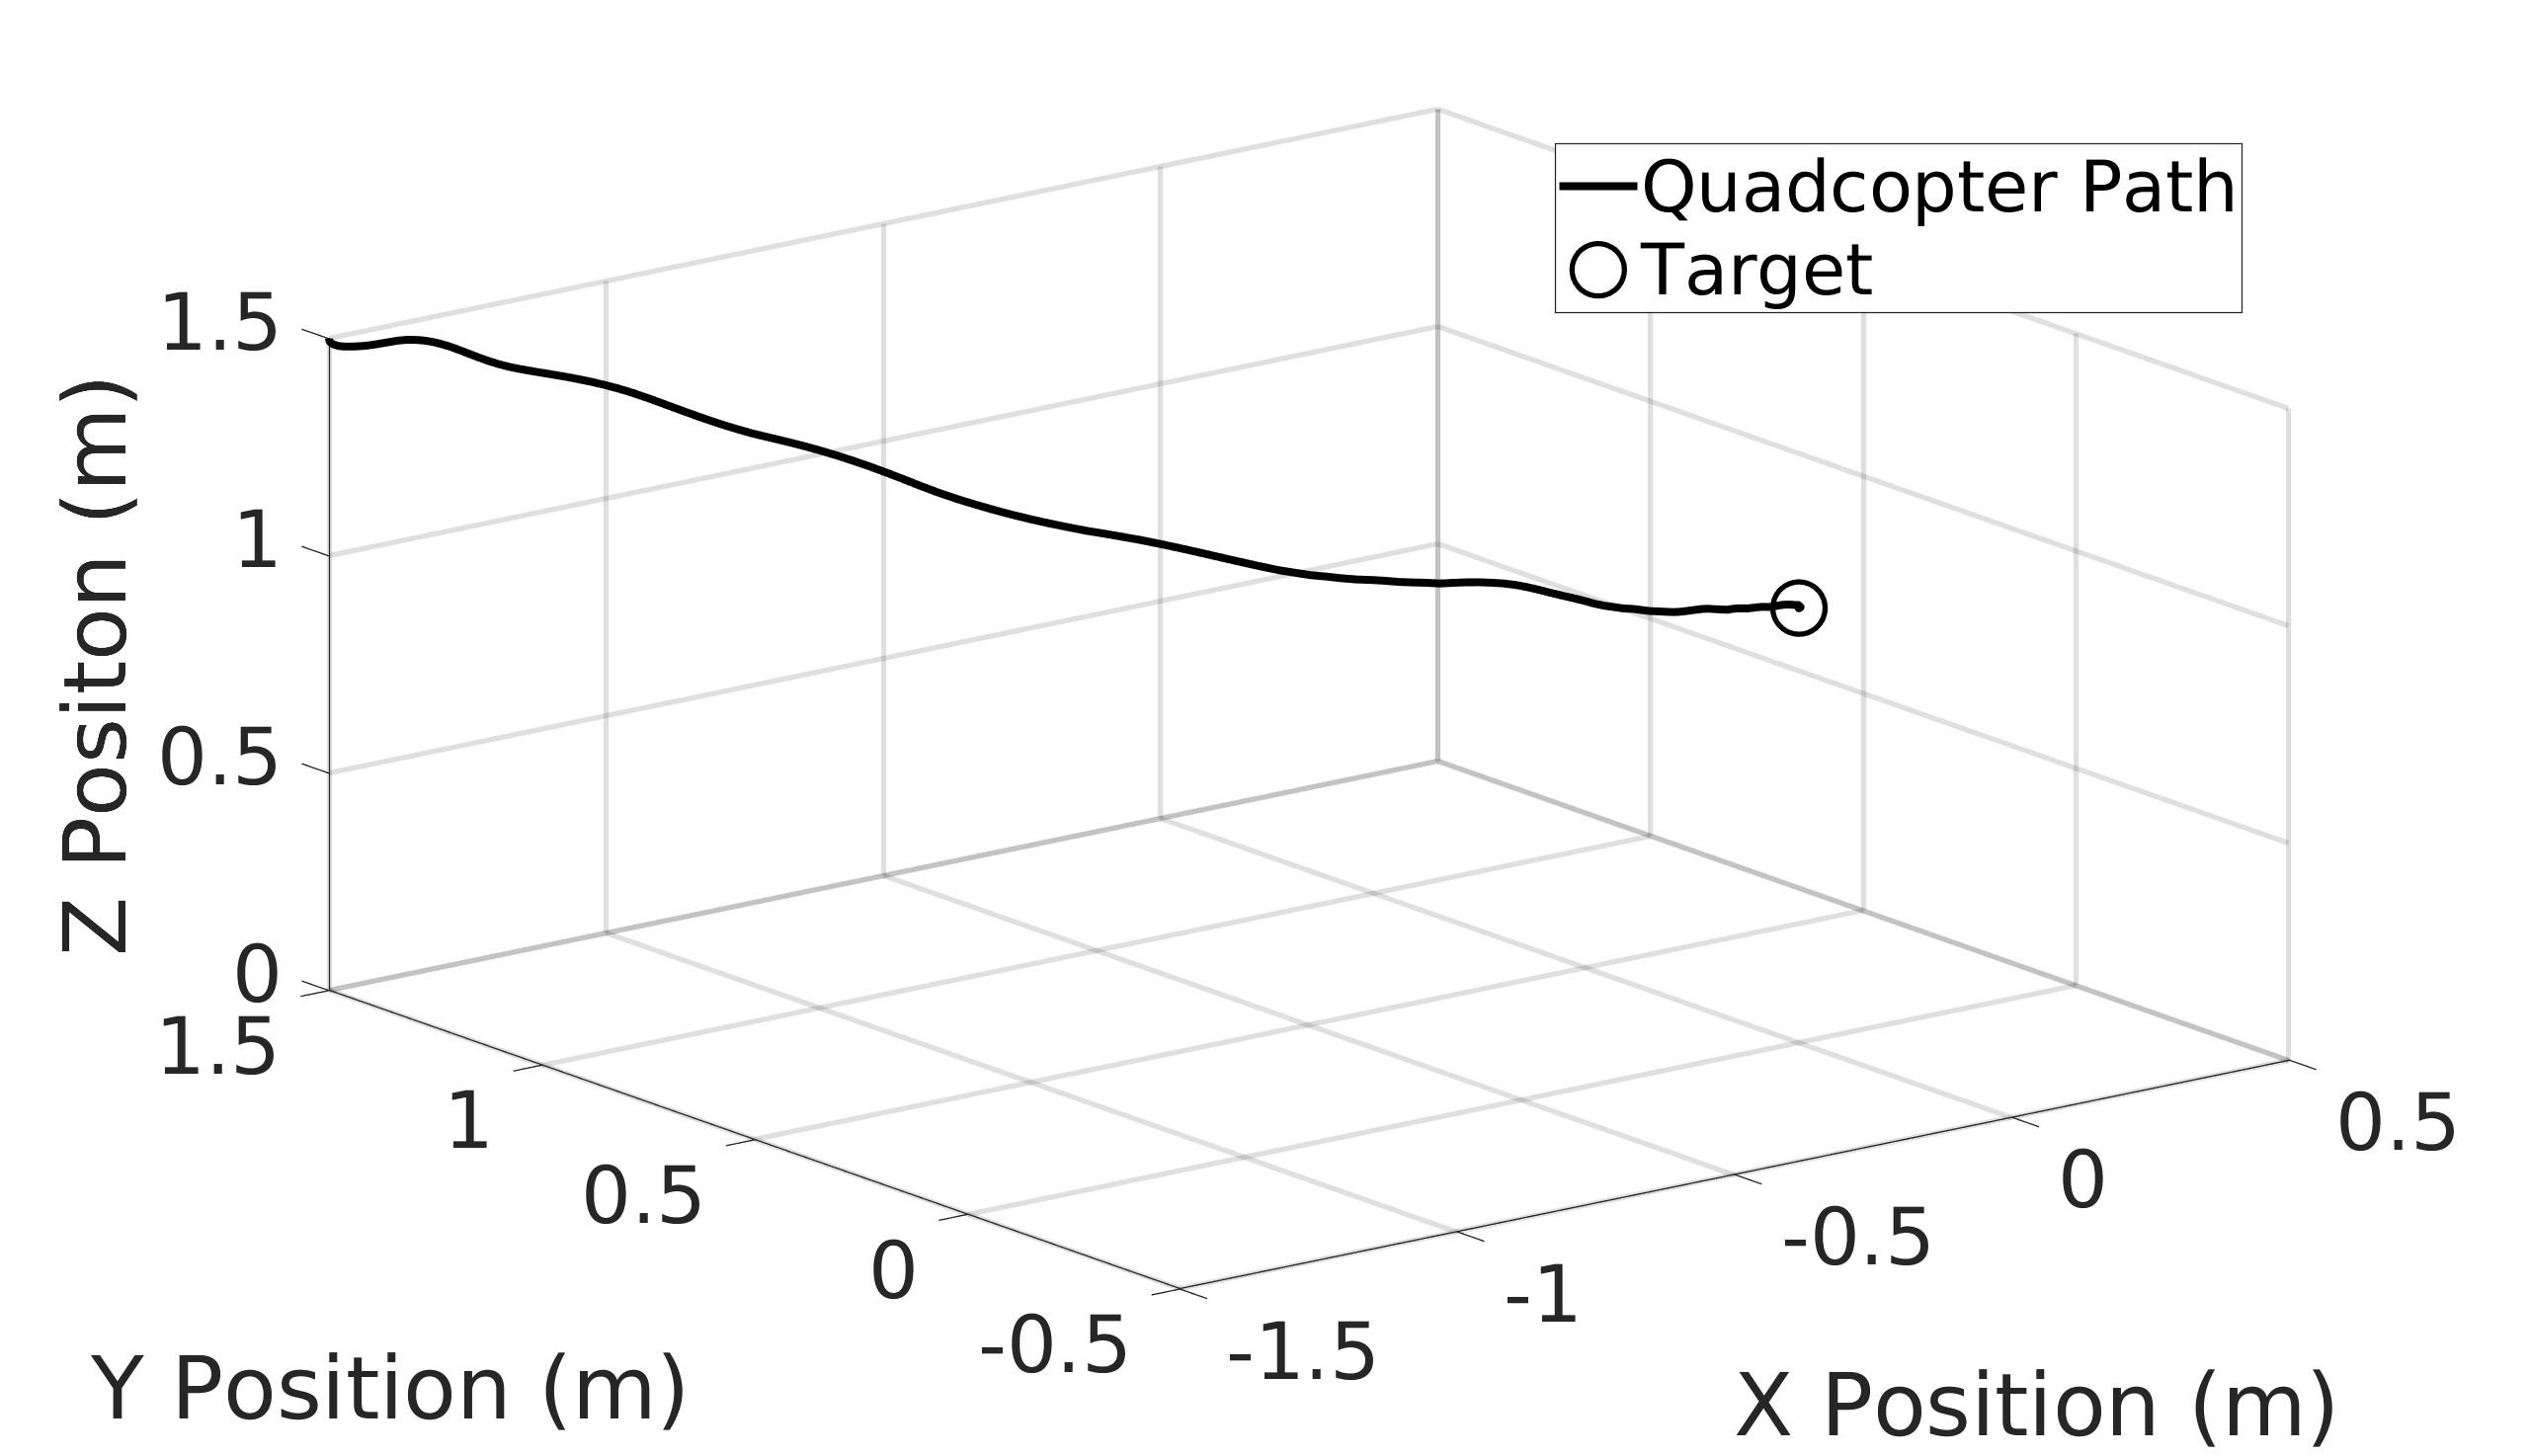
\includegraphics[width=0.85\textwidth]{plots/p_sac.jpg}
            \caption{Quad+ Configuration Response of Stochastic Position Controller}
            \label{stabp}
    \end{figure}
    The stochastic position controller was tested with a trajectory and the quadcopter gave almost identical results to that of the QuadX configuration. Fig. \ref{traj2p} shows the smooth tracking of the given trajectory.
    \begin{figure}[H]
            \centering
            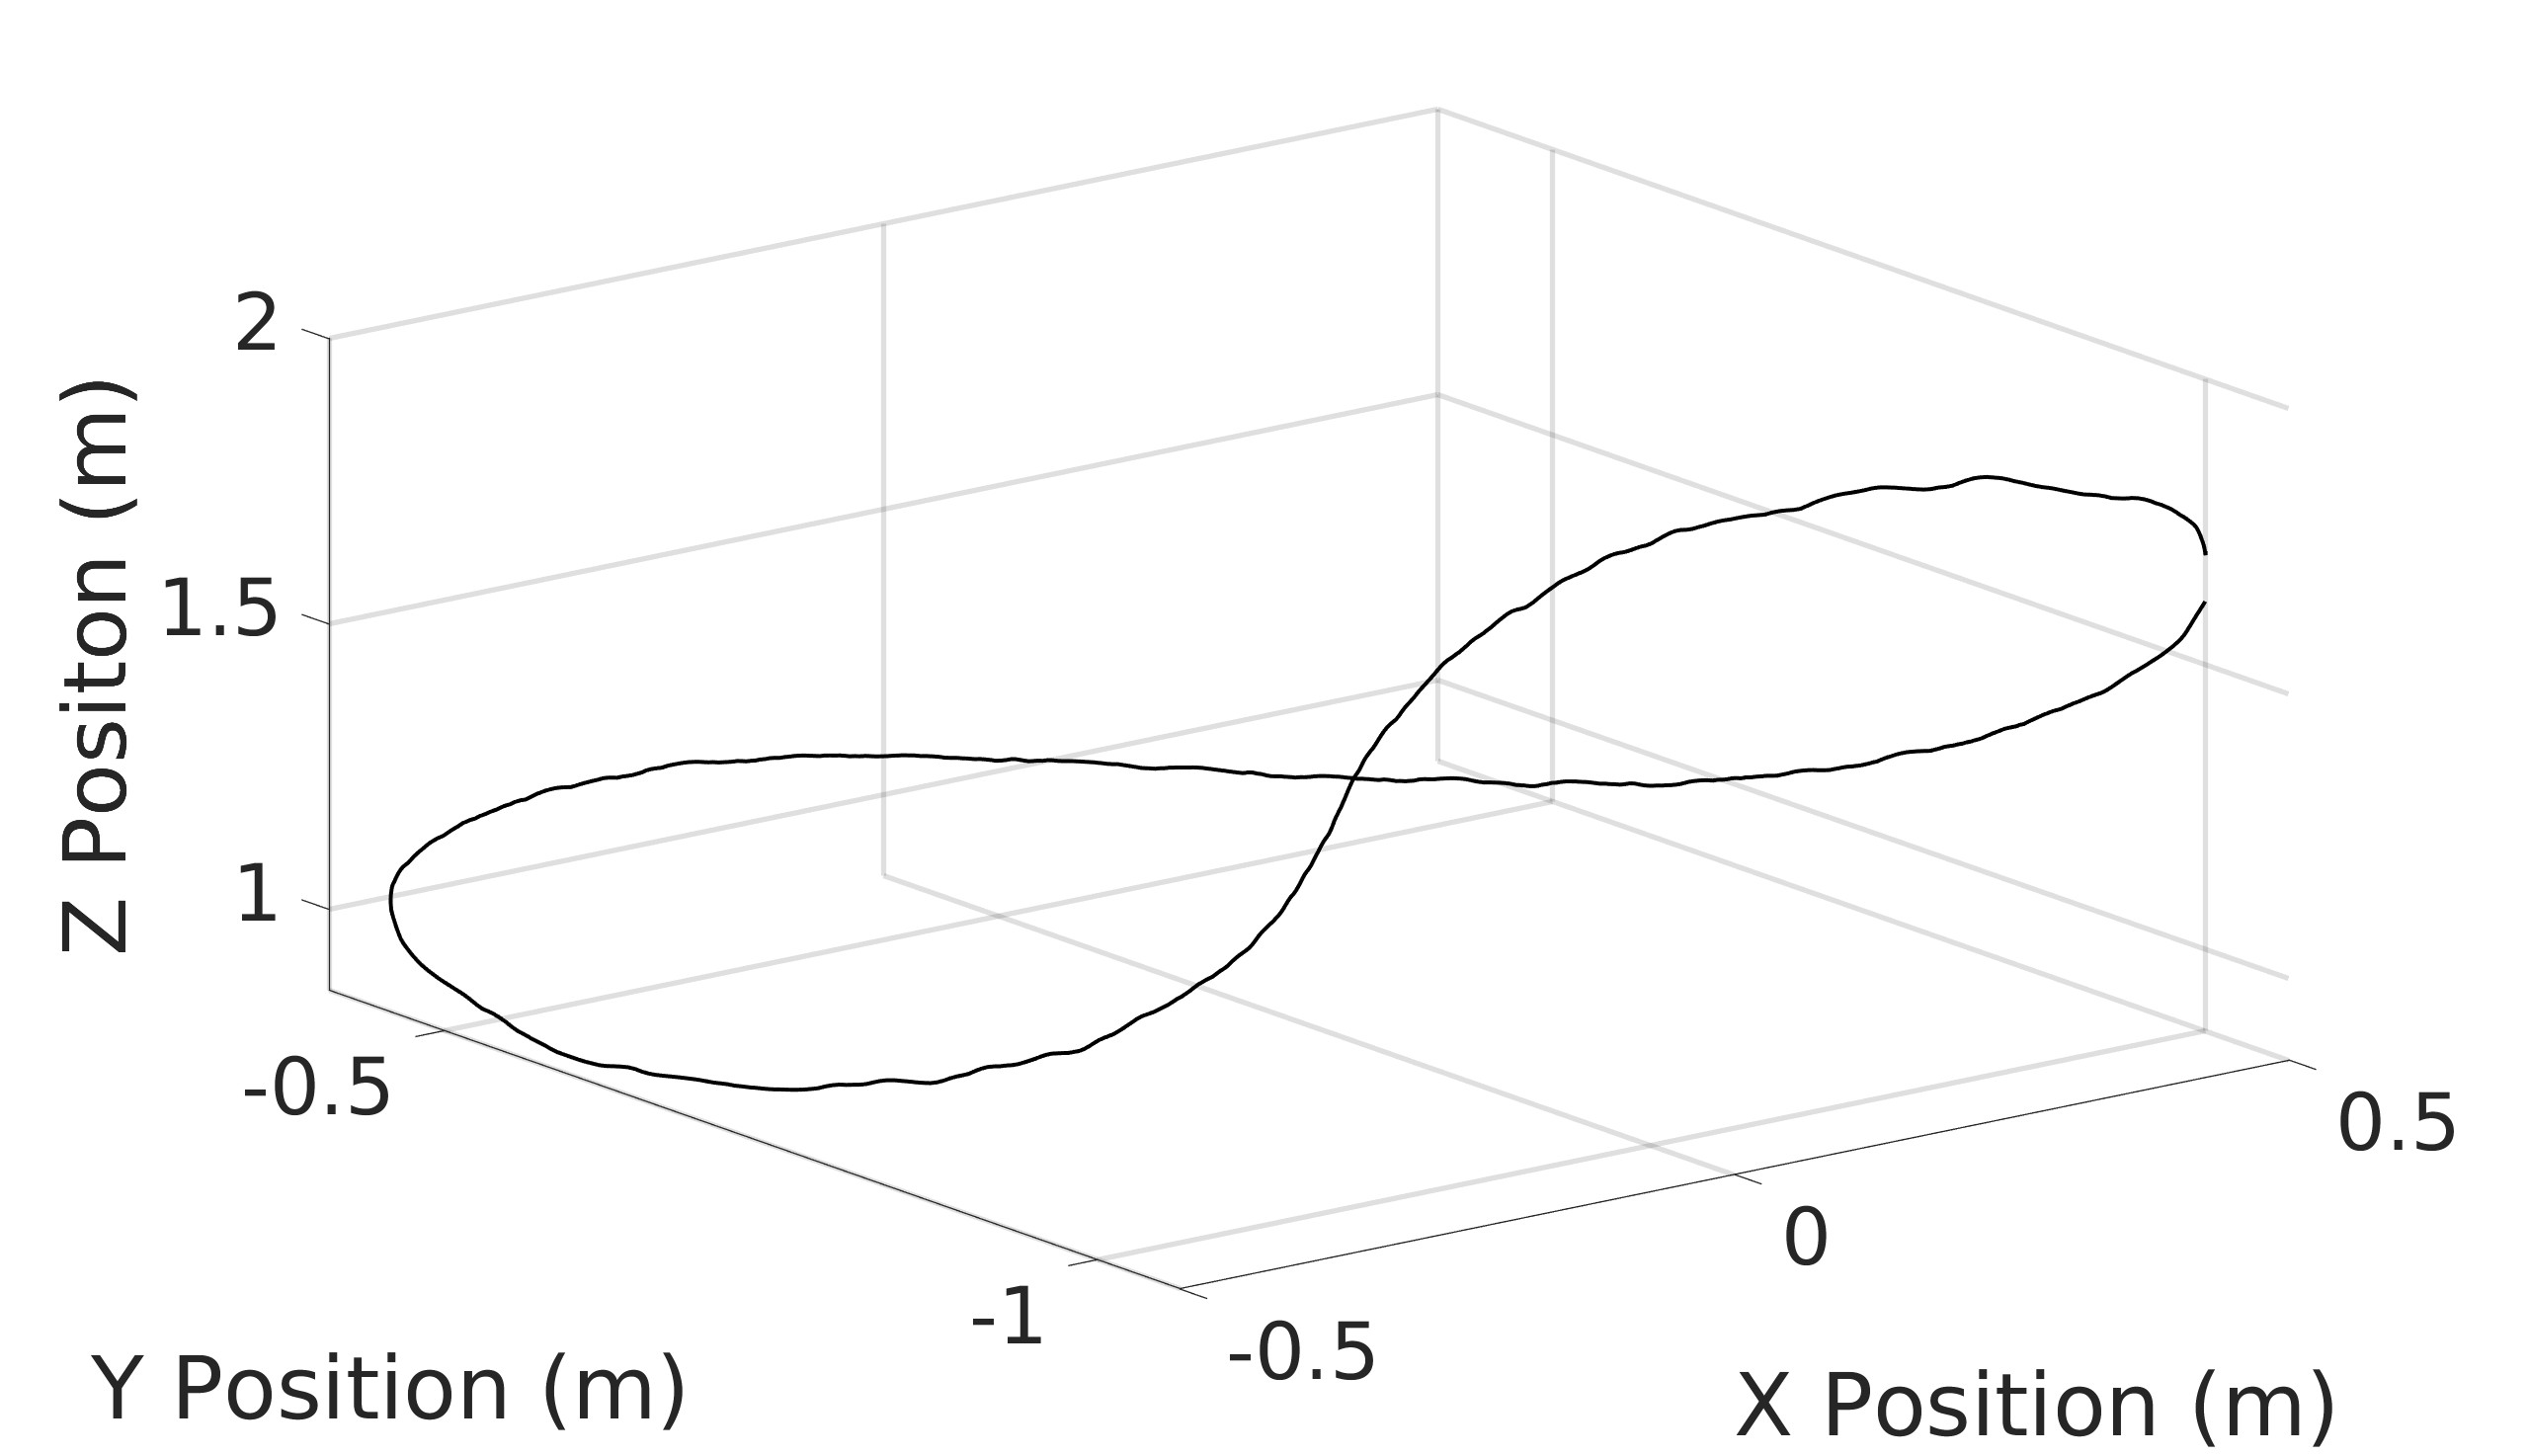
\includegraphics[width=1\textwidth]{plots/traj2P.jpg}
            \caption{Infinity Symbol Trajectory of Stochastic Position Controller with Quad+ Configuration}
            \label{traj2p}
    \end{figure}
    The results obtained show the compatibility of the controller with different kinds of quadcopters in contrast to the low-level controllers that control the motor commands directly. As the results showed, even the slightest change in the quadcopter dynamics, such as changing motor configurations, affects the low-level controller negatively. On the other hand, the position controller can be integrated with any quadcopter given the suitable attitude controller.
    %#####################################################################